%                               dpic-doc.tex
\documentclass[11pt]{article}
\usepackage{verbatim,url}
\usepackage{amssymb}
\usepackage{graphicx}
\usepackage{multicol}
\usepackage{xspace}
\usepackage{wrapfig}
\usepackage{troffman}
\usepackage{tikz}
\usepackage{boxdims}
%                               Fix the table of contents:
\usepackage{tocloft}
%                               For links
\usepackage{bookmark}
\usepackage{pdfcomment}
%                               Fonts
\usepackage[T1]{fontenc}
\usepackage{lmodern}
%                               Adjust the page size
\addtolength{\textwidth}{3cm}
\addtolength{\hoffset}{-1.5cm}
\addtolength{\voffset}{-1.5cm}
\addtolength{\headsep}{-0.5cm}
\addtolength{\textheight}{4cm}
\setcounter{topnumber}{3}
%                               Minimum hyphenation length
\lefthyphenmin=3
\righthyphenmin=3
%                               Left-justified captions
\makeatletter
\long\def\@makecaption#1#2{%
  \vskip\abovecaptionskip
  \sbox\@tempboxa{#1: #2}%
  \ifdim \wd\@tempboxa >\hsize
    #1: #2\par
  \else
    \global \@minipagefalse
    \hb@xt@\hsize{\box\@tempboxa\hfil}%
  \fi
  \vskip\belowcaptionskip}

%\def\@date{February 01, 2015}
\makeatother
%                               Customizations
\newcommand{\bq}{}
\newcommand{\pic}{{\bq pic}\xspace}
\newcommand{\dvips}{{\bq dvips}\xspace}
\newcommand{\Pic}{{\bq Pic}\xspace}
\newcommand{\gpic}{{\bq gpic}\xspace}
\newcommand{\Gpic}{{\bq Gpic}\xspace}
\newcommand{\Dpic}{{\bq Dpic}\xspace}
\newcommand{\tpic}{{\bq tpic}\xspace}
%\renewcommand{\LaTeX}{{LaTeX}\xspace}
\newcommand{\mfpic}{{\bq mfpic}\xspace}
\newcommand{\groff}{{\bq groff}\xspace}
\newcommand{\xfig}{{\bq xfig}\xspace}
\newcommand{\PSTricks}{{\bq PSTricks}\xspace}
\newcommand{\MetaPost}{{\bq MetaPost}\xspace}
\newcommand{\Postscript}{{\bq Postscript}\xspace}
\newcommand{\dpic}{{\bq dpic}\xspace}
\newcommand{\Mfour}{{\bq m4}\xspace}
\newcommand{\TPGF}{{\bq Ti{\it k}z~PGF}\xspace}
%
\setlength{\parindent}{0pt}
\addtolength{\parskip}{1ex}
\newcommand{\ntt}[1]{\\\hbox{}\quad{\tt #1}}
\newcommand{\VL}{\hbox{$|$}}
\newcommand{\tRA}{{\tt\char62}}
\newcommand{\tBS}{{\tt\char92}}
\newcommand{\tLB}{{\tt\char123}}
\newcommand{\tRB}{{\tt\char125}}
%
\newcommand{\SR}[1]{\hyperref[#1]{Section~\ref*{#1}}}
\newcommand{\PR}[1]{\hyperref[#1]{page~\pageref*{#1}}}
\newcommand{\FR}[1]{\hyperref[#1]{Figure~\ref*{#1}}}
%
\hypersetup{
 pdflang=English,
 unicode=true,
 colorlinks=true,
 linkcolor=purple,
 citecolor=purple}

\begin{document}
%\title{Drawing with dpic}
%\author{Dwight Aplevich%
%\date{\the\day\ \monthname[\the\month]\ \the\year}
%\footnote{Copyright \textcopyright\ \the\year\ J.\ D.\ Aplevich,
%all rights reserved.  This document version is made available
%under the Creative Commons attribution licence version 3.0
%(\protect{\tt http://creativecommons.org/licenses/by/3.0/});
%you are free to copy
%and distribute this document provided proper attribution is given by
%identifying the author.
%}}
%\maketitle%
%
\begin{centering}
{\LARGE Drawing with dpic}\\
{\large
Dwight Aplevich%
\footnote{Copyright \textcopyright\ \the\year\ J.\ D.\ Aplevich,
  all rights reserved.  This document version is made available
  under the Creative Commons attribution licence version 3.0
  (\protect{\tt http://creativecommons.org/licenses/by/3.0/});
  you are free to copy
  and distribute this document provided proper attribution is given by
  identifying the author.
  }\\
%\the\day\ \monthname[\the\month]\ \the\year}\\
2018.08.15
}\\
\end{centering}

%
\pdfbookmark[section]{\contentsname}{toc}
\begin{multicols}{2}
\tableofcontents
\end{multicols}
\section{Introduction}

This document is meant for persons using dpic to produce diagrams for
\LaTeX\ documents or web files.  You are assumed to have basic knowledge
of the pic language as described for the original Documenter's
Workbench (ATT) pic~\cite{KRpic} or the
current GNU pic (gpic) processor~\cite{Raymond95} but,
for reference, a dpic language summary is included here in
Appendix~A (\SR{Appendix A:})
and the context-free dpic input grammar is given in
Appendix~B (\SR{Appendix B:}).

The pic ``little language''
is particularly suited for easily creating line diagrams
such as electric circuits, and many persons use a set of macros
called Circuit\_macros, which are processed using the m4 macro processor
and \dpic.
The pic language itself allows macro definitions, and both pic and m4 macros
will be described.

Many other software tools can produce line diagrams and the choice of
tool is often subjective or a matter of prior familiarity. The advantages of
\dpic\ are that its basic use is easy to learn and that
arbitrary formatted diagram text can be included using \LaTeX.
\Dpic\ will also produce
SVG output for web files but the advantage of employing a word processor
for text is not then directly available. A route to sophisticated text
in SVG is to use \LaTeX\ to produce a pdf file, followed by a pdf-to-svg
converter.

\Dpic accepts gpic input for the most part but
there are minor differences.  The outputs of gpic and dpic are quite
different but both can serve as preprocessors that create diagrams for
inclusion in \LaTeX\ documents.

\Dpic usage will be reviewed, some programming examples that illustrate
dpic extensions of the pic language will be given, and then
the differences among pic translators will be itemized, particularly
the differences between gpic and dpic.

   There had better be a disclaimer:  the temptation to change the pic
   language has been resisted most of the time so that valid diagrams
   can be processed with minimal changes using the original
   Documenter's Workbench (ATT) pic, with gpic, or dpic.  There are
   exceptions: embedded word-processor commands principally,
   but also minor differences in defaults for valid pic input, a few
   gpic constructs that dpic does not implement directly, and a few dpic
   extensions that gpic does not implement.
   For details, see \SR{Diffs:}.

\section{Dpic usage}\label{Usage:}
In the following, items in square brackets [~] are optional
and items separated by a vertical line~\VL~are alternatives.
To produce .tex output (for \LaTeX, \PSTricks, TikZ-PGF, \mfpic
   processing):
   \ntt{dpic {\rm[}{\sl options}{\rm]} {\sl file}.pic \tRA\ {\sl file}.tex}\\
   or
   \ntt{cat {\sl file}.pic | dpic {\rm[}{\sl options}{\rm]} 
     \tRA\ {\sl file}.tex}

To produce other formats:
   \ntt{dpic
   {\rm[}-d{\VL}e{\VL}f{\VL}g{\VL}h{\VL}m%
    {\VL}p{\VL}r{\VL}s{\VL}t{\VL}v{\VL}x{\rm]}
   {\rm[}-z{\rm]}
   {\sl file}.pic
     \tRA\ {\sl file}{\rm[}.tex{\VL}eps{\VL}pdf{\VL}mp{\VL}fig{\VL}svg{\rm]}}

\pagebreak
\subsection{Options}
\Dpic accepts the following options:
\begin{tabbing}
\quad\=\hbox{(none)\ }\= \kill
\> (none) \> Latex picture-environment output (very limited font-based
 drawing commands)\\
\> {\tt -d} \> PDF output \\
\> {\tt -e} \> pict2e output \\
\> {\tt -f} \> Postscript output with psfrag strings \\
\> {\tt -g} \> TikZ-PGF output \\
\> {\tt -h} \> write out these options and quit \\
\> {\tt -m} \> mfpic output \\
\> {\tt -p} \> PSTricks output \\
\> {\tt -r} \> raw Postscript output \\
\> {\tt -s} \> MetaPost output \\
\> {\tt -t} \> eepicemu output \\
\> {\tt -v} \> SVG output \\
\> {\tt -x} \> xfig 3.2 output \\
\> {\tt -z} \> safe mode (disabled {\tt sh}, {\tt copy}, and print to file)
\end{tabbing}

The {\tt -p} option produces output for postprocessing by the
\LaTeX\ package \PSTricks.
Similarly, the {\tt -g} option produces output
for the TikZ-PGF packages and makes pdf production
via pdflatex a one-step process.

Mfpic and \MetaPost output are provided for
compatibility.

The {\tt -r} option produces \Postscript\ {\tt .eps}
files, in which font changes or typesetting must be done explicitly.
% Output in this form can be imported into CorelDraw and Adobe Illustrator. 
The {\tt -f} option writes \Postscript strings in psfrag
format for tex or latex typesetting.

The {\tt -d} option produces PDF files.
This format is most useful for diagrams containing graphics only, since
there is no simple way to change or manipulate fonts for labels.
The Courier fixed-width font is employed by default.
To produce PDF files containing significant text content,
use an option such as TikZ with pdflatex.

The {\tt -v} option produces SVG for inserting figures into web documents or for
further processing by the Inkscape graphics editor, for which SVG is the
native format.
When the SVG output is used directly in a web document,
then any required text formatting generally must be included explicitly.
One other possibility for SVG output is that an SVG library of elements
can be drawn with dpic, and Inkscape used to place and connect copies
of the elements.  Then Inkscape can export the graphics as eps for
processing by \LaTeX\ or as pdf for processing by pdflatex.  Inkscape
will also export a tex file from which labels can be formatted and
overlaid on the imported eps or pdf. A third possibility
is to produce the graphic without text and then overlay the text elements.

The {\tt -z} option disables the commands that access external files.
These commands can be permanently disabled by the use of a compile-time
option.

In all cases, arbitrary postprocessor commands (that is, arbitrary \PSTricks,
SVG, \Postscript, or other code) can be inserted into the dpic output
directly from the source.
This possibility adds considerable power for manipulating diagram
elements.
% at the expense of integrating them into normal dpic output.

The use of output formats meant to be processed by \LaTeX\ is quite different
from the other formats.  If a word processor is not part of the process,
the selection and formatting of diagram text
requires the insertion of postprocessor commands into the output.
Dpic knows nothing of text formatting except for SVG output, for which
basic sizing and placement are provided.

The file Examples.txt contains a minimal example of each of these
options except {\tt -z}.  Consult the appropriate manual for processing
\mfpic, \PSTricks, \MetaPost, pgf, or psfrag output.

Invoking dpic without options produces basic \LaTeX\ drawing commands
by default.  \LaTeX\ line slopes, for example, are very limited and you
must ensure that lines and arrows are drawn only at acceptable slopes.
\Dpic sets the maximum slope integer to be 6 for \LaTeX, 453 for eepic,
and 1000 for pict2e.  To see the effect of the slope limitations,
process the following:
\begin{verbatim}
  .PS
  dtor = atan2(0,-1)/180
  for d = 0 to 360 by 2 do {
    line from (0,0) to (cos(d*dtor),sin(d*dtor))
    }
  line from (-1.2,0) to (1.2,0)
  line from (0,-1.2) to (0,1.2)
  .PE
\end{verbatim}


\subsection{Error messages}
%\vspace*{-\baselineskip}
The following is an example of an error message:
\begin{verbatim}
*** dpic ERROR: in macro "A", file "B.pic" line 16:
x = y
Variable not found
Search failure for "y"
\end{verbatim}
Dpic displays the input file name with the number of the line to which
scanning has progressed.  The name of the current macro is also given
if one is being executed.  Most often, scanning stops on or near the
offending line, which is displayed up to where reading ceased.  However,
the source of the problem might be a considerable distance from the
indicated line number if the error is in a for loop or a macro.  In the above
example, line 16 of file B.pic happens to be
\ntt{A(5)}\\
which invokes macro {\tt A,}
so one has to find the definition of {\tt A} and look for the line
\ntt{x = y}\\
within it.

Syntax error messages show the offending line and state the lexical
object that was found at or immediately before the error, together with
expected (permissible) objects.  Other errors are signalled according
to the circumstances.


%\enlargethispage{\baselineskip}
\section{Dpic programming}
%\vspace*{-\baselineskip}
Pic is a simple language with a good ratio of power to complexity, so
surprisingly sophisticated diagrams can be produced in several areas of
application.
Arbitrary postprocessor commands can be included in the output and several
of the postprocessors are powerful drawing languages in their own right,
so it can be argued that dpic has all the power of these languages.
However, if you find yourself writing extensive postprocessor code then
you might ask why you are not programming exclusively in that language.
Similarly, pic floating-point operations and macro facilities enable complex
numerical computations; the price is the inefficiency of number-crunching in
an interpreted language. However, it can be convenient to calculate plotted
values in the same source as graphing them and,
although pic was developed for simplicity, its implementations are
Turing-complete so arbitrarily complex computation is possible in
principle.

The pic language is very suitable for line diagrams with basic color.
Elaborate fills and cropping are the domain of
the postprocessors, but can be included easily with the use of macros.

The following sections are intended to help you become familiar with
dpic language syntax, which is simple but somewhat unusual.  Some of
these details are exclusive to dpic and are not described in the GNU
manual but are discussed in \SR{Diffs:} of this document.

%\iffalse
\subsection{Character set}
\Dpic\ input employs ordinary ASCII characters.
The characters {\tt LF (\textbackslash{}n)}
and {\tt CR (\textbackslash{}r)} have identical effect,
and {\tt ETX (\textbackslash{}003)} is reserved for internal use.
Characters outside the range of 0 to 127 are allowed in strings but
receive no special treatment.
%\fi

\subsection{Blocks}
The basic planar objects in pic are {\tt box}, {\tt circle}, and {\tt ellipse},
the placing of which is done according to the current drawing direction or
by explicit placement such as
\ntt{box at {\sl position}}\\
which places the object so that its center is at {\sl position}.
Then the current drawing position {\tt Here} is set to be the north, south,
east, or west compass point of the object depending on the current drawing
direction.

A block (also called a composite object) is a group of elements enclosed
by square brackets, such as
\ntt{Q: [ B: [A: arc]; circle ]}.\\

\subsubsection{Positioning blocks}
A block is placed by default as if it were a box, after which the
compass points
({\tt Q.n}, {\tt Q.sw},~$\ldots$ in the previous example)
and exit point (current drawing position) {\tt Here}
are automatically defined as for a box of the same size and position.

A block can also be positioned by specifying the location of
one of its defined points.  A defined point is one of the following:
\begin{enumerate}
 \item A compass corner {\tt .center}, {\tt .n}, {\tt .ne},~$\ldots$
  of the block, e.g.,
   \ntt{ Q: [ B: [A: arc]; circle ] with .ne at {\sl position}}
 \item A defined point of a labeled object or position within the
   block, preceded by a dot, e.g.,
   \ntt{ Q: [ B: [A: arc]; circle ] with .B.A.ne at {\sl position}}
\item A defined point of an enumerated object in the block,
 preceded by a dot (but make sure there is a space after the dot if it
 is followed by a number), e.g.,
\ntt{ Q: [ B: [A: arc]; circle ] with .\ 1st circle at {\sl position}}\\
 Even better, put braces around the ordinal value, which can now be
 any expression, e.g.,
\ntt{~$\ldots$ with .\tLB{}10-9\tRB{}th circle at~$\ldots$}
\item A displacement {\tt (x,y)} from the lower left corner of the block, e.g.,
\ntt{ Q: [ B: [A: arc]; circle ] with (0.5,0.2) at {\sl position}}
\end{enumerate}
Reference to a defined point
 may correspond to drilling down through several block layers,
 as the second example above shows.

\subsubsection{Defining scope}\label{Scope:}
Variables defined within a block are accessible only within the block
itself or its sub-blocks.
Thus, the statement {\tt x = 5} creates the variable {\tt x}
and assigns it a value.  If the statement is {\tt x~:=~5} then {\tt x}
must already have been defined either in the block or in a scope
containing the block.  Limiting the scope to a block avoids name conflicts
but occasionaly results in subtle behavior. The code 
\ntt{x = 5}
\ntt{[ x = x + 2; print x ]}
\ntt{print x}\\
prints 7 on the first line and 5 on the second because the assignment
within brackets creates variable {\tt x} with scope within the brackets.
However, \Dpic allows a second line of the form
\ntt{[ x += 2; print x ]}\\
which changes the previously defined variable {\tt x} and the value
7 is printed twice.

Locations inside a block are accessible
from outside as shown in the previous section,
but the values of variables are not; thus, an error results from
\ntt{Q: [ v = 5 ]; y = Q.v}\\
The {\tt :=} assignment operator in
\ntt{v = 0; Q: [ v := 5 ]; y = v}\\
works around this problem, but this method requires the internal name {\tt v}
to be known and defined in advance of the block.

Variable values can be exported by the use of macro arguments as shown
later in \SR{Macros:} or, if you must, by using the following trick:
\ntt{Q: [ v = 5; w = 6}
\ntt{\quad Origin:\ (0,0); Export:\ (v,w) ]}
\ntt{v = Q.Export.x - Q.Origin.x}
\ntt{w = Q.Export.y - Q.Origin.y}\\
This method works because all locations ({\tt Origin} and {\tt Export})
inside the block will be
translated by the same amount no matter where the block is positioned.

\subsection{Dpic macros}\label{Macros:}
Macros can be used to turn the basic dpic language into a powerful
tool for producing line drawings. A macro extends the language and serves to
\begin{itemize}\addtolength{\itemsep}{-0.5\baselineskip}
\item specialize the pic language in order to draw components from an
  application area
\item abbreviate long sequences of repetitive commands
\item substitute particular values in commands by the use of macro arguments
\item provide conditional text replacement depending on the value of macro
 arguments
\item provide recursive looping
\end{itemize}
Macro definitions are not local to blocks so care must be taken
to avoid conflicts with macro names.

The pic language includes basic macro facilities, but the m4 macro processor
\cite{KRm4,Seindal94} makes a good companion to the language, so both will
be mentioned.
General-purpose macro definitions can be stored in files external to the
diagram source and read in automatically.
In particular, the author has written a package
called Circuit\_macros~\cite{Aplevich09} for drawing electric circuits
and other diagrams using dpic and m4,
from which examples will be taken.

A dpic macro is defined by the statement
\ntt{define {\sl name} \tLB\ {\sl contents} \tRB}\\
where {\sl name} may begin with a lowercase or uppercase letter.
The form
\ntt{define {\sl name} X {\sl contents} X}\\
is also allowed, where {\tt X} is any character except \tLB.
Then any separate appearance of {\sl name} in the following lines is replaced
by the {\sl contents} characters, including newlines.
If the name is given arguments of the form
\ntt{{\sl name}({\sl x, y, z,~$\ldots$})}\\
then, in the macro body,
 {\tt\$}$n$ expands to the $n$th argument, which may be nul.
%, if at least one argument has been defined and $n$ is a positive integer.
% Otherwise {\tt\$}$n$ is not evaluated.

The line
\ntt{undefine {\sl name}}\\
deletes the macro definition.

\pagebreak
\Dpic skips white space immediately preceding macro arguments so that,
 for example, 
\ntt{{\sl name}( x, }
\ntt{ y, z )}\\
is equivalent to
\ntt{{\sl name}(x,y,z )}

%\enlargethispage{\baselineskip}
In a macro invocation, the arguments are separated by commas.  An argument
may contain commas if they are between
{\tt (~)} parentheses, {\tt [~]} brackets, or in strings.
A double quote character within a string
must be preceded by a backslash.
Thus, for example, the macro invocation
\ntt{{\sl name}(ABc"{\textbackslash}"t,"(,DE,F))}\\
has one argument.

  In a dpic macro, the value of {\tt\$+} is the number of arguments given to
  the macro on invocation.  Thus if {\sl x} is a macro name, the values of
  {\tt\$+}
  when the macro is invoked as {\sl x}, {\sl x}{\tt()}, {\sl x}{\tt(8)},
  {\sl x}{\tt(8,9)}, and {\sl x}{\tt(,{},)} are
  respectively 0, 1, 1, 2, and 3.

To check whether an argument is null, put it in a string; for example,
\ntt{if "\$3" == "" then \{ $\ldots$ \}}

Values internal to a scope can be passed back through macro arguments
with the {\tt :=} operator;
thus, executing the following
\ntt{define m \{[ v = 5; \$1 := v ]\}; y = 0; m(y)}\\
gives {\tt y} the internal value of {\tt v}.
Notice that {\tt y} must be defined prior to macro expansion.

The use of macros will be illustrated in the following examples, for which
source is included with this distribution and in
the Circuit\_macros distribution~\cite{Aplevich09}.

\subsubsection{Finding roots}
A root finder is a powerful tool for determining where lines or
curves intersect in diagrams, and can be implemented using
a macro.
Consider the trivial example in which
we wish to find the root of $x^2-1$ between $0$ and $2$.
First, define a macro called {\tt bisect} by reading in a library file
containing definitions using a command such as
\ntt{copy "{\sl filename}"}\\
or by writing a definition such as given below, which employs
the method of bisection,
a suitably robust (but not particularly fast) algorithm.
Define the two-argument macro corresponding to the function
of which we want to calculate the root:
\ntt{define parabola \tLB\ \$2 = (\$1)\char94{}2 - 1 \tRB}\\
In general, many statements might be required to calculate the function,
but the essential statement is to assign the function value to the name given
by the second argument.
Then call the {\tt bisect} macro using a command such as
\ntt{bisect( parabola, 0, 2, 1e-8, x )}\\
where the second and third arguments define
the search interval, the fourth argument specifies the solution
precision, and the fifth argument is the name of the variable to be set
to the root.  A basic version of {\tt bisect} is given by
\pagebreak
\begin{verbatim}
define bisect {
  x_m = $2; x_M = $3
  x_c = (x_m+x_M)/2
  if (abs(x_m-x_M) <= $4) then { $5 = x_c } else {
     $1(x_m,f_m)
     $1(x_c,f_c)
     if (sign(f_c)==sign(f_m)) then { bisect($1,x_c,x_M,$4,$5) } \
     else { bisect($1,x_m,x_c,$4,$5) } }
  }
\end{verbatim}
\iffalse
%\begin{wrapfigure}[9]{r}{0.4\textwidth}%
\begin{wrapfigure}[4]{r}{0.4\textwidth}%
% \vspace*{-4\baselineskip}%
  \vspace*{-12\baselineskip}%
  \hspace*{2em}%
  \parbox{0.4\textwidth}{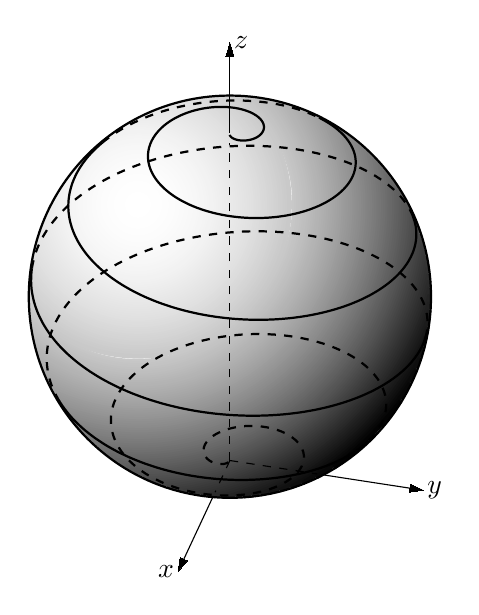
\begin{tikzpicture}[scale=2.54]
% dpic version 2019.06.20 option -g for TikZ and PGF 1.01
\ifx\dpiclw\undefined\newdimen\dpiclw\fi
\global\def\dpicdraw{\draw[line width=\dpiclw]}
\global\def\dpicstop{;}
\dpiclw=0.8bp
\dpiclw=0.8bp
\dpicdraw[line width=1.6bp,draw={rgb,1:red,0.99995;green,0.99995;blue,0.99995}](-0.459619,1.278771) circle (0.004389in)\dpicstop
\dpicdraw[line width=1.6bp,draw={rgb,1:red,0.99982;green,0.99982;blue,0.99982}](-0.459619,1.278771) circle (0.008778in)\dpicstop
\dpicdraw[line width=1.6bp,draw={rgb,1:red,0.99959;green,0.99959;blue,0.99959}](-0.459619,1.278771) circle (0.013168in)\dpicstop
\dpicdraw[line width=1.6bp,draw={rgb,1:red,0.99927;green,0.99927;blue,0.99927}](-0.459619,1.278771) circle (0.017557in)\dpicstop
\dpicdraw[line width=1.6bp,draw={rgb,1:red,0.99886;green,0.99886;blue,0.99886}](-0.459619,1.278771) circle (0.021946in)\dpicstop
\dpicdraw[line width=1.6bp,draw={rgb,1:red,0.99836;green,0.99836;blue,0.99836}](-0.459619,1.278771) circle (0.026335in)\dpicstop
\dpicdraw[line width=1.6bp,draw={rgb,1:red,0.99776;green,0.99776;blue,0.99776}](-0.459619,1.278771) circle (0.030725in)\dpicstop
\dpicdraw[line width=1.6bp,draw={rgb,1:red,0.99708;green,0.99708;blue,0.99708}](-0.459619,1.278771) circle (0.035114in)\dpicstop
\dpicdraw[line width=1.6bp,draw={rgb,1:red,0.99630;green,0.99630;blue,0.99630}](-0.459619,1.278771) circle (0.039503in)\dpicstop
\dpicdraw[line width=1.6bp,draw={rgb,1:red,0.99543;green,0.99543;blue,0.99543}](-0.459619,1.278771) circle (0.043892in)\dpicstop
\dpicdraw[line width=1.6bp,draw={rgb,1:red,0.99448;green,0.99448;blue,0.99448}](-0.459619,1.278771) circle (0.048282in)\dpicstop
\dpicdraw[line width=1.6bp,draw={rgb,1:red,0.99343;green,0.99343;blue,0.99343}](-0.459619,1.278771) circle (0.052671in)\dpicstop
\dpicdraw[line width=1.6bp,draw={rgb,1:red,0.99228;green,0.99228;blue,0.99228}](-0.459619,1.278771) circle (0.05706in)\dpicstop
\dpicdraw[line width=1.6bp,draw={rgb,1:red,0.99105;green,0.99105;blue,0.99105}](-0.459619,1.278771) circle (0.061449in)\dpicstop
\dpicdraw[line width=1.6bp,draw={rgb,1:red,0.98973;green,0.98973;blue,0.98973}](-0.459619,1.278771) circle (0.065838in)\dpicstop
\dpicdraw[line width=1.6bp,draw={rgb,1:red,0.98831;green,0.98831;blue,0.98831}](-0.459619,1.278771) circle (0.070228in)\dpicstop
\dpicdraw[line width=1.6bp,draw={rgb,1:red,0.98681;green,0.98681;blue,0.98681}](-0.459619,1.278771) circle (0.074617in)\dpicstop
\dpicdraw[line width=1.6bp,draw={rgb,1:red,0.98521;green,0.98521;blue,0.98521}](-0.459619,1.278771) circle (0.079006in)\dpicstop
\dpicdraw[line width=1.6bp,draw={rgb,1:red,0.98352;green,0.98352;blue,0.98352}](-0.459619,1.278771) circle (0.083395in)\dpicstop
\dpicdraw[line width=1.6bp,draw={rgb,1:red,0.98174;green,0.98174;blue,0.98174}](-0.459619,1.278771) circle (0.087785in)\dpicstop
\dpicdraw[line width=1.6bp,draw={rgb,1:red,0.97987;green,0.97987;blue,0.97987}](-0.459619,1.278771) circle (0.092174in)\dpicstop
\dpicdraw[line width=1.6bp,draw={rgb,1:red,0.97790;green,0.97790;blue,0.97790}](-0.459619,1.278771) circle (0.096563in)\dpicstop
\dpicdraw[line width=1.6bp,draw={rgb,1:red,0.97585;green,0.97585;blue,0.97585}](-0.459619,1.278771) circle (0.100952in)\dpicstop
\dpicdraw[line width=1.6bp,draw={rgb,1:red,0.97370;green,0.97370;blue,0.97370}](-0.459619,1.278771) circle (0.105342in)\dpicstop
\dpicdraw[line width=1.6bp,draw={rgb,1:red,0.97147;green,0.97147;blue,0.97147}](-0.459619,1.278771) circle (0.109731in)\dpicstop
\dpicdraw[line width=1.6bp,draw={rgb,1:red,0.96914;green,0.96914;blue,0.96914}](-0.459619,1.278771) circle (0.11412in)\dpicstop
\dpicdraw[line width=1.6bp,draw={rgb,1:red,0.96672;green,0.96672;blue,0.96672}](-0.459619,1.278771) circle (0.118509in)\dpicstop
\dpicdraw[line width=1.6bp,draw={rgb,1:red,0.96421;green,0.96421;blue,0.96421}](-0.459619,1.278771) circle (0.122898in)\dpicstop
\dpicdraw[line width=1.6bp,draw={rgb,1:red,0.96161;green,0.96161;blue,0.96161}](-0.459619,1.278771) circle (0.127288in)\dpicstop
\dpicdraw[line width=1.6bp,draw={rgb,1:red,0.95891;green,0.95891;blue,0.95891}](-0.459619,1.278771) circle (0.131677in)\dpicstop
\dpicdraw[line width=1.6bp,draw={rgb,1:red,0.95613;green,0.95613;blue,0.95613}](-0.459619,1.278771) circle (0.136066in)\dpicstop
\dpicdraw[line width=1.6bp,draw={rgb,1:red,0.95325;green,0.95325;blue,0.95325}](-0.643957,1.584214)
 ..controls (-0.283293,1.801877) and (0.090518,1.324378)
 ..(-0.207354,1.026506)
 ..controls (-0.505226,0.728634) and (-0.982725,1.102445)
 ..(-0.765062,1.463109)\dpicstop
\dpicdraw[line width=1.6bp,draw={rgb,1:red,0.95028;green,0.95028;blue,0.95028}](-0.600923,1.618459)
 ..controls (-0.228938,1.773197) and (0.085412,1.303506)
 ..(-0.199471,1.018623)
 ..controls (-0.484354,0.73374) and (-0.954045,1.04809)
 ..(-0.799307,1.420075)\dpicstop
\dpicdraw[line width=1.6bp,draw={rgb,1:red,0.94722;green,0.94722;blue,0.94722}](-0.568459,1.641864)
 ..controls (-0.191286,1.754924) and (0.086838,1.289166)
 ..(-0.191588,1.01074)
 ..controls (-0.470014,0.732314) and (-0.935772,1.010438)
 ..(-0.822712,1.387611)\dpicstop
\dpicdraw[line width=1.6bp,draw={rgb,1:red,0.94407;green,0.94407;blue,0.94407}](-0.540491,1.660502)
 ..controls (-0.160556,1.740993) and (0.090914,1.277475)
 ..(-0.183704,1.002856)
 ..controls (-0.458322,0.728238) and (-0.921841,0.979708)
 ..(-0.841349,1.359644)\dpicstop
\dpicdraw[line width=1.6bp,draw={rgb,1:red,0.94083;green,0.94083;blue,0.94083}](-0.515127,1.676266)
 ..controls (-0.133764,1.729521) and (0.09646,1.267254)
 ..(-0.175821,0.994973)
 ..controls (-0.448102,0.722692) and (-0.910369,0.952916)
 ..(-0.857114,1.334279)\dpicstop
\dpicdraw[line width=1.6bp,draw={rgb,1:red,0.93750;green,0.93750;blue,0.93750}](-0.491484,1.690039)
 ..controls (-0.109548,1.71963) and (0.102941,1.257969)
 ..(-0.167938,0.98709)
 ..controls (-0.438816,0.716211) and (-0.900478,0.9287)
 ..(-0.870887,1.310636)\dpicstop
\dpicdraw[line width=1.6bp,draw={rgb,1:red,0.93408;green,0.93408;blue,0.93408}](-0.469067,1.702315)
 ..controls (-0.087159,1.710833) and (0.110062,1.249324)
 ..(-0.160055,0.979207)
 ..controls (-0.430172,0.70909) and (-0.891681,0.906311)
 ..(-0.883163,1.288219)\dpicstop
\dpicdraw[line width=1.6bp,draw={rgb,1:red,0.93056;green,0.93056;blue,0.93056}](-0.447568,1.713402)
 ..controls (-0.066136,1.702826) and (0.117645,1.24114)
 ..(-0.152171,0.971323)
 ..controls (-0.421988,0.701507) and (-0.883674,0.885289)
 ..(-0.89425,1.266721)\dpicstop
\dpicdraw[line width=1.6bp,draw={rgb,1:red,0.92695;green,0.92695;blue,0.92695}](-0.426782,1.723507)
 ..controls (-0.046179,1.695404) and (0.125572,1.2333)
 ..(-0.144288,0.96344)
 ..controls (-0.414148,0.69358) and (-0.876252,0.865331)
 ..(-0.904355,1.245934)\dpicstop
\dpicdraw[line width=1.6bp,draw={rgb,1:red,0.92326;green,0.92326;blue,0.92326}](-0.40656,1.732776)
 ..controls (-0.027074,1.688426) and (0.133759,1.22572)
 ..(-0.136405,0.955557)
 ..controls (-0.406568,0.685393) and (-0.869274,0.846226)
 ..(-0.913624,1.225712)\dpicstop
\dpicdraw[line width=1.6bp,draw={rgb,1:red,0.91947;green,0.91947;blue,0.91947}](-0.386796,1.741317)
 ..controls (-0.00867,1.681785) and (0.142148,1.218343)
 ..(-0.128521,0.947673)
 ..controls (-0.399191,0.677004) and (-0.862633,0.827822)
 ..(-0.922165,1.205948)\dpicstop
\dpicdraw[line width=1.6bp,draw={rgb,1:red,0.91559;green,0.91559;blue,0.91559}](-0.367409,1.749211)
 ..controls (0.009148,1.675403) and (0.150695,1.211123)
 ..(-0.120638,0.93979)
 ..controls (-0.391971,0.668457) and (-0.856251,0.810004)
 ..(-0.930059,1.186561)\dpicstop
\dpicdraw[line width=1.6bp,draw={rgb,1:red,0.91161;green,0.91161;blue,0.91161}](-0.348335,1.756522)
 ..controls (0.026467,1.669218) and (0.159365,1.204027)
 ..(-0.112755,0.931907)
 ..controls (-0.384875,0.659787) and (-0.850066,0.792685)
 ..(-0.93737,1.167487)\dpicstop
\dpicdraw[line width=1.6bp,draw={rgb,1:red,0.90755;green,0.90755;blue,0.90755}](-0.329524,1.763299)
 ..controls (0.043355,1.663181) and (0.168132,1.197028)
 ..(-0.104872,0.924024)
 ..controls (-0.377876,0.65102) and (-0.844029,0.775797)
 ..(-0.944147,1.148676)\dpicstop
\dpicdraw[line width=1.6bp,draw={rgb,1:red,0.90340;green,0.90340;blue,0.90340}](-0.310936,1.769583)
 ..controls (0.059867,1.657254) and (0.176976,1.190105)
 ..(-0.096988,0.91614)
 ..controls (-0.370953,0.642176) and (-0.838102,0.759285)
 ..(-0.950431,1.130088)\dpicstop
\dpicdraw[line width=1.6bp,draw={rgb,1:red,0.89915;green,0.89915;blue,0.89915}](-0.292538,1.775406)
 ..controls (0.076047,1.651404) and (0.185879,1.183241)
 ..(-0.089105,0.908257)
 ..controls (-0.364089,0.633273) and (-0.832252,0.743105)
 ..(-0.956254,1.11169)\dpicstop
\dpicdraw[line width=1.6bp,draw={rgb,1:red,0.89481;green,0.89481;blue,0.89481}](-0.274304,1.780795)
 ..controls (0.091931,1.645604) and (0.194826,1.176422)
 ..(-0.081222,0.900374)
 ..controls (-0.35727,0.624326) and (-0.826452,0.727221)
 ..(-0.961643,1.093456)\dpicstop
\dpicdraw[line width=1.6bp,draw={rgb,1:red,0.89039;green,0.89039;blue,0.89039}](-0.25621,1.785773)
 ..controls (0.107549,1.639833) and (0.203807,1.169636)
 ..(-0.073338,0.89249)
 ..controls (-0.350484,0.615345) and (-0.820681,0.711603)
 ..(-0.966621,1.075362)\dpicstop
\dpicdraw[line width=1.6bp,draw={rgb,1:red,0.88587;green,0.88587;blue,0.88587}](-0.238239,1.790359)
 ..controls (0.122924,1.634071) and (0.212811,1.162874)
 ..(-0.065455,0.884607)
 ..controls (-0.343722,0.606341) and (-0.814919,0.696228)
 ..(-0.971207,1.057391)\dpicstop
\dpicdraw[line width=1.6bp,draw={rgb,1:red,0.88125;green,0.88125;blue,0.88125}](-0.220373,1.794568)
 ..controls (0.138079,1.628304) and (0.221831,1.156127)
 ..(-0.057572,0.876724)
 ..controls (-0.336975,0.597321) and (-0.809152,0.681073)
 ..(-0.975416,1.039525)\dpicstop
\dpicdraw[line width=1.6bp,draw={rgb,1:red,0.87655;green,0.87655;blue,0.87655}](-0.202601,1.798414)
 ..controls (0.153031,1.622516) and (0.230859,1.149388)
 ..(-0.049689,0.868841)
 ..controls (-0.330236,0.588293) and (-0.803364,0.666121)
 ..(-0.979261,1.021753)\dpicstop
\dpicdraw[line width=1.6bp,draw={rgb,1:red,0.87176;green,0.87176;blue,0.87176}](-0.184909,1.801908)
 ..controls (0.167794,1.616695) and (0.239889,1.142652)
 ..(-0.041805,0.860957)
 ..controls (-0.323499,0.579263) and (-0.797543,0.651358)
 ..(-0.982756,1.004061)\dpicstop
\dpicdraw[line width=1.6bp,draw={rgb,1:red,0.86687;green,0.86687;blue,0.86687}](-0.167289,1.80506)
 ..controls (0.182382,1.610833) and (0.248916,1.135912)
 ..(-0.033922,0.853074)
 ..controls (-0.31676,0.570236) and (-0.791681,0.63677)
 ..(-0.985908,0.986441)\dpicstop
\dpicdraw[line width=1.6bp,draw={rgb,1:red,0.86190;green,0.86190;blue,0.86190}](-0.149732,1.807879)
 ..controls (0.196806,1.604918) and (0.257935,1.129164)
 ..(-0.026039,0.845191)
 ..controls (-0.310012,0.561217) and (-0.785766,0.622346)
 ..(-0.988727,0.968884)\dpicstop
\dpicdraw[line width=1.6bp,draw={rgb,1:red,0.85683;green,0.85683;blue,0.85683}](-0.132231,1.810371)
 ..controls (0.211076,1.598944) and (0.266942,1.122405)
 ..(-0.018155,0.837307)
 ..controls (-0.303253,0.55221) and (-0.779792,0.608076)
 ..(-0.991219,0.951383)\dpicstop
\dpicdraw[line width=1.6bp,draw={rgb,1:red,0.85167;green,0.85167;blue,0.85167}](-0.11478,1.812543)
 ..controls (0.225199,1.592902) and (0.275934,1.11563)
 ..(-0.010272,0.829424)
 ..controls (-0.296478,0.543218) and (-0.77375,0.593953)
 ..(-0.993391,0.933932)\dpicstop
\dpicdraw[line width=1.6bp,draw={rgb,1:red,0.84642;green,0.84642;blue,0.84642}](-0.097374,1.8144)
 ..controls (0.239183,1.586787) and (0.284907,1.108837)
 ..(-0.002389,0.821541)
 ..controls (-0.289685,0.534245) and (-0.767635,0.57997)
 ..(-0.995248,0.916526)\dpicstop
\dpicdraw[line width=1.6bp,draw={rgb,1:red,0.84108;green,0.84108;blue,0.84108}](-0.080008,1.815946)
 ..controls (0.253033,1.580592) and (0.293859,1.102022)
 ..(0.005494,0.813658)
 ..controls (-0.28287,0.525293) and (-0.76144,0.566119)
 ..(-0.996794,0.89916)\dpicstop
\dpicdraw[line width=1.6bp,draw={rgb,1:red,0.83565;green,0.83565;blue,0.83565}](-0.062678,1.817186)
 ..controls (0.266757,1.574313) and (0.302786,1.095183)
 ..(0.013378,0.805774)
 ..controls (-0.276031,0.516366) and (-0.755161,0.552395)
 ..(-0.998034,0.88183)\dpicstop
\dpicdraw[line width=1.6bp,draw={rgb,1:red,0.83012;green,0.83012;blue,0.83012}](-0.045381,1.818122)
 ..controls (0.280358,1.567944) and (0.311687,1.088318)
 ..(0.021261,0.797891)
 ..controls (-0.269165,0.507465) and (-0.748792,0.538794)
 ..(-0.99897,0.864533)\dpicstop
\dpicdraw[line width=1.6bp,draw={rgb,1:red,0.82451;green,0.82451;blue,0.82451}](-0.028115,1.818757)
 ..controls (0.29384,1.561481) and (0.32056,1.081423)
 ..(0.029144,0.790008)
 ..controls (-0.262271,0.498592) and (-0.742329,0.525312)
 ..(-0.999605,0.847267)\dpicstop
\dpicdraw[line width=1.6bp,draw={rgb,1:red,0.81880;green,0.81880;blue,0.81880}](-0.010878,1.819093)
 ..controls (0.307207,1.55492) and (0.329402,1.074499)
 ..(0.037028,0.782124)
 ..controls (-0.255347,0.48975) and (-0.735768,0.511945)
 ..(-0.999941,0.83003)\dpicstop
\dpicdraw[line width=1.6bp,draw={rgb,1:red,0.81300;green,0.81300;blue,0.81300}](0.006333,1.819132)
 ..controls (0.320463,1.548258) and (0.338211,1.067541)
 ..(0.044911,0.774241)
 ..controls (-0.248389,0.480941) and (-0.729106,0.498689)
 ..(-0.99998,0.812819)\dpicstop
\dpicdraw[line width=1.6bp,draw={rgb,1:red,0.80711;green,0.80711;blue,0.80711}](0.023519,1.818875)
 ..controls (0.333609,1.541491) and (0.346986,1.06055)
 ..(0.052794,0.766358)
 ..controls (-0.241398,0.472166) and (-0.722339,0.485543)
 ..(-0.999723,0.795633)\dpicstop
\dpicdraw[line width=1.6bp,draw={rgb,1:red,0.80113;green,0.80113;blue,0.80113}](0.040681,1.818324)
 ..controls (0.346649,1.534615) and (0.355726,1.053523)
 ..(0.060677,0.758475)
 ..controls (-0.234371,0.463426) and (-0.715463,0.472503)
 ..(-0.999172,0.778471)\dpicstop
\dpicdraw[line width=1.6bp,draw={rgb,1:red,0.79506;green,0.79506;blue,0.79506}](0.057819,1.817479)
 ..controls (0.359584,1.527628) and (0.364429,1.046459)
 ..(0.068561,0.750591)
 ..controls (-0.227307,0.454723) and (-0.708476,0.459568)
 ..(-0.998327,0.761333)\dpicstop
\dpicdraw[line width=1.6bp,draw={rgb,1:red,0.78890;green,0.78890;blue,0.78890}](0.074934,1.816341)
 ..controls (0.372416,1.520527) and (0.373093,1.039357)
 ..(0.076444,0.742708)
 ..controls (-0.220205,0.446059) and (-0.701375,0.446736)
 ..(-0.997188,0.744218)\dpicstop
\dpicdraw[line width=1.6bp,draw={rgb,1:red,0.78264;green,0.78264;blue,0.78264}](0.092026,1.814909)
 ..controls (0.796757,1.089793) and (-0.270641,0.022395)
 ..(-0.995757,0.727126)\dpicstop
\dpicdraw[line width=1.6bp,draw={rgb,1:red,0.77630;green,0.77630;blue,0.77630}](0.109095,1.813183)
 ..controls (0.799831,1.07811) and (-0.258958,0.019321)
 ..(-0.994031,0.710057)\dpicstop
\dpicdraw[line width=1.6bp,draw={rgb,1:red,0.76986;green,0.76986;blue,0.76986}](0.126141,1.811164)
 ..controls (0.802926,1.066538) and (-0.247386,0.016226)
 ..(-0.992012,0.693011)\dpicstop
\dpicdraw[line width=1.6bp,draw={rgb,1:red,0.76333;green,0.76333;blue,0.76333}](0.143163,1.808851)
 ..controls (0.806032,1.055067) and (-0.235915,0.01312)
 ..(-0.989699,0.675989)\dpicstop
\dpicdraw[line width=1.6bp,draw={rgb,1:red,0.75671;green,0.75671;blue,0.75671}](0.160161,1.806243)
 ..controls (0.809141,1.043689) and (-0.224537,0.010011)
 ..(-0.987091,0.658991)\dpicstop
\dpicdraw[line width=1.6bp,draw={rgb,1:red,0.75000;green,0.75000;blue,0.75000}](0.177133,1.803339)
 ..controls (0.812247,1.032398) and (-0.213246,0.006905)
 ..(-0.984187,0.642019)\dpicstop
\dpicdraw[line width=1.6bp,draw={rgb,1:red,0.74320;green,0.74320;blue,0.74320}](0.194079,1.800138)
 ..controls (0.815342,1.021187) and (-0.202035,0.00381)
 ..(-0.980986,0.625073)\dpicstop
\dpicdraw[line width=1.6bp,draw={rgb,1:red,0.73630;green,0.73630;blue,0.73630}](0.210997,1.796639)
 ..controls (0.818422,1.01005) and (-0.190898,0.000731)
 ..(-0.977487,0.608155)\dpicstop
\dpicdraw[line width=1.6bp,draw={rgb,1:red,0.72932;green,0.72932;blue,0.72932}](0.227885,1.79284)
 ..controls (0.821479,0.99898) and (-0.179828,-0.002327)
 ..(-0.973688,0.591267)\dpicstop
\dpicdraw[line width=1.6bp,draw={rgb,1:red,0.72224;green,0.72224;blue,0.72224}](0.244743,1.78874)
 ..controls (0.824509,0.987974) and (-0.168822,-0.005357)
 ..(-0.969588,0.574409)\dpicstop
\dpicdraw[line width=1.6bp,draw={rgb,1:red,0.71507;green,0.71507;blue,0.71507}](0.261569,1.784337)
 ..controls (0.827507,0.977027) and (-0.157875,-0.008355)
 ..(-0.965185,0.557583)\dpicstop
\dpicdraw[line width=1.6bp,draw={rgb,1:red,0.70782;green,0.70782;blue,0.70782}](0.278359,1.779629)
 ..controls (0.830469,0.966133) and (-0.146981,-0.011317)
 ..(-0.960477,0.540793)\dpicstop
\dpicdraw[line width=1.6bp,draw={rgb,1:red,0.70047;green,0.70047;blue,0.70047}](0.295114,1.774614)
 ..controls (0.833392,0.95529) and (-0.136138,-0.014239)
 ..(-0.955462,0.524038)\dpicstop
\dpicdraw[line width=1.6bp,draw={rgb,1:red,0.69302;green,0.69302;blue,0.69302}](0.311829,1.76929)
 ..controls (0.83627,0.944492) and (-0.12534,-0.017118)
 ..(-0.950138,0.507323)\dpicstop
\dpicdraw[line width=1.6bp,draw={rgb,1:red,0.68549;green,0.68549;blue,0.68549}](0.328504,1.763655)
 ..controls (0.8391,0.933737) and (-0.114585,-0.019948)
 ..(-0.944503,0.490648)\dpicstop
\dpicdraw[line width=1.6bp,draw={rgb,1:red,0.67787;green,0.67787;blue,0.67787}](0.345135,1.757705)
 ..controls (0.84188,0.923022) and (-0.10387,-0.022728)
 ..(-0.938553,0.474017)\dpicstop
\dpicdraw[line width=1.6bp,draw={rgb,1:red,0.67015;green,0.67015;blue,0.67015}](0.36172,1.751439)
 ..controls (0.844606,0.912343) and (-0.093191,-0.025454)
 ..(-0.932287,0.457432)\dpicstop
\dpicdraw[line width=1.6bp,draw={rgb,1:red,0.66234;green,0.66234;blue,0.66234}](0.378255,1.744853)
 ..controls (0.847275,0.901697) and (-0.082545,-0.028123)
 ..(-0.925701,0.440897)\dpicstop
\dpicdraw[line width=1.6bp,draw={rgb,1:red,0.65445;green,0.65445;blue,0.65445}](0.394739,1.737945)
 ..controls (0.849885,0.891082) and (-0.07193,-0.030733)
 ..(-0.918793,0.424413)\dpicstop
\dpicdraw[line width=1.6bp,draw={rgb,1:red,0.64646;green,0.64646;blue,0.64646}](0.411168,1.730712)
 ..controls (0.852432,0.880494) and (-0.061342,-0.03328)
 ..(-0.91156,0.407984)\dpicstop
\dpicdraw[line width=1.6bp,draw={rgb,1:red,0.63838;green,0.63838;blue,0.63838}](0.427538,1.723149)
 ..controls (0.854915,0.869933) and (-0.050781,-0.035763)
 ..(-0.903997,0.391614)\dpicstop
\dpicdraw[line width=1.6bp,draw={rgb,1:red,0.63020;green,0.63020;blue,0.63020}](0.443846,1.715255)
 ..controls (0.857331,0.859394) and (-0.040242,-0.038179)
 ..(-0.896103,0.375306)\dpicstop
\dpicdraw[line width=1.6bp,draw={rgb,1:red,0.62194;green,0.62194;blue,0.62194}](0.460089,1.707025)
 ..controls (0.859678,0.848876) and (-0.029724,-0.040525)
 ..(-0.887873,0.359063)\dpicstop
\dpicdraw[line width=1.6bp,draw={rgb,1:red,0.61359;green,0.61359;blue,0.61359}](0.476263,1.698455)
 ..controls (0.861953,0.838377) and (-0.019225,-0.042801)
 ..(-0.879303,0.342889)\dpicstop
\dpicdraw[line width=1.6bp,draw={rgb,1:red,0.60514;green,0.60514;blue,0.60514}](0.492364,1.689541)
 ..controls (0.864154,0.827895) and (-0.008743,-0.045002)
 ..(-0.870389,0.326788)\dpicstop
\dpicdraw[line width=1.6bp,draw={rgb,1:red,0.59660;green,0.59660;blue,0.59660}](0.508388,1.68028)
 ..controls (0.866281,0.817428) and (0.001724,-0.047129)
 ..(-0.861128,0.310764)\dpicstop
\dpicdraw[line width=1.6bp,draw={rgb,1:red,0.58797;green,0.58797;blue,0.58797}](0.52433,1.670667)
 ..controls (0.86833,0.806973) and (0.012179,-0.049178)
 ..(-0.851515,0.294822)\dpicstop
\dpicdraw[line width=1.6bp,draw={rgb,1:red,0.57925;green,0.57925;blue,0.57925}](0.540186,1.660698)
 ..controls (0.870299,0.796529) and (0.022623,-0.051147)
 ..(-0.841546,0.278966)\dpicstop
\dpicdraw[line width=1.6bp,draw={rgb,1:red,0.57044;green,0.57044;blue,0.57044}](0.555951,1.650367)
 ..controls (0.872187,0.786094) and (0.033059,-0.053035)
 ..(-0.831215,0.263201)\dpicstop
\dpicdraw[line width=1.6bp,draw={rgb,1:red,0.56154;green,0.56154;blue,0.56154}](0.571621,1.63967)
 ..controls (0.873993,0.775665) and (0.043487,-0.054841)
 ..(-0.820518,0.247531)\dpicstop
\dpicdraw[line width=1.6bp,draw={rgb,1:red,0.55255;green,0.55255;blue,0.55255}](0.587189,1.628602)
 ..controls (0.875713,0.765243) and (0.053909,-0.056561)
 ..(-0.80945,0.231963)\dpicstop
\dpicdraw[line width=1.6bp,draw={rgb,1:red,0.54346;green,0.54346;blue,0.54346}](0.602651,1.617157)
 ..controls (0.877347,0.754823) and (0.064329,-0.058195)
 ..(-0.798005,0.216501)\dpicstop
\dpicdraw[line width=1.6bp,draw={rgb,1:red,0.53429;green,0.53429;blue,0.53429}](0.618001,1.605329)
 ..controls (0.878892,0.744406) and (0.074746,-0.05974)
 ..(-0.786177,0.201151)\dpicstop
\dpicdraw[line width=1.6bp,draw={rgb,1:red,0.52502;green,0.52502;blue,0.52502}](0.633233,1.593113)
 ..controls (0.880347,0.733988) and (0.085164,-0.061195)
 ..(-0.773961,0.185919)\dpicstop
\dpicdraw[line width=1.6bp,draw={rgb,1:red,0.51566;green,0.51566;blue,0.51566}](0.648341,1.580502)
 ..controls (0.88171,0.723568) and (0.095584,-0.062558)
 ..(-0.76135,0.170811)\dpicstop
\dpicdraw[line width=1.6bp,draw={rgb,1:red,0.50621;green,0.50621;blue,0.50621}](0.663318,1.56749)
 ..controls (0.882979,0.713145) and (0.106007,-0.063826)
 ..(-0.748338,0.155834)\dpicstop
\dpicdraw[line width=1.6bp,draw={rgb,1:red,0.49667;green,0.49667;blue,0.49667}](0.678157,1.554069)
 ..controls (0.884152,0.702715) and (0.116437,-0.065)
 ..(-0.734917,0.140995)\dpicstop
\dpicdraw[line width=1.6bp,draw={rgb,1:red,0.48703;green,0.48703;blue,0.48703}](0.69285,1.540233)
 ..controls (0.885227,0.692278) and (0.126874,-0.066075)
 ..(-0.721081,0.126302)\dpicstop
\dpicdraw[line width=1.6bp,draw={rgb,1:red,0.47731;green,0.47731;blue,0.47731}](0.707391,1.525974)
 ..controls (0.886202,0.681832) and (0.13732,-0.06705)
 ..(-0.706822,0.111761)\dpicstop
\dpicdraw[line width=1.6bp,draw={rgb,1:red,0.46749;green,0.46749;blue,0.46749}](0.721771,1.511284)
 ..controls (0.887076,0.671374) and (0.147778,-0.067924)
 ..(-0.692132,0.097381)\dpicstop
\dpicdraw[line width=1.6bp,draw={rgb,1:red,0.45759;green,0.45759;blue,0.45759}](0.735982,1.496153)
 ..controls (0.887846,0.660902) and (0.15825,-0.068694)
 ..(-0.677001,0.08317)\dpicstop
\dpicdraw[line width=1.6bp,draw={rgb,1:red,0.44759;green,0.44759;blue,0.44759}](0.750014,1.480574)
 ..controls (0.888509,0.650414) and (0.168738,-0.069357)
 ..(-0.661422,0.069138)\dpicstop
\dpicdraw[line width=1.6bp,draw={rgb,1:red,0.43750;green,0.43750;blue,0.43750}](0.763858,1.464536)
 ..controls (0.889064,0.639907) and (0.179245,-0.069912)
 ..(-0.645384,0.055294)\dpicstop
\dpicdraw[line width=1.6bp,draw={rgb,1:red,0.42732;green,0.42732;blue,0.42732}](0.777504,1.44803)
 ..controls (0.889509,0.62938) and (0.189772,-0.070357)
 ..(-0.628878,0.041648)\dpicstop
\dpicdraw[line width=1.6bp,draw={rgb,1:red,0.41705;green,0.41705;blue,0.41705}](0.790941,1.431044)
 ..controls (0.889839,0.61883) and (0.200322,-0.070687)
 ..(-0.611892,0.028211)\dpicstop
\dpicdraw[line width=1.6bp,draw={rgb,1:red,0.40668;green,0.40668;blue,0.40668}](0.804158,1.413567)
 ..controls (0.890054,0.608253) and (0.210899,-0.070902)
 ..(-0.594415,0.014994)\dpicstop
\dpicdraw[line width=1.6bp,draw={rgb,1:red,0.39623;green,0.39623;blue,0.39623}](0.817142,1.395588)
 ..controls (0.890149,0.597648) and (0.221504,-0.070997)
 ..(-0.576436,0.00201)\dpicstop
\dpicdraw[line width=1.6bp,draw={rgb,1:red,0.38568;green,0.38568;blue,0.38568}](0.829881,1.377093)
 ..controls (0.890123,0.58701) and (0.232142,-0.070971)
 ..(-0.557941,-0.010729)\dpicstop
\dpicdraw[line width=1.6bp,draw={rgb,1:red,0.37505;green,0.37505;blue,0.37505}](0.84236,1.358067)
 ..controls (0.889971,0.576338) and (0.242814,-0.070818)
 ..(-0.538915,-0.023208)\dpicstop
\dpicdraw[line width=1.6bp,draw={rgb,1:red,0.36432;green,0.36432;blue,0.36432}](0.854565,1.338497)
 ..controls (0.889689,0.565626) and (0.253526,-0.070537)
 ..(-0.519345,-0.035413)\dpicstop
\dpicdraw[line width=1.6bp,draw={rgb,1:red,0.35350;green,0.35350;blue,0.35350}](0.866479,1.318366)
 ..controls (0.889275,0.554871) and (0.264281,-0.070123)
 ..(-0.499214,-0.047327)\dpicstop
\dpicdraw[line width=1.6bp,draw={rgb,1:red,0.34259;green,0.34259;blue,0.34259}](0.878085,1.297656)
 ..controls (0.888724,0.54407) and (0.275082,-0.069572)
 ..(-0.478504,-0.058933)\dpicstop
\dpicdraw[line width=1.6bp,draw={rgb,1:red,0.33158;green,0.33158;blue,0.33158}](0.889365,1.27635)
 ..controls (0.888031,0.533217) and (0.285935,-0.068879)
 ..(-0.457198,-0.070213)\dpicstop
\dpicdraw[line width=1.6bp,draw={rgb,1:red,0.32049;green,0.32049;blue,0.32049}](0.900298,1.254426)
 ..controls (0.887192,0.522308) and (0.296844,-0.06804)
 ..(-0.435274,-0.081146)\dpicstop
\dpicdraw[line width=1.6bp,draw={rgb,1:red,0.30930;green,0.30930;blue,0.30930}](0.910862,1.231863)
 ..controls (0.8862,0.511337) and (0.307816,-0.067048)
 ..(-0.412711,-0.09171)\dpicstop
\dpicdraw[line width=1.6bp,draw={rgb,1:red,0.29803;green,0.29803;blue,0.29803}](0.921033,1.208637)
 ..controls (0.885051,0.500297) and (0.318855,-0.065899)
 ..(-0.389485,-0.101881)\dpicstop
\dpicdraw[line width=1.6bp,draw={rgb,1:red,0.28666;green,0.28666;blue,0.28666}](0.930784,1.184721)
 ..controls (0.883736,0.489184) and (0.329968,-0.064584)
 ..(-0.365569,-0.111632)\dpicstop
\dpicdraw[line width=1.6bp,draw={rgb,1:red,0.27520;green,0.27520;blue,0.27520}](0.940087,1.160085)
 ..controls (0.88225,0.477988) and (0.341164,-0.063098)
 ..(-0.340933,-0.120935)\dpicstop
\dpicdraw[line width=1.6bp,draw={rgb,1:red,0.26365;green,0.26365;blue,0.26365}](0.94891,1.134699)
 ..controls (0.880583,0.466702) and (0.35245,-0.061431)
 ..(-0.315547,-0.129758)\dpicstop
\dpicdraw[line width=1.6bp,draw={rgb,1:red,0.25201;green,0.25201;blue,0.25201}](0.957216,1.108526)
 ..controls (0.878727,0.455317) and (0.363835,-0.059575)
 ..(-0.289374,-0.138064)\dpicstop
\dpicdraw[line width=1.6bp,draw={rgb,1:red,0.24028;green,0.24028;blue,0.24028}](0.964966,1.081527)
 ..controls (0.876671,0.443822) and (0.37533,-0.057519)
 ..(-0.262375,-0.145814)\dpicstop
\dpicdraw[line width=1.6bp,draw={rgb,1:red,0.22845;green,0.22845;blue,0.22845}](0.972115,1.053656)
 ..controls (0.874403,0.432205) and (0.386947,-0.055251)
 ..(-0.234504,-0.152963)\dpicstop
\dpicdraw[line width=1.6bp,draw={rgb,1:red,0.21654;green,0.21654;blue,0.21654}](0.978613,1.024863)
 ..controls (0.871909,0.420452) and (0.3987,-0.052757)
 ..(-0.205711,-0.159461)\dpicstop
\dpicdraw[line width=1.6bp,draw={rgb,1:red,0.20453;green,0.20453;blue,0.20453}](0.984401,0.995091)
 ..controls (0.869174,0.408549) and (0.410603,-0.050022)
 ..(-0.175939,-0.165249)\dpicstop
\dpicdraw[line width=1.6bp,draw={rgb,1:red,0.19243;green,0.19243;blue,0.19243}](0.989414,0.964272)
 ..controls (0.866179,0.396476) and (0.422676,-0.047027)
 ..(-0.14512,-0.170262)\dpicstop
\dpicdraw[line width=1.6bp,draw={rgb,1:red,0.18024;green,0.18024;blue,0.18024}](0.993575,0.932331)
 ..controls (0.862903,0.384212) and (0.43494,-0.043751)
 ..(-0.113179,-0.174423)\dpicstop
\dpicdraw[line width=1.6bp,draw={rgb,1:red,0.16796;green,0.16796;blue,0.16796}](0.996793,0.899177)
 ..controls (0.859321,0.371732) and (0.44742,-0.040169)
 ..(-0.080025,-0.177641)\dpicstop
\dpicdraw[line width=1.6bp,draw={rgb,1:red,0.15559;green,0.15559;blue,0.15559}](0.998962,0.864704)
 ..controls (0.855402,0.359005) and (0.460147,-0.03625)
 ..(-0.045552,-0.17981)\dpicstop
\dpicdraw[line width=1.6bp,draw={rgb,1:red,0.14312;green,0.14312;blue,0.14312}](0.999954,0.828783)
 ..controls (0.851109,0.345994) and (0.473158,-0.031957)
 ..(-0.009631,-0.180802)\dpicstop
\dpicdraw[line width=1.6bp,draw={rgb,1:red,0.13057;green,0.13057;blue,0.13057}](0.999611,0.791256)
 ..controls (0.846396,0.332653) and (0.486499,-0.027244)
 ..(0.027896,-0.180459)\dpicstop
\dpicdraw[line width=1.6bp,draw={rgb,1:red,0.11792;green,0.11792;blue,0.11792}](0.997738,0.75193)
 ..controls (0.841204,0.318924) and (0.500228,-0.022052)
 ..(0.067222,-0.178586)\dpicstop
\dpicdraw[line width=1.6bp,draw={rgb,1:red,0.10519;green,0.10519;blue,0.10519}](0.994086,0.710553)
 ..controls (0.83546,0.304732) and (0.51442,-0.016308)
 ..(0.108599,-0.174934)\dpicstop
\dpicdraw[line width=1.6bp,draw={rgb,1:red,0.09236;green,0.09236;blue,0.09236}](0.988326,0.666799)
 ..controls (0.829063,0.289978) and (0.529174,-0.009911)
 ..(0.152353,-0.169174)\dpicstop
\dpicdraw[line width=1.6bp,draw={rgb,1:red,0.07944;green,0.07944;blue,0.07944}](0.980014,0.620221)
 ..controls (0.821877,0.274525) and (0.544627,-0.002725)
 ..(0.198931,-0.160862)\dpicstop
\dpicdraw[line width=1.6bp,draw={rgb,1:red,0.06643;green,0.06643;blue,0.06643}](0.968512,0.570184)
 ..controls (0.813704,0.258175) and (0.560977,0.005448)
 ..(0.248968,-0.14936)\dpicstop
\dpicdraw[line width=1.6bp,draw={rgb,1:red,0.05332;green,0.05332;blue,0.05332}](0.952853,0.515719)
 ..controls (0.804239,0.240624) and (0.578528,0.014913)
 ..(0.303433,-0.133701)\dpicstop
\dpicdraw[line width=1.6bp,draw={rgb,1:red,0.04013;green,0.04013;blue,0.04013}](0.931423,0.455213)
 ..controls (0.79297,0.221358) and (0.597794,0.026182)
 ..(0.363939,-0.112271)\dpicstop
\dpicdraw[line width=1.6bp,draw={rgb,1:red,0.02684;green,0.02684;blue,0.02684}](0.901102,0.385546)
 ..controls (0.778892,0.199373) and (0.619779,0.04026)
 ..(0.433606,-0.08195)\dpicstop
\dpicdraw[line width=1.6bp,draw={rgb,1:red,0.01347;green,0.01347;blue,0.01347}](0.853917,0.298744)
 ..controls (0.75941,0.172075) and (0.647077,0.059742)
 ..(0.520409,-0.034765)\dpicstop
\dpicdraw[line width=1.6bp,draw={rgb,1:red,0.00000;green,0.00000;blue,0.00000}](0.707107,0.112045)
 ..controls (0.707107,0.112045) and (0.707107,0.112045)
 ..(0.707107,0.112045)\dpicstop
\dpicdraw (0,0.819152) circle (0.395888in)\dpicstop
\dpicdraw[dashed](-0.007923,-0.008794)
 ..controls (-0.008878,-0.009374) and (-0.01061,-0.01038)
 ..(-0.011789,-0.011039)
 ..controls (-0.012967,-0.011699) and (-0.015095,-0.012699)
 ..(-0.016536,-0.013271)
 ..controls (-0.017978,-0.013843) and (-0.020724,-0.014729)
 ..(-0.022663,-0.015247)
 ..controls (-0.024602,-0.015765) and (-0.027919,-0.016458)
 ..(-0.030064,-0.016794)
 ..controls (-0.032209,-0.017129) and (-0.035829,-0.017514)
 ..(-0.03814,-0.017653)
 ..controls (-0.040451,-0.017791) and (-0.044308,-0.017845)
 ..(-0.046746,-0.017773)
 ..controls (-0.049183,-0.017702) and (-0.053209,-0.017406)
 ..(-0.055728,-0.017113)
 ..controls (-0.058247,-0.016821) and (-0.06237,-0.016161)
 ..(-0.064925,-0.01564)
 ..controls (-0.067481,-0.01512) and (-0.071624,-0.014086)
 ..(-0.07417,-0.013334)
 ..controls (-0.076715,-0.012581) and (-0.080802,-0.011169)
 ..(-0.083288,-0.010183)
 ..controls (-0.085774,-0.009197) and (-0.089726,-0.007407)
 ..(-0.092105,-0.006189)
 ..controls (-0.094484,-0.004972) and (-0.098223,-0.00281)
 ..(-0.100447,-0.001366)
 ..controls (-0.102671,0.000078) and (-0.106119,0.002601)
 ..(-0.10814,0.004263)
 ..controls (-0.110161,0.005925) and (-0.113242,0.008793)
 ..(-0.115015,0.010662)
 ..controls (-0.116787,0.012531) and (-0.11943,0.015723)
 ..(-0.12091,0.017784)
 ..controls (-0.12239,0.019845) and (-0.124524,0.023336)
 ..(-0.12567,0.025572)
 ..controls (-0.126817,0.027808) and (-0.128378,0.031567)
 ..(-0.129153,0.033958)
 ..controls (-0.129929,0.036349) and (-0.130858,0.040341)
 ..(-0.131227,0.042865)
 ..controls (-0.131597,0.045388) and (-0.131842,0.049575)
 ..(-0.131776,0.052206)
 ..controls (-0.131709,0.054837) and (-0.131225,0.059177)
 ..(-0.130697,0.061889)
 ..controls (-0.130169,0.0646) and (-0.128919,0.069047)
 ..(-0.127908,0.07181)
 ..controls (-0.126897,0.074573) and (-0.124852,0.07908)
 ..(-0.123344,0.081865)
 ..controls (-0.121836,0.084649) and (-0.118974,0.089165)
 ..(-0.116959,0.091939)
 ..controls (-0.114944,0.094714) and (-0.111255,0.099187)
 ..(-0.10873,0.10192)
 ..controls (-0.106204,0.104652) and (-0.101688,0.10903)
 ..(-0.098654,0.111687)
 ..controls (-0.095619,0.114344) and (-0.090284,0.118573)
 ..(-0.08675,0.121123)
 ..controls (-0.083216,0.123672) and (-0.07708,0.127699)
 ..(-0.073061,0.130108)
 ..controls (-0.069042,0.132516) and (-0.062135,0.136289)
 ..(-0.057651,0.138526)
 ..controls (-0.053167,0.140762) and (-0.045528,0.144229)
 ..(-0.040606,0.146262)
 ..controls (-0.035685,0.148294) and (-0.027361,0.151407)
 ..(-0.022036,0.153206)
 ..controls (-0.01671,0.155005) and (-0.00776,0.157716)
 ..(-0.002068,0.159254)
 ..controls (0.003624,0.160793) and (0.013133,0.163058)
 ..(0.019147,0.16431)
 ..controls (0.025161,0.165561) and (0.035154,0.167341)
 ..(0.041441,0.168282)
 ..controls (0.047728,0.169223) and (0.058121,0.170482)
 ..(0.064627,0.171092)
 ..controls (0.071134,0.171701) and (0.081836,0.172408)
 ..(0.088504,0.172669)
 ..controls (0.095172,0.17293) and (0.106087,0.173058)
 ..(0.112855,0.172955)
 ..controls (0.119623,0.172853) and (0.130647,0.172382)
 ..(0.137451,0.171905)
 ..controls (0.144254,0.171428) and (0.155281,0.170343)
 ..(0.162053,0.169485)
 ..controls (0.168824,0.168626) and (0.179743,0.166918)
 ..(0.186414,0.165675)
 ..controls (0.193084,0.164431) and (0.203782,0.162098)
 ..(0.210281,0.16047)
 ..controls (0.216781,0.158842) and (0.227143,0.155888)
 ..(0.2334,0.15388)
 ..controls (0.239657,0.151872) and (0.249569,0.148308)
 ..(0.255514,0.145929)
 ..controls (0.261458,0.143549) and (0.270806,0.139393)
 ..(0.276368,0.136655)
 ..controls (0.281931,0.133918) and (0.290602,0.129193)
 ..(0.295714,0.126114)
 ..controls (0.300826,0.123035) and (0.308713,0.117773)
 ..(0.31331,0.114374)
 ..controls (0.317906,0.110975) and (0.324904,0.105213)
 ..(0.328922,0.101518)
 ..controls (0.332941,0.097823) and (0.338951,0.091604)
 ..(0.342333,0.087643)
 ..controls (0.345714,0.083682) and (0.350646,0.077056)
 ..(0.353337,0.07286)
 ..controls (0.356027,0.068664) and (0.359796,0.061686)
 ..(0.361746,0.057291)
 ..controls (0.363696,0.052896) and (0.366228,0.045626)
 ..(0.367394,0.041071)
 ..controls (0.36856,0.036515) and (0.369788,0.029018)
 ..(0.370134,0.024344)
 ..controls (0.370479,0.01967) and (0.370349,0.012015)
 ..(0.369843,0.007265)
 ..controls (0.369338,0.002515) and (0.367805,-0.005225)
 ..(0.366425,-0.010004)
 ..controls (0.365045,-0.014783) and (0.36208,-0.022533)
 ..(0.359809,-0.027294)
 ..controls (0.357539,-0.032056) and (0.353121,-0.039737)
 ..(0.349953,-0.044432)
 ..controls (0.346785,-0.049127) and (0.340909,-0.05666)
 ..(0.336844,-0.061239)
 ..controls (0.332778,-0.065818) and (0.325452,-0.073122)
 ..(0.320498,-0.077535)
 ..controls (0.315544,-0.081948) and (0.306788,-0.088943)
 ..(0.300962,-0.093141)
 ..controls (0.295137,-0.097339) and (0.284986,-0.103945)
 ..(0.278315,-0.107879)
 ..controls (0.271644,-0.111812) and (0.260146,-0.117949)
 ..(0.252664,-0.121571)
 ..controls (0.245181,-0.125192) and (0.232399,-0.130785)
 ..(0.224147,-0.134047)
 ..controls (0.215895,-0.13731) and (0.201904,-0.142284)
 ..(0.192933,-0.145144)
 ..controls (0.183962,-0.148003) and (0.16885,-0.152288)
 ..(0.159217,-0.154703)
 ..controls (0.149585,-0.157118) and (0.133452,-0.160648)
 ..(0.123224,-0.162579)
 ..controls (0.112996,-0.164509) and (0.095954,-0.167224)
 ..(0.085203,-0.168635)
 ..controls (0.074451,-0.170046) and (0.056623,-0.171891)
 ..(0.045427,-0.17275)
 ..controls (0.034231,-0.173609) and (0.015748,-0.174535)
 ..(0.004192,-0.174814)
 ..controls (-0.007365,-0.175094) and (-0.02636,-0.175058)
 ..(-0.038187,-0.174735)
 ..controls (-0.050015,-0.174411) and (-0.069374,-0.17338)
 ..(-0.081378,-0.172435)
 ..controls (-0.093382,-0.171489) and (-0.112949,-0.169437)
 ..(-0.125032,-0.167855)
 ..controls (-0.137116,-0.166274) and (-0.15673,-0.163182)
 ..(-0.168792,-0.160956)
 ..controls (-0.180854,-0.15873) and (-0.20035,-0.154588)
 ..(-0.212289,-0.151714)
 ..controls (-0.224228,-0.148841) and (-0.243439,-0.143648)
 ..(-0.25515,-0.140129)
 ..controls (-0.266861,-0.13661) and (-0.285619,-0.130375)
 ..(-0.296999,-0.126218)
 ..controls (-0.30838,-0.122061) and (-0.326516,-0.114801)
 ..(-0.337462,-0.11002)
 ..controls (-0.348409,-0.105239) and (-0.365757,-0.09698)
 ..(-0.376168,-0.091594)
 ..controls (-0.386579,-0.086208) and (-0.402978,-0.076985)
 ..(-0.412754,-0.071019)
 ..controls (-0.422531,-0.065052) and (-0.437822,-0.054911)
 ..(-0.446869,-0.048393)
 ..controls (-0.455916,-0.041876) and (-0.469948,-0.030869)
 ..(-0.478174,-0.023836)
 ..controls (-0.486401,-0.016803) and (-0.49903,-0.004991)
 ..(-0.50635,0.002517)
 ..controls (-0.513671,0.010025) and (-0.524763,0.022572)
 ..(-0.531098,0.03051)
 ..controls (-0.537433,0.038449) and (-0.546865,0.051654)
 ..(-0.552141,0.059973)
 ..controls (-0.557418,0.068292) and (-0.565078,0.082073)
 ..(-0.569231,0.090719)
 ..controls (-0.573384,0.099365) and (-0.579173,0.11363)
 ..(-0.582147,0.122546)
 ..controls (-0.58512,0.131462) and (-0.588954,0.146117)
 ..(-0.5907,0.155243)
 ..controls (-0.592446,0.164368) and (-0.594255,0.179312)
 ..(-0.594736,0.188583)
 ..controls (-0.595216,0.197854) and (-0.594947,0.212982)
 ..(-0.594134,0.222334)
 ..controls (-0.593321,0.231686) and (-0.590936,0.24689)
 ..(-0.588812,0.256255)
 ..controls (-0.586688,0.26562) and (-0.582167,0.28079)
 ..(-0.578726,0.2901)
 ..controls (-0.575284,0.29941) and (-0.568626,0.314434)
 ..(-0.563871,0.323619)
 ..controls (-0.559116,0.332805) and (-0.550336,0.347571)
 ..(-0.544282,0.356563)
 ..controls (-0.538228,0.365554) and (-0.527361,0.37995)
 ..(-0.520035,0.38868)
 ..controls (-0.51271,0.397409) and (-0.499806,0.411324)
 ..(-0.491246,0.419724)
 ..controls (-0.482686,0.428124) and (-0.467817,0.44145)
 ..(-0.458071,0.449455)
 ..controls (-0.448325,0.45746) and (-0.431577,0.470092)
 ..(-0.420704,0.477638)
 ..controls (-0.409832,0.485184) and (-0.391309,0.497021)
 ..(-0.379379,0.504048)
 ..controls (-0.367449,0.511075) and (-0.347273,0.522023)
 ..(-0.334365,0.528473)
 ..controls (-0.321458,0.534924) and (-0.299765,0.544892)
 ..(-0.285968,0.550714)
 ..controls (-0.272171,0.556535) and (-0.249112,0.565441)
 ..(-0.234523,0.570585)
 ..controls (-0.219934,0.575728) and (-0.195676,0.583498)
 ..(-0.1804,0.58792)
 ..controls (-0.165125,0.592342) and (-0.139842,0.598909)
 ..(-0.123993,0.602572)
 ..controls (-0.108144,0.606234) and (-0.082026,0.611541)
 ..(-0.065722,0.614411)
 ..controls (-0.049419,0.617282) and (-0.022664,0.621281)
 ..(-0.00603,0.623333)
 ..controls (0.010604,0.625386) and (0.037791,0.628039)
 ..(0.054625,0.629254)
 ..controls (0.07146,0.630468) and (0.098866,0.63175)
 ..(0.115769,0.632114)
 ..controls (0.132672,0.632477) and (0.16008,0.632372)
 ..(0.176917,0.631878)
 ..controls (0.193754,0.631385) and (0.220942,0.629887)
 ..(0.237577,0.628538)
 ..controls (0.254211,0.627188) and (0.28096,0.624306)
 ..(0.297256,0.622108)
 ..controls (0.313551,0.61991) and (0.33964,0.615663)
 ..(0.355461,0.612632)
 ..controls (0.371282,0.6096) and (0.396492,0.604017)
 ..(0.411706,0.600176)
 ..controls (0.42692,0.596334) and (0.451037,0.589457)
 ..(0.465513,0.584833)
 ..controls (0.47999,0.58021) and (0.502807,0.572093)
 ..(0.51642,0.566723)
 ..controls (0.530033,0.561354) and (0.55135,0.552061)
 ..(0.56398,0.545988)
 ..controls (0.57661,0.539916) and (0.596238,0.52952)
 ..(0.607771,0.522794)
 ..controls (0.619304,0.516068) and (0.637063,0.504655)
 ..(0.647394,0.49733)
 ..controls (0.657724,0.490005) and (0.67345,0.477667)
 ..(0.68248,0.469804)
 ..controls (0.69151,0.461941) and (0.705052,0.448782)
 ..(0.712693,0.440446)
 ..controls (0.720334,0.432111) and (0.731558,0.418242)
 ..(0.737733,0.409504)
 ..controls (0.743908,0.400766) and (0.752695,0.386304)
 ..(0.757337,0.377239)
 ..controls (0.761979,0.368174) and (0.768231,0.353244)
 ..(0.771285,0.343929)
 ..controls (0.774339,0.334614) and (0.777976,0.319345)
 ..(0.779399,0.309862)
 ..controls (0.780822,0.30038) and (0.781785,0.284905)
 ..(0.781547,0.275337)
 ..controls (0.781309,0.265769) and (0.779561,0.250228)
 ..(0.777647,0.240663)
 ..controls (0.775734,0.231098) and (0.771248,0.215617)
 ..(0.767639,0.206124)
 ..controls (0.76403,0.196631) and (0.756875,0.181418)
 ..(0.751675,0.172182)
 ..controls (0.746475,0.162947) and (0.737238,0.148955)
 ..(0.731066,0.140965)
 ..controls (0.724895,0.132975) and (0.715645,0.121949)
 ..(0.71043,0.116365)
 ..controls (0.705215,0.110781) and (0.697514,0.102752)
 ..(0.693248,0.098453)\dpicstop
\dpicdraw (0.693248,0.098453)
 ..controls (0.692658,0.097794) and (0.690274,0.09553)
 ..(0.687929,0.0934)
 ..controls (0.685584,0.091271) and (0.675865,0.082956)
 ..(0.666244,0.074849)
 ..controls (0.656624,0.066742) and (0.639584,0.054029)
 ..(0.628228,0.046485)
 ..controls (0.616871,0.038942) and (0.597053,0.026943)
 ..(0.584012,0.019716)
 ..controls (0.570971,0.012489) and (0.548741,0.001319)
 ..(0.534415,-0.005205)
 ..controls (0.520088,-0.011728) and (0.495807,-0.021744)
 ..(0.480242,-0.02755)
 ..controls (0.464677,-0.033356) and (0.438481,-0.042146)
 ..(0.421797,-0.047161)
 ..controls (0.405113,-0.052176) and (0.377197,-0.059635)
 ..(0.359514,-0.063803)
 ..controls (0.341832,-0.067971) and (0.312398,-0.074012)
 ..(0.293847,-0.077281)
 ..controls (0.275296,-0.08055) and (0.244564,-0.085095)
 ..(0.225282,-0.08742)
 ..controls (0.206,-0.089745) and (0.1742,-0.092725)
 ..(0.154333,-0.094069)
 ..controls (0.134467,-0.095412) and (0.101839,-0.096773)
 ..(0.081539,-0.097105)
 ..controls (0.061239,-0.097437) and (0.028034,-0.097136)
 ..(0.007457,-0.096433)
 ..controls (-0.01312,-0.095731) and (-0.046646,-0.093737)
 ..(-0.067341,-0.091986)
 ..controls (-0.088035,-0.090235) and (-0.12162,-0.086533)
 ..(-0.142271,-0.083726)
 ..controls (-0.162921,-0.08092) and (-0.196301,-0.075506)
 ..(-0.216744,-0.071647)
 ..controls (-0.237187,-0.067788) and (-0.270098,-0.060672)
 ..(-0.290171,-0.055771)
 ..controls (-0.310244,-0.05087) and (-0.342423,-0.042077)
 ..(-0.361965,-0.036152)
 ..controls (-0.381507,-0.030228) and (-0.412695,-0.019794)
 ..(-0.431548,-0.012874)
 ..controls (-0.450401,-0.005953) and (-0.480345,0.00607)
 ..(-0.498356,0.013951)
 ..controls (-0.516366,0.021832) and (-0.544821,0.03538)
 ..(-0.56184,0.044179)
 ..controls (-0.57886,0.052977) and (-0.605591,0.067975)
 ..(-0.621479,0.077641)
 ..controls (-0.637367,0.087306) and (-0.662149,0.103662)
 ..(-0.676769,0.114131)
 ..controls (-0.691388,0.124601) and (-0.714025,0.142234)
 ..(-0.727272,0.153472)
 ..controls (-0.740519,0.16471) and (-0.760741,0.183396)
 ..(-0.772389,0.195161)
 ..controls (-0.784036,0.206925) and (-0.800765,0.225534)
 ..(-0.809711,0.236678)
 ..controls (-0.818657,0.247822) and (-0.830273,0.263231)
 ..(-0.835627,0.271057)
 ..controls (-0.840981,0.278882) and (-0.848476,0.290143)
 ..(-0.852349,0.296179)\dpicstop
\dpicdraw[dashed](-0.852349,0.296179)
 ..controls (-0.853276,0.297545) and (-0.855745,0.301657)
 ..(-0.857859,0.305353)
 ..controls (-0.859973,0.309049) and (-0.867082,0.322546)
 ..(-0.87372,0.335466)
 ..controls (-0.880359,0.348385) and (-0.889493,0.369792)
 ..(-0.894099,0.383225)
 ..controls (-0.898705,0.396659) and (-0.904853,0.418988)
 ..(-0.907815,0.433042)
 ..controls (-0.910778,0.447097) and (-0.913994,0.469995)
 ..(-0.914991,0.484128)
 ..controls (-0.915988,0.498262) and (-0.916035,0.521271)
 ..(-0.915096,0.535462)
 ..controls (-0.914157,0.549654) and (-0.911049,0.572665)
 ..(-0.90816,0.586801)
 ..controls (-0.905272,0.600938) and (-0.899007,0.623781)
 ..(-0.894182,0.637766)
 ..controls (-0.889357,0.651751) and (-0.879965,0.674267)
 ..(-0.873229,0.688001)
 ..controls (-0.866493,0.701735) and (-0.854031,0.723765)
 ..(-0.845425,0.737152)
 ..controls (-0.83682,0.750538) and (-0.821367,0.771926)
 ..(-0.810948,0.784869)
 ..controls (-0.80053,0.797813) and (-0.78219,0.818407)
 ..(-0.77003,0.830816)
 ..controls (-0.75787,0.843224) and (-0.736771,0.862878)
 ..(-0.722955,0.874665)
 ..controls (-0.70914,0.886451) and (-0.68543,0.905025)
 ..(-0.670058,0.916106)
 ..controls (-0.654686,0.927186) and (-0.628539,0.944549)
 ..(-0.611722,0.954845)
 ..controls (-0.594905,0.96514) and (-0.566512,0.98117)
 ..(-0.548374,0.990609)
 ..controls (-0.530237,1.000047) and (-0.499807,1.014631)
 ..(-0.480484,1.023147)
 ..controls (-0.461161,1.031662) and (-0.428924,1.044699)
 ..(-0.408561,1.052232)
 ..controls (-0.388197,1.059766) and (-0.354395,1.071165)
 ..(-0.333145,1.077665)
 ..controls (-0.311896,1.084165) and (-0.276785,1.09385)
 ..(-0.254811,1.099273)
 ..controls (-0.232837,1.104696) and (-0.196686,1.112603)
 ..(-0.174156,1.116914)
 ..controls (-0.151626,1.121225) and (-0.114712,1.127304)
 ..(-0.091799,1.130477)
 ..controls (-0.068886,1.13365) and (-0.031495,1.137865)
 ..(-0.008376,1.139882)
 ..controls (0.014742,1.141898) and (0.052322,1.144229)
 ..(0.075467,1.145081)
 ..controls (0.098611,1.145934) and (0.136087,1.146373)
 ..(0.159077,1.146062)
 ..controls (0.182067,1.145751) and (0.219145,1.144309)
 ..(0.241801,1.142845)
 ..controls (0.264457,1.14138) and (0.300848,1.13808)
 ..(0.322991,1.135481)
 ..controls (0.345135,1.132883) and (0.380551,1.127763)
 ..(0.402007,1.124059)
 ..controls (0.423464,1.120354) and (0.457626,1.113468)
 ..(0.478226,1.108695)
 ..controls (0.498826,1.103922) and (0.531464,1.095337)
 ..(0.551043,1.089541)
 ..controls (0.570623,1.083745) and (0.601476,1.073542)
 ..(0.619879,1.066778)
 ..controls (0.638282,1.060013) and (0.667105,1.048287)
 ..(0.684184,1.040615)
 ..controls (0.701263,1.032944) and (0.727824,1.0198)
 ..(0.743442,1.011291)
 ..controls (0.759061,1.002782) and (0.783145,0.988339)
 ..(0.797176,0.979069)
 ..controls (0.811207,0.969798) and (0.83262,0.954186)
 ..(0.84495,0.944236)
 ..controls (0.85728,0.934286) and (0.875848,0.917642)
 ..(0.886375,0.907102)
 ..controls (0.896903,0.896561) and (0.912472,0.879031)
 ..(0.921111,0.867992)
 ..controls (0.92975,0.856953) and (0.942191,0.838695)
 ..(0.948869,0.827258)
 ..controls (0.955546,0.815821) and (0.964754,0.796981)
 ..(0.969411,0.785224)
 ..controls (0.974068,0.773467) and (0.979971,0.754299)
 ..(0.982581,0.742458)
 ..controls (0.985191,0.730617) and (0.987623,0.712367)
 ..(0.988008,0.701742)
 ..controls (0.988393,0.691117) and (0.988105,0.676231)
 ..(0.987366,0.668531)
 ..controls (0.986626,0.660831) and (0.985336,0.649698)
 ..(0.984487,0.643693)\dpicstop
\dpicdraw (0.984487,0.643693)
 ..controls (0.984437,0.642855) and (0.98386,0.639779)
 ..(0.9832,0.63683)
 ..controls (0.98254,0.633882) and (0.979316,0.622064)
 ..(0.976007,0.610463)
 ..controls (0.972698,0.598862) and (0.965396,0.580217)
 ..(0.959716,0.568864)
 ..controls (0.954035,0.55751) and (0.943124,0.53903)
 ..(0.935372,0.527634)
 ..controls (0.927619,0.516237) and (0.913437,0.498123)
 ..(0.903729,0.487221)
 ..controls (0.894022,0.476319) and (0.876714,0.459027)
 ..(0.865113,0.448642)
 ..controls (0.853513,0.438257) and (0.833201,0.421894)
 ..(0.819797,0.412134)
 ..controls (0.806393,0.402374) and (0.783233,0.387096)
 ..(0.768125,0.378048)
 ..controls (0.753018,0.369) and (0.727185,0.354947)
 ..(0.710491,0.346695)
 ..controls (0.693796,0.338444) and (0.665488,0.325748)
 ..(0.647333,0.31837)
 ..controls (0.629178,0.310992) and (0.598612,0.299774)
 ..(0.579137,0.293342)
 ..controls (0.559662,0.286909) and (0.527072,0.277278)
 ..(0.506427,0.271854)
 ..controls (0.485782,0.266431) and (0.45142,0.258484)
 ..(0.429764,0.254124)
 ..controls (0.408108,0.249765) and (0.37224,0.243586)
 ..(0.34974,0.240339)
 ..controls (0.327241,0.237092) and (0.290144,0.232751)
 ..(0.266975,0.230654)
 ..controls (0.243806,0.228558) and (0.205769,0.22611)
 ..(0.18211,0.225194)
 ..controls (0.158452,0.224278) and (0.119768,0.223765)
 ..(0.095803,0.22405)
 ..controls (0.071839,0.224335) and (0.032809,0.225782)
 ..(0.008724,0.227278)
 ..controls (-0.01536,0.228775) and (-0.054433,0.232192)
 ..(-0.07845,0.234901)
 ..controls (-0.102467,0.237611) and (-0.141279,0.242993)
 ..(-0.165042,0.246908)
 ..controls (-0.188805,0.250823) and (-0.227055,0.258148)
 ..(-0.25038,0.26325)
 ..controls (-0.273705,0.268353) and (-0.311095,0.277585)
 ..(-0.3338,0.283848)
 ..controls (-0.356505,0.290111) and (-0.392745,0.3012)
 ..(-0.414653,0.308588)
 ..controls (-0.436562,0.315976) and (-0.471371,0.328855)
 ..(-0.492314,0.337322)
 ..controls (-0.513257,0.345789) and (-0.546364,0.360379)
 ..(-0.566178,0.369872)
 ..controls (-0.585993,0.379366) and (-0.617142,0.395573)
 ..(-0.635674,0.406031)
 ..controls (-0.654207,0.416489) and (-0.683157,0.434207)
 ..(-0.700264,0.445561)
 ..controls (-0.717371,0.456915) and (-0.743899,0.476026)
 ..(-0.759449,0.488199)
 ..controls (-0.774998,0.500373) and (-0.798899,0.520748)
 ..(-0.812772,0.533659)
 ..controls (-0.826645,0.546569) and (-0.847735,0.568071)
 ..(-0.859825,0.58163)
 ..controls (-0.871915,0.59519) and (-0.890032,0.61767)
 ..(-0.900247,0.631784)
 ..controls (-0.910461,0.645899) and (-0.925469,0.669203)
 ..(-0.93373,0.683778)
 ..controls (-0.941992,0.698352) and (-0.953777,0.722312)
 ..(-0.960025,0.737235)
 ..controls (-0.966273,0.752158) and (-0.974743,0.776647)
 ..(-0.978924,0.791873)
 ..controls (-0.983104,0.807098) and (-0.988229,0.83172)
 ..(-0.990358,0.846805)
 ..controls (-0.992487,0.861891) and (-0.994076,0.885661)
 ..(-0.993903,0.899838)
 ..controls (-0.99373,0.914015) and (-0.99305,0.931378)
 ..(-0.992387,0.938576)
 ..controls (-0.991724,0.945774) and (-0.990649,0.955512)
 ..(-0.989988,0.960303)\dpicstop
\dpicdraw[dashed](-0.989988,0.960303)
 ..controls (-0.989448,0.96423) and (-0.98803,0.972594)
 ..(-0.986824,0.978964)
 ..controls (-0.985619,0.985335) and (-0.981612,1.00201)
 ..(-0.977886,1.016168)
 ..controls (-0.97416,1.030326) and (-0.966101,1.053666)
 ..(-0.959906,1.068241)
 ..controls (-0.953712,1.082816) and (-0.941992,1.106455)
 ..(-0.93376,1.120982)
 ..controls (-0.925527,1.135509) and (-0.910596,1.158674)
 ..(-0.900447,1.172666)
 ..controls (-0.890298,1.186658) and (-0.872314,1.208932)
 ..(-0.860322,1.22236)
 ..controls (-0.84833,1.235788) and (-0.827432,1.257064)
 ..(-0.813696,1.269826)
 ..controls (-0.799961,1.282589) and (-0.776318,1.302716)
 ..(-0.760949,1.31473)
 ..controls (-0.74558,1.326745) and (-0.719384,1.345591)
 ..(-0.702504,1.356777)
 ..controls (-0.685625,1.367964) and (-0.657084,1.385406)
 ..(-0.638829,1.395693)
 ..controls (-0.620574,1.405979) and (-0.589918,1.421906)
 ..(-0.570433,1.431228)
 ..controls (-0.550948,1.440549) and (-0.518418,1.454862)
 ..(-0.497858,1.46316)
 ..controls (-0.477297,1.471459) and (-0.443153,1.48407)
 ..(-0.42168,1.491298)
 ..controls (-0.400207,1.498525) and (-0.364718,1.509362)
 ..(-0.342501,1.515477)
 ..controls (-0.320285,1.521592) and (-0.28373,1.530597)
 ..(-0.260946,1.535568)
 ..controls (-0.238161,1.540539) and (-0.200828,1.547667)
 ..(-0.177654,1.551472)
 ..controls (-0.154479,1.555276) and (-0.116661,1.560499)
 ..(-0.093278,1.563123)
 ..controls (-0.069896,1.565748) and (-0.031887,1.56905)
 ..(-0.008478,1.570491)
 ..controls (0.014931,1.571931) and (0.052834,1.573314)
 ..(0.076087,1.573576)
 ..controls (0.09934,1.573838) and (0.136843,1.573318)
 ..(0.15976,1.572416)
 ..controls (0.182677,1.571513) and (0.219491,1.569121)
 ..(0.241895,1.567078)
 ..controls (0.264299,1.565035) and (0.300141,1.560816)
 ..(0.32186,1.557665)
 ..controls (0.343579,1.554514) and (0.378173,1.548528)
 ..(0.399041,1.544309)
 ..controls (0.41991,1.540091) and (0.452992,1.532412)
 ..(0.472851,1.527176)
 ..controls (0.49271,1.52194) and (0.52403,1.512653)
 ..(0.542729,1.506456)
 ..controls (0.561428,1.500259) and (0.59075,1.489464)
 ..(0.608149,1.482371)
 ..controls (0.625548,1.475278) and (0.652653,1.463084)
 ..(0.668622,1.455166)
 ..controls (0.684591,1.447248) and (0.709278,1.433776)
 ..(0.7237,1.425109)
 ..controls (0.738122,1.416442) and (0.760209,1.401826)
 ..(0.772976,1.392499)
 ..controls (0.785744,1.383172) and (0.805081,1.367528)
 ..(0.816118,1.357596)
 ..controls (0.827155,1.347665) and (0.843544,1.331265)
 ..(0.852682,1.321007)
 ..controls (0.86182,1.310749) and (0.874528,1.294483)
 ..(0.881034,1.284715)
 ..controls (0.88754,1.274947) and (0.895466,1.262101)
 ..(0.898717,1.256054)
 ..controls (0.901969,1.250007) and (0.906351,1.241489)
 ..(0.908495,1.237049)\dpicstop
\dpicdraw (0.908495,1.237049)
 ..controls (0.909421,1.23518) and (0.911415,1.230601)
 ..(0.912943,1.226832)
 ..controls (0.914471,1.223064) and (0.918537,1.211296)
 ..(0.922014,1.200577)
 ..controls (0.925491,1.189859) and (0.929396,1.172122)
 ..(0.930725,1.161007)
 ..controls (0.932055,1.149891) and (0.93272,1.131605)
 ..(0.932209,1.120209)
 ..controls (0.931698,1.108813) and (0.929253,1.090428)
 ..(0.926754,1.07919)
 ..controls (0.924255,1.067952) and (0.918627,1.049857)
 ..(0.914198,1.038817)
 ..controls (0.909769,1.027778) and (0.901039,1.010091)
 ..(0.894721,0.999357)
 ..controls (0.888403,0.988623) and (0.876653,0.971506)
 ..(0.868507,0.961169)
 ..controls (0.860361,0.950831) and (0.845702,0.934432)
 ..(0.835803,0.924581)
 ..controls (0.825903,0.91473) and (0.808466,0.899191)
 ..(0.796901,0.889912)
 ..controls (0.785335,0.880633) and (0.765274,0.866089)
 ..(0.752143,0.857462)
 ..controls (0.739012,0.848835) and (0.716499,0.835411)
 ..(0.701915,0.827511)
 ..controls (0.687331,0.819612) and (0.662557,0.807424)
 ..(0.646643,0.800319)
 ..controls (0.630729,0.793214) and (0.603902,0.782368)
 ..(0.586791,0.77612)
 ..controls (0.569679,0.769872) and (0.541022,0.760462)
 ..(0.522854,0.755125)
 ..controls (0.504687,0.749788) and (0.474435,0.741896)
 ..(0.45536,0.737517)
 ..controls (0.436286,0.733138) and (0.404686,0.726833)
 ..(0.384859,0.723451)
 ..controls (0.365032,0.720068) and (0.33234,0.715407)
 ..(0.311921,0.713052)
 ..controls (0.291502,0.710696) and (0.257981,0.707722)
 ..(0.237133,0.706416)
 ..controls (0.216285,0.70511) and (0.182202,0.703851)
 ..(0.161091,0.703608)
 ..controls (0.13998,0.703365) and (0.105604,0.703837)
 ..(0.084397,0.704662)
 ..controls (0.063189,0.705487) and (0.028792,0.707692)
 ..(0.007654,0.709582)
 ..controls (-0.013484,0.711471) and (-0.047635,0.715396)
 ..(-0.068539,0.718338)
 ..controls (-0.089443,0.721281) and (-0.123082,0.726899)
 ..(-0.143591,0.730874)
 ..controls (-0.1641,0.734849) and (-0.19697,0.742122)
 ..(-0.216926,0.747101)
 ..controls (-0.236883,0.75208) and (-0.268733,0.760955)
 ..(-0.287986,0.766902)
 ..controls (-0.30724,0.772849) and (-0.33783,0.783261)
 ..(-0.356236,0.790133)
 ..controls (-0.374641,0.797005) and (-0.403743,0.808878)
 ..(-0.421164,0.816624)
 ..controls (-0.438585,0.824369) and (-0.465984,0.837616)
 ..(-0.482294,0.846178)
 ..controls (-0.498603,0.85474) and (-0.5241,0.869263)
 ..(-0.539179,0.878578)
 ..controls (-0.554259,0.887894) and (-0.577671,0.903585)
 ..(-0.591414,0.913585)
 ..controls (-0.605157,0.923586) and (-0.626321,0.940329)
 ..(-0.638632,0.950941)
 ..controls (-0.650943,0.961553) and (-0.669712,0.979226)
 ..(-0.680508,0.99037)
 ..controls (-0.691304,1.001515) and (-0.707556,1.019988)
 ..(-0.716766,1.031585)
 ..controls (-0.725977,1.043181) and (-0.739606,1.062319)
 ..(-0.747174,1.074283)
 ..controls (-0.754742,1.086247) and (-0.765668,1.105911)
 ..(-0.77155,1.118156)
 ..controls (-0.777432,1.1304) and (-0.785595,1.150449)
 ..(-0.789761,1.162885)
 ..controls (-0.793928,1.175322) and (-0.799291,1.195611)
 ..(-0.801726,1.208152)
 ..controls (-0.804162,1.220692) and (-0.806711,1.241077)
 ..(-0.807414,1.253632)
 ..controls (-0.808117,1.266187) and (-0.807861,1.286524)
 ..(-0.806843,1.299005)
 ..controls (-0.805825,1.311487) and (-0.802795,1.331634)
 ..(-0.800083,1.343954)
 ..controls (-0.797371,1.356275) and (-0.791618,1.376093)
 ..(-0.787249,1.38817)
 ..controls (-0.78288,1.400246) and (-0.774485,1.419596)
 ..(-0.768518,1.43134)
 ..controls (-0.762551,1.443085) and (-0.751578,1.461859)
 ..(-0.744036,1.473228)
 ..controls (-0.736494,1.484597) and (-0.723223,1.502533)
 ..(-0.714429,1.513246)
 ..controls (-0.705635,1.523958) and (-0.690675,1.540329)
 ..(-0.681053,1.549771)
 ..controls (-0.671431,1.559213) and (-0.659237,1.570745)
 ..(-0.653849,1.575499)
 ..controls (-0.648461,1.580253) and (-0.641015,1.586672)
 ..(-0.637237,1.58982)\dpicstop
\dpicdraw[dashed](-0.637237,1.58982)
 ..controls (-0.63439,1.592195) and (-0.628083,1.597246)
 ..(-0.623164,1.60109)
 ..controls (-0.618245,1.604934) and (-0.604593,1.614975)
 ..(-0.592704,1.623492)
 ..controls (-0.580816,1.632009) and (-0.560076,1.645517)
 ..(-0.546432,1.653629)
 ..controls (-0.532788,1.66174) and (-0.509651,1.674464)
 ..(-0.494812,1.682017)
 ..controls (-0.479972,1.689569) and (-0.455241,1.701147)
 ..(-0.439636,1.707848)
 ..controls (-0.424031,1.714549) and (-0.398122,1.724752)
 ..(-0.381832,1.730611)
 ..controls (-0.365542,1.73647) and (-0.338639,1.745278)
 ..(-0.32181,1.750262)
 ..controls (-0.304981,1.755246) and (-0.277315,1.762618)
 ..(-0.260084,1.766709)
 ..controls (-0.242854,1.770801) and (-0.21465,1.776713)
 ..(-0.19716,1.7799)
 ..controls (-0.17967,1.783087) and (-0.151158,1.787526)
 ..(-0.133549,1.789805)
 ..controls (-0.115941,1.792083) and (-0.087351,1.79505)
 ..(-0.069764,1.796423)
 ..controls (-0.052176,1.797796) and (-0.023735,1.799301)
 ..(-0.006308,1.799779)
 ..controls (0.011118,1.800258) and (0.039189,1.800323)
 ..(0.05632,1.799924)
 ..controls (0.07345,1.799525) and (0.100933,1.798184)
 ..(0.117636,1.796932)
 ..controls (0.134339,1.795681) and (0.161025,1.792979)
 ..(0.177174,1.790905)
 ..controls (0.193324,1.788831) and (0.219011,1.784824)
 ..(0.234484,1.781966)
 ..controls (0.249956,1.779108) and (0.274468,1.773855)
 ..(0.289172,1.770247)
 ..controls (0.303875,1.766638) and (0.326955,1.760249)
 ..(0.340665,1.755992)
 ..controls (0.354376,1.751735) and (0.374635,1.744737)
 ..(0.385864,1.74038)
 ..controls (0.397094,1.736023) and (0.412602,1.72959)
 ..(0.420464,1.726027)
 ..controls (0.428327,1.722464) and (0.439634,1.717225)
 ..(0.445692,1.714338)\dpicstop
\dpicdraw (0.445692,1.714338)
 ..controls (0.446316,1.714081) and (0.448886,1.712793)
 ..(0.451425,1.711465)
 ..controls (0.453964,1.710137) and (0.464551,1.704312)
 ..(0.475045,1.698468)
 ..controls (0.485539,1.692623) and (0.501408,1.682719)
 ..(0.510451,1.676369)
 ..controls (0.519493,1.67002) and (0.533451,1.659243)
 ..(0.541592,1.652326)
 ..controls (0.549734,1.645408) and (0.561836,1.633935)
 ..(0.568594,1.626727)
 ..controls (0.575352,1.619519) and (0.585242,1.607603)
 ..(0.590659,1.60014)
 ..controls (0.596076,1.592678) and (0.60376,1.58041)
 ..(0.607802,1.572771)
 ..controls (0.611844,1.565131) and (0.617287,1.552634)
 ..(0.619946,1.544889)
 ..controls (0.622605,1.537144) and (0.625803,1.524533)
 ..(0.62708,1.516754)
 ..controls (0.628358,1.508975) and (0.629322,1.496368)
 ..(0.629231,1.488626)
 ..controls (0.629141,1.480884) and (0.627901,1.468394)
 ..(0.626466,1.460759)
 ..controls (0.625031,1.453124) and (0.621636,1.440861)
 ..(0.618892,1.4334)
 ..controls (0.616147,1.42594) and (0.610661,1.414013)
 ..(0.606652,1.406791)
 ..controls (0.602643,1.399568) and (0.595148,1.38808)
 ..(0.589929,1.381158)
 ..controls (0.58471,1.374236) and (0.575301,1.363283)
 ..(0.568937,1.35672)
 ..controls (0.562572,1.350157) and (0.55136,1.33983)
 ..(0.543922,1.333679)
 ..controls (0.536483,1.327529) and (0.523592,1.317912)
 ..(0.51516,1.312224)
 ..controls (0.506728,1.306536) and (0.492292,1.297706)
 ..(0.482953,1.292525)
 ..controls (0.473614,1.287343) and (0.457781,1.27937)
 ..(0.447628,1.274735)
 ..controls (0.437474,1.2701) and (0.420398,1.263043)
 ..(0.409528,1.258989)
 ..controls (0.398659,1.254935) and (0.380502,1.248845)
 ..(0.369018,1.245401)
 ..controls (0.357535,1.241957) and (0.338465,1.236876)
 ..(0.326473,1.234065)
 ..controls (0.314481,1.231254) and (0.294673,1.227215)
 ..(0.28228,1.225054)
 ..controls (0.269887,1.222893) and (0.249516,1.21992)
 ..(0.236831,1.21842)
 ..controls (0.224146,1.216921) and (0.20339,1.215026)
 ..(0.190523,1.214194)
 ..controls (0.177656,1.213361) and (0.156692,1.212551)
 ..(0.143751,1.212385)
 ..controls (0.13081,1.212219) and (0.109814,1.212487)
 ..(0.096907,1.212982)
 ..controls (0.084,1.213477) and (0.063144,1.214808)
 ..(0.050376,1.215952)
 ..controls (0.037608,1.217096) and (0.01706,1.219468)
 ..(0.004533,1.221244)
 ..controls (-0.007995,1.223021) and (-0.028073,1.226402)
 ..(-0.040262,1.228788)
 ..controls (-0.052452,1.231175) and (-0.071905,1.235525)
 ..(-0.083664,1.238495)
 ..controls (-0.095423,1.241464) and (-0.114106,1.246736)
 ..(-0.125347,1.250258)
 ..controls (-0.136589,1.253779) and (-0.154365,1.259919)
 ..(-0.165008,1.263956)
 ..controls (-0.17565,1.267993) and (-0.192394,1.27494)
 ..(-0.202365,1.279454)
 ..controls (-0.212335,1.283968) and (-0.227932,1.291654)
 ..(-0.237164,1.296603)
 ..controls (-0.246395,1.301551) and (-0.260745,1.309905)
 ..(-0.269179,1.315242)
 ..controls (-0.277613,1.320579) and (-0.290626,1.329526)
 ..(-0.298212,1.335203)
 ..controls (-0.305798,1.34088) and (-0.317399,1.350339)
 ..(-0.324096,1.356307)
 ..controls (-0.330792,1.362274) and (-0.340921,1.372163)
 ..(-0.346694,1.37837)
 ..controls (-0.352467,1.384577) and (-0.361077,1.394811)
 ..(-0.365903,1.401204)
 ..controls (-0.370729,1.407597) and (-0.377787,1.418092)
 ..(-0.38165,1.424618)
 ..controls (-0.385514,1.431145) and (-0.391002,1.441813)
 ..(-0.393896,1.44842)
 ..controls (-0.39679,1.455027) and (-0.400706,1.465783)
 ..(-0.402633,1.472418)
 ..controls (-0.404559,1.479052) and (-0.406912,1.489812)
 ..(-0.407883,1.496423)
 ..controls (-0.408853,1.503034) and (-0.409667,1.513715)
 ..(-0.4097,1.520252)
 ..controls (-0.409733,1.526789) and (-0.409046,1.53731)
 ..(-0.408168,1.543725)
 ..controls (-0.40729,1.55014) and (-0.405151,1.560425)
 ..(-0.403397,1.566672)
 ..controls (-0.401642,1.572918) and (-0.398114,1.582894)
 ..(-0.395524,1.588929)
 ..controls (-0.392935,1.594964) and (-0.388089,1.604562)
 ..(-0.384712,1.610344)
 ..controls (-0.381335,1.616126) and (-0.375254,1.625284)
 ..(-0.371144,1.630776)
 ..controls (-0.367034,1.636268) and (-0.35981,1.644928)
 ..(-0.355026,1.650096)
 ..controls (-0.350241,1.655264) and (-0.341973,1.663374)
 ..(-0.336578,1.668188)
 ..controls (-0.331183,1.673003) and (-0.321978,1.680516)
 ..(-0.31604,1.684951)
 ..controls (-0.310102,1.689386) and (-0.300071,1.696265)
 ..(-0.293661,1.700298)
 ..controls (-0.287251,1.704332) and (-0.276512,1.710544)
 ..(-0.269703,1.714158)
 ..controls (-0.262893,1.717772) and (-0.251567,1.723293)
 ..(-0.244433,1.726474)
 ..controls (-0.237299,1.729656) and (-0.225508,1.734467)
 ..(-0.218125,1.737207)
 ..controls (-0.210743,1.739947) and (-0.198609,1.744037)
 ..(-0.191054,1.746331)
 ..controls (-0.183498,1.748626) and (-0.171145,1.751991)
 ..(-0.163492,1.753839)
 ..controls (-0.15584,1.755687) and (-0.143388,1.75833)
 ..(-0.135712,1.759736)
 ..controls (-0.128036,1.761142) and (-0.115605,1.763073)
 ..(-0.107978,1.764044)
 ..controls (-0.100351,1.765016) and (-0.088055,1.766251)
 ..(-0.080546,1.7668)
 ..controls (-0.073036,1.767349) and (-0.060986,1.76791)
 ..(-0.053661,1.768052)
 ..controls (-0.046335,1.768194) and (-0.034635,1.76811)
 ..(-0.027556,1.767864)
 ..controls (-0.020477,1.767618) and (-0.009223,1.766921)
 ..(-0.002448,1.766309)
 ..controls (0.004327,1.765698) and (0.015043,1.764427)
 ..(0.021462,1.763474)
 ..controls (0.02788,1.762522) and (0.037978,1.76072)
 ..(0.043991,1.759454)
 ..controls (0.050005,1.758188) and (0.059412,1.755901)
 ..(0.064979,1.754352)
 ..controls (0.070546,1.752802) and (0.079198,1.75008)
 ..(0.084283,1.748279)
 ..controls (0.089368,1.746478) and (0.097213,1.743374)
 ..(0.101786,1.741353)
 ..controls (0.106358,1.739333) and (0.113352,1.735901)
 ..(0.11739,1.733696)
 ..controls (0.121427,1.731491) and (0.127538,1.727787)
 ..(0.131023,1.725433)
 ..controls (0.134508,1.723078) and (0.139713,1.719159)
 ..(0.142636,1.71669)
 ..controls (0.145558,1.71422) and (0.149846,1.710144)
 ..(0.152202,1.707594)
 ..controls (0.154558,1.705045) and (0.157927,1.700868)
 ..(0.159719,1.698274)
 ..controls (0.161511,1.69568) and (0.163972,1.691457)
 ..(0.165208,1.688852)
 ..controls (0.166445,1.686247) and (0.168014,1.682032)
 ..(0.16871,1.679449)
 ..controls (0.169406,1.676865) and (0.170113,1.672711)
 ..(0.170288,1.670181)
 ..controls (0.170463,1.66765) and (0.170345,1.663606)
 ..(0.170025,1.661158)
 ..controls (0.169705,1.65871) and (0.168807,1.654821)
 ..(0.168023,1.652483)
 ..controls (0.167238,1.650144) and (0.165614,1.646454)
 ..(0.164399,1.64425)
 ..controls (0.163184,1.642046) and (0.160894,1.638592)
 ..(0.159288,1.636545)
 ..controls (0.157682,1.634498) and (0.154791,1.631315)
 ..(0.152836,1.629445)
 ..controls (0.150882,1.627574) and (0.14746,1.624692)
 ..(0.145202,1.623014)
 ..controls (0.142944,1.621336) and (0.139068,1.618779)
 ..(0.136554,1.617308)
 ..controls (0.13404,1.615837) and (0.129788,1.613624)
 ..(0.127067,1.61237)
 ..controls (0.124346,1.611116) and (0.119798,1.60926)
 ..(0.11692,1.608231)
 ..controls (0.114042,1.607201) and (0.109281,1.605713)
 ..(0.106297,1.604911)
 ..controls (0.103314,1.604109) and (0.098421,1.602991)
 ..(0.095382,1.602418)
 ..controls (0.092343,1.601844) and (0.087401,1.601096)
 ..(0.084356,1.600748)
 ..controls (0.081312,1.6004) and (0.0764,1.600013)
 ..(0.073398,1.599886)
 ..controls (0.070397,1.599758) and (0.065593,1.599722)
 ..(0.062681,1.599805)
 ..controls (0.059768,1.599888) and (0.055146,1.600186)
 ..(0.052368,1.600468)
 ..controls (0.049589,1.600751) and (0.045217,1.601361)
 ..(0.042614,1.601829)
 ..controls (0.040011,1.602297) and (0.035954,1.603193)
 ..(0.033563,1.60383)
 ..controls (0.031172,1.604466) and (0.027489,1.60562)
 ..(0.025345,1.606406)
 ..controls (0.023201,1.607191) and (0.019942,1.608571)
 ..(0.018074,1.609485)
 ..controls (0.016206,1.610399) and (0.013417,1.611968)
 ..(0.011851,1.612986)
 ..controls (0.010285,1.614004) and (0.008002,1.61573)
 ..(0.006756,1.616836)
 ..controls (0.00551,1.617942) and (0.003767,1.619754)
 ..(0.002866,1.620877)
 ..controls (0.001964,1.622001) and (0.000823,1.623859)
 ..(0.000319,1.625022)
 ..controls (-0.000185,1.626185) and (-0.000668,1.627345)
 ..(-0.000757,1.627609)
 ..controls (-0.000847,1.627874) and (-0.000917,1.628131)
 ..(-0.000913,1.628183)\dpicstop
\dpiclw=0.4bp
\dpicdraw[dash pattern=on 0.041511in off 0.041511in](0,0)
 --(-0.074092,-0.158603)\dpicstop
\filldraw[line width=0bp](-0.248723,-0.485166)
 --(-0.258819,-0.554032)
 --(-0.212482,-0.502096) --cycle\dpicstop
\dpicdraw (-0.082877,-0.177408)
 --(-0.254728,-0.545274)\dpicstop
\draw (-0.258819,-0.554032) node[left=-2bp]{$x$};
\dpicdraw[dash pattern=on 0.041511in off 0.041511in](0,0)
 --(0.436603,-0.067101)\dpicstop
\filldraw[line width=0bp](0.896995,-0.158093)
 --(0.965926,-0.148453)
 --(0.903071,-0.118558) --cycle\dpicstop
\dpicdraw (0.457118,-0.070254)
 --(0.956371,-0.146984)\dpicstop
\draw (0.965926,-0.148453) node[right=-2bp]{$y$};
\dpicdraw[dashed](0,0)
 --(0,1.588304)\dpicstop
\filldraw[line width=0bp](0.02,2.021637)
 --(0,2.088304)
 --(-0.02,2.021637) --cycle\dpicstop
\dpicdraw (0,1.638304)
 --(0,2.078637)\dpicstop
\draw (0,2.088304) node[right=-2bp]{$z$};
\end{tikzpicture}
}%
 \end{wrapfigure}%
\fi

This macro repeatedly calls {\tt parabola} and then itself,
halving the search interval until it is smaller than the
prescribed precision.
The Circuit\_macros library version
operates essentially as above but avoids name clashes by appending
the value of the first argument to the internal names.

\begin{wrapfigure}[10]{r}{0.4\textwidth}%
  \vspace*{-3\baselineskip}%
  \hspace*{2em}%
  \parbox{0.4\textwidth}{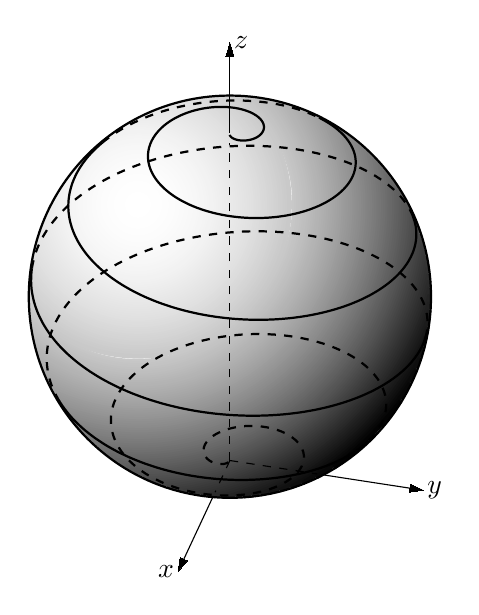
\begin{tikzpicture}[scale=2.54]
% dpic version 2019.06.20 option -g for TikZ and PGF 1.01
\ifx\dpiclw\undefined\newdimen\dpiclw\fi
\global\def\dpicdraw{\draw[line width=\dpiclw]}
\global\def\dpicstop{;}
\dpiclw=0.8bp
\dpiclw=0.8bp
\dpicdraw[line width=1.6bp,draw={rgb,1:red,0.99995;green,0.99995;blue,0.99995}](-0.459619,1.278771) circle (0.004389in)\dpicstop
\dpicdraw[line width=1.6bp,draw={rgb,1:red,0.99982;green,0.99982;blue,0.99982}](-0.459619,1.278771) circle (0.008778in)\dpicstop
\dpicdraw[line width=1.6bp,draw={rgb,1:red,0.99959;green,0.99959;blue,0.99959}](-0.459619,1.278771) circle (0.013168in)\dpicstop
\dpicdraw[line width=1.6bp,draw={rgb,1:red,0.99927;green,0.99927;blue,0.99927}](-0.459619,1.278771) circle (0.017557in)\dpicstop
\dpicdraw[line width=1.6bp,draw={rgb,1:red,0.99886;green,0.99886;blue,0.99886}](-0.459619,1.278771) circle (0.021946in)\dpicstop
\dpicdraw[line width=1.6bp,draw={rgb,1:red,0.99836;green,0.99836;blue,0.99836}](-0.459619,1.278771) circle (0.026335in)\dpicstop
\dpicdraw[line width=1.6bp,draw={rgb,1:red,0.99776;green,0.99776;blue,0.99776}](-0.459619,1.278771) circle (0.030725in)\dpicstop
\dpicdraw[line width=1.6bp,draw={rgb,1:red,0.99708;green,0.99708;blue,0.99708}](-0.459619,1.278771) circle (0.035114in)\dpicstop
\dpicdraw[line width=1.6bp,draw={rgb,1:red,0.99630;green,0.99630;blue,0.99630}](-0.459619,1.278771) circle (0.039503in)\dpicstop
\dpicdraw[line width=1.6bp,draw={rgb,1:red,0.99543;green,0.99543;blue,0.99543}](-0.459619,1.278771) circle (0.043892in)\dpicstop
\dpicdraw[line width=1.6bp,draw={rgb,1:red,0.99448;green,0.99448;blue,0.99448}](-0.459619,1.278771) circle (0.048282in)\dpicstop
\dpicdraw[line width=1.6bp,draw={rgb,1:red,0.99343;green,0.99343;blue,0.99343}](-0.459619,1.278771) circle (0.052671in)\dpicstop
\dpicdraw[line width=1.6bp,draw={rgb,1:red,0.99228;green,0.99228;blue,0.99228}](-0.459619,1.278771) circle (0.05706in)\dpicstop
\dpicdraw[line width=1.6bp,draw={rgb,1:red,0.99105;green,0.99105;blue,0.99105}](-0.459619,1.278771) circle (0.061449in)\dpicstop
\dpicdraw[line width=1.6bp,draw={rgb,1:red,0.98973;green,0.98973;blue,0.98973}](-0.459619,1.278771) circle (0.065838in)\dpicstop
\dpicdraw[line width=1.6bp,draw={rgb,1:red,0.98831;green,0.98831;blue,0.98831}](-0.459619,1.278771) circle (0.070228in)\dpicstop
\dpicdraw[line width=1.6bp,draw={rgb,1:red,0.98681;green,0.98681;blue,0.98681}](-0.459619,1.278771) circle (0.074617in)\dpicstop
\dpicdraw[line width=1.6bp,draw={rgb,1:red,0.98521;green,0.98521;blue,0.98521}](-0.459619,1.278771) circle (0.079006in)\dpicstop
\dpicdraw[line width=1.6bp,draw={rgb,1:red,0.98352;green,0.98352;blue,0.98352}](-0.459619,1.278771) circle (0.083395in)\dpicstop
\dpicdraw[line width=1.6bp,draw={rgb,1:red,0.98174;green,0.98174;blue,0.98174}](-0.459619,1.278771) circle (0.087785in)\dpicstop
\dpicdraw[line width=1.6bp,draw={rgb,1:red,0.97987;green,0.97987;blue,0.97987}](-0.459619,1.278771) circle (0.092174in)\dpicstop
\dpicdraw[line width=1.6bp,draw={rgb,1:red,0.97790;green,0.97790;blue,0.97790}](-0.459619,1.278771) circle (0.096563in)\dpicstop
\dpicdraw[line width=1.6bp,draw={rgb,1:red,0.97585;green,0.97585;blue,0.97585}](-0.459619,1.278771) circle (0.100952in)\dpicstop
\dpicdraw[line width=1.6bp,draw={rgb,1:red,0.97370;green,0.97370;blue,0.97370}](-0.459619,1.278771) circle (0.105342in)\dpicstop
\dpicdraw[line width=1.6bp,draw={rgb,1:red,0.97147;green,0.97147;blue,0.97147}](-0.459619,1.278771) circle (0.109731in)\dpicstop
\dpicdraw[line width=1.6bp,draw={rgb,1:red,0.96914;green,0.96914;blue,0.96914}](-0.459619,1.278771) circle (0.11412in)\dpicstop
\dpicdraw[line width=1.6bp,draw={rgb,1:red,0.96672;green,0.96672;blue,0.96672}](-0.459619,1.278771) circle (0.118509in)\dpicstop
\dpicdraw[line width=1.6bp,draw={rgb,1:red,0.96421;green,0.96421;blue,0.96421}](-0.459619,1.278771) circle (0.122898in)\dpicstop
\dpicdraw[line width=1.6bp,draw={rgb,1:red,0.96161;green,0.96161;blue,0.96161}](-0.459619,1.278771) circle (0.127288in)\dpicstop
\dpicdraw[line width=1.6bp,draw={rgb,1:red,0.95891;green,0.95891;blue,0.95891}](-0.459619,1.278771) circle (0.131677in)\dpicstop
\dpicdraw[line width=1.6bp,draw={rgb,1:red,0.95613;green,0.95613;blue,0.95613}](-0.459619,1.278771) circle (0.136066in)\dpicstop
\dpicdraw[line width=1.6bp,draw={rgb,1:red,0.95325;green,0.95325;blue,0.95325}](-0.643957,1.584214)
 ..controls (-0.283293,1.801877) and (0.090518,1.324378)
 ..(-0.207354,1.026506)
 ..controls (-0.505226,0.728634) and (-0.982725,1.102445)
 ..(-0.765062,1.463109)\dpicstop
\dpicdraw[line width=1.6bp,draw={rgb,1:red,0.95028;green,0.95028;blue,0.95028}](-0.600923,1.618459)
 ..controls (-0.228938,1.773197) and (0.085412,1.303506)
 ..(-0.199471,1.018623)
 ..controls (-0.484354,0.73374) and (-0.954045,1.04809)
 ..(-0.799307,1.420075)\dpicstop
\dpicdraw[line width=1.6bp,draw={rgb,1:red,0.94722;green,0.94722;blue,0.94722}](-0.568459,1.641864)
 ..controls (-0.191286,1.754924) and (0.086838,1.289166)
 ..(-0.191588,1.01074)
 ..controls (-0.470014,0.732314) and (-0.935772,1.010438)
 ..(-0.822712,1.387611)\dpicstop
\dpicdraw[line width=1.6bp,draw={rgb,1:red,0.94407;green,0.94407;blue,0.94407}](-0.540491,1.660502)
 ..controls (-0.160556,1.740993) and (0.090914,1.277475)
 ..(-0.183704,1.002856)
 ..controls (-0.458322,0.728238) and (-0.921841,0.979708)
 ..(-0.841349,1.359644)\dpicstop
\dpicdraw[line width=1.6bp,draw={rgb,1:red,0.94083;green,0.94083;blue,0.94083}](-0.515127,1.676266)
 ..controls (-0.133764,1.729521) and (0.09646,1.267254)
 ..(-0.175821,0.994973)
 ..controls (-0.448102,0.722692) and (-0.910369,0.952916)
 ..(-0.857114,1.334279)\dpicstop
\dpicdraw[line width=1.6bp,draw={rgb,1:red,0.93750;green,0.93750;blue,0.93750}](-0.491484,1.690039)
 ..controls (-0.109548,1.71963) and (0.102941,1.257969)
 ..(-0.167938,0.98709)
 ..controls (-0.438816,0.716211) and (-0.900478,0.9287)
 ..(-0.870887,1.310636)\dpicstop
\dpicdraw[line width=1.6bp,draw={rgb,1:red,0.93408;green,0.93408;blue,0.93408}](-0.469067,1.702315)
 ..controls (-0.087159,1.710833) and (0.110062,1.249324)
 ..(-0.160055,0.979207)
 ..controls (-0.430172,0.70909) and (-0.891681,0.906311)
 ..(-0.883163,1.288219)\dpicstop
\dpicdraw[line width=1.6bp,draw={rgb,1:red,0.93056;green,0.93056;blue,0.93056}](-0.447568,1.713402)
 ..controls (-0.066136,1.702826) and (0.117645,1.24114)
 ..(-0.152171,0.971323)
 ..controls (-0.421988,0.701507) and (-0.883674,0.885289)
 ..(-0.89425,1.266721)\dpicstop
\dpicdraw[line width=1.6bp,draw={rgb,1:red,0.92695;green,0.92695;blue,0.92695}](-0.426782,1.723507)
 ..controls (-0.046179,1.695404) and (0.125572,1.2333)
 ..(-0.144288,0.96344)
 ..controls (-0.414148,0.69358) and (-0.876252,0.865331)
 ..(-0.904355,1.245934)\dpicstop
\dpicdraw[line width=1.6bp,draw={rgb,1:red,0.92326;green,0.92326;blue,0.92326}](-0.40656,1.732776)
 ..controls (-0.027074,1.688426) and (0.133759,1.22572)
 ..(-0.136405,0.955557)
 ..controls (-0.406568,0.685393) and (-0.869274,0.846226)
 ..(-0.913624,1.225712)\dpicstop
\dpicdraw[line width=1.6bp,draw={rgb,1:red,0.91947;green,0.91947;blue,0.91947}](-0.386796,1.741317)
 ..controls (-0.00867,1.681785) and (0.142148,1.218343)
 ..(-0.128521,0.947673)
 ..controls (-0.399191,0.677004) and (-0.862633,0.827822)
 ..(-0.922165,1.205948)\dpicstop
\dpicdraw[line width=1.6bp,draw={rgb,1:red,0.91559;green,0.91559;blue,0.91559}](-0.367409,1.749211)
 ..controls (0.009148,1.675403) and (0.150695,1.211123)
 ..(-0.120638,0.93979)
 ..controls (-0.391971,0.668457) and (-0.856251,0.810004)
 ..(-0.930059,1.186561)\dpicstop
\dpicdraw[line width=1.6bp,draw={rgb,1:red,0.91161;green,0.91161;blue,0.91161}](-0.348335,1.756522)
 ..controls (0.026467,1.669218) and (0.159365,1.204027)
 ..(-0.112755,0.931907)
 ..controls (-0.384875,0.659787) and (-0.850066,0.792685)
 ..(-0.93737,1.167487)\dpicstop
\dpicdraw[line width=1.6bp,draw={rgb,1:red,0.90755;green,0.90755;blue,0.90755}](-0.329524,1.763299)
 ..controls (0.043355,1.663181) and (0.168132,1.197028)
 ..(-0.104872,0.924024)
 ..controls (-0.377876,0.65102) and (-0.844029,0.775797)
 ..(-0.944147,1.148676)\dpicstop
\dpicdraw[line width=1.6bp,draw={rgb,1:red,0.90340;green,0.90340;blue,0.90340}](-0.310936,1.769583)
 ..controls (0.059867,1.657254) and (0.176976,1.190105)
 ..(-0.096988,0.91614)
 ..controls (-0.370953,0.642176) and (-0.838102,0.759285)
 ..(-0.950431,1.130088)\dpicstop
\dpicdraw[line width=1.6bp,draw={rgb,1:red,0.89915;green,0.89915;blue,0.89915}](-0.292538,1.775406)
 ..controls (0.076047,1.651404) and (0.185879,1.183241)
 ..(-0.089105,0.908257)
 ..controls (-0.364089,0.633273) and (-0.832252,0.743105)
 ..(-0.956254,1.11169)\dpicstop
\dpicdraw[line width=1.6bp,draw={rgb,1:red,0.89481;green,0.89481;blue,0.89481}](-0.274304,1.780795)
 ..controls (0.091931,1.645604) and (0.194826,1.176422)
 ..(-0.081222,0.900374)
 ..controls (-0.35727,0.624326) and (-0.826452,0.727221)
 ..(-0.961643,1.093456)\dpicstop
\dpicdraw[line width=1.6bp,draw={rgb,1:red,0.89039;green,0.89039;blue,0.89039}](-0.25621,1.785773)
 ..controls (0.107549,1.639833) and (0.203807,1.169636)
 ..(-0.073338,0.89249)
 ..controls (-0.350484,0.615345) and (-0.820681,0.711603)
 ..(-0.966621,1.075362)\dpicstop
\dpicdraw[line width=1.6bp,draw={rgb,1:red,0.88587;green,0.88587;blue,0.88587}](-0.238239,1.790359)
 ..controls (0.122924,1.634071) and (0.212811,1.162874)
 ..(-0.065455,0.884607)
 ..controls (-0.343722,0.606341) and (-0.814919,0.696228)
 ..(-0.971207,1.057391)\dpicstop
\dpicdraw[line width=1.6bp,draw={rgb,1:red,0.88125;green,0.88125;blue,0.88125}](-0.220373,1.794568)
 ..controls (0.138079,1.628304) and (0.221831,1.156127)
 ..(-0.057572,0.876724)
 ..controls (-0.336975,0.597321) and (-0.809152,0.681073)
 ..(-0.975416,1.039525)\dpicstop
\dpicdraw[line width=1.6bp,draw={rgb,1:red,0.87655;green,0.87655;blue,0.87655}](-0.202601,1.798414)
 ..controls (0.153031,1.622516) and (0.230859,1.149388)
 ..(-0.049689,0.868841)
 ..controls (-0.330236,0.588293) and (-0.803364,0.666121)
 ..(-0.979261,1.021753)\dpicstop
\dpicdraw[line width=1.6bp,draw={rgb,1:red,0.87176;green,0.87176;blue,0.87176}](-0.184909,1.801908)
 ..controls (0.167794,1.616695) and (0.239889,1.142652)
 ..(-0.041805,0.860957)
 ..controls (-0.323499,0.579263) and (-0.797543,0.651358)
 ..(-0.982756,1.004061)\dpicstop
\dpicdraw[line width=1.6bp,draw={rgb,1:red,0.86687;green,0.86687;blue,0.86687}](-0.167289,1.80506)
 ..controls (0.182382,1.610833) and (0.248916,1.135912)
 ..(-0.033922,0.853074)
 ..controls (-0.31676,0.570236) and (-0.791681,0.63677)
 ..(-0.985908,0.986441)\dpicstop
\dpicdraw[line width=1.6bp,draw={rgb,1:red,0.86190;green,0.86190;blue,0.86190}](-0.149732,1.807879)
 ..controls (0.196806,1.604918) and (0.257935,1.129164)
 ..(-0.026039,0.845191)
 ..controls (-0.310012,0.561217) and (-0.785766,0.622346)
 ..(-0.988727,0.968884)\dpicstop
\dpicdraw[line width=1.6bp,draw={rgb,1:red,0.85683;green,0.85683;blue,0.85683}](-0.132231,1.810371)
 ..controls (0.211076,1.598944) and (0.266942,1.122405)
 ..(-0.018155,0.837307)
 ..controls (-0.303253,0.55221) and (-0.779792,0.608076)
 ..(-0.991219,0.951383)\dpicstop
\dpicdraw[line width=1.6bp,draw={rgb,1:red,0.85167;green,0.85167;blue,0.85167}](-0.11478,1.812543)
 ..controls (0.225199,1.592902) and (0.275934,1.11563)
 ..(-0.010272,0.829424)
 ..controls (-0.296478,0.543218) and (-0.77375,0.593953)
 ..(-0.993391,0.933932)\dpicstop
\dpicdraw[line width=1.6bp,draw={rgb,1:red,0.84642;green,0.84642;blue,0.84642}](-0.097374,1.8144)
 ..controls (0.239183,1.586787) and (0.284907,1.108837)
 ..(-0.002389,0.821541)
 ..controls (-0.289685,0.534245) and (-0.767635,0.57997)
 ..(-0.995248,0.916526)\dpicstop
\dpicdraw[line width=1.6bp,draw={rgb,1:red,0.84108;green,0.84108;blue,0.84108}](-0.080008,1.815946)
 ..controls (0.253033,1.580592) and (0.293859,1.102022)
 ..(0.005494,0.813658)
 ..controls (-0.28287,0.525293) and (-0.76144,0.566119)
 ..(-0.996794,0.89916)\dpicstop
\dpicdraw[line width=1.6bp,draw={rgb,1:red,0.83565;green,0.83565;blue,0.83565}](-0.062678,1.817186)
 ..controls (0.266757,1.574313) and (0.302786,1.095183)
 ..(0.013378,0.805774)
 ..controls (-0.276031,0.516366) and (-0.755161,0.552395)
 ..(-0.998034,0.88183)\dpicstop
\dpicdraw[line width=1.6bp,draw={rgb,1:red,0.83012;green,0.83012;blue,0.83012}](-0.045381,1.818122)
 ..controls (0.280358,1.567944) and (0.311687,1.088318)
 ..(0.021261,0.797891)
 ..controls (-0.269165,0.507465) and (-0.748792,0.538794)
 ..(-0.99897,0.864533)\dpicstop
\dpicdraw[line width=1.6bp,draw={rgb,1:red,0.82451;green,0.82451;blue,0.82451}](-0.028115,1.818757)
 ..controls (0.29384,1.561481) and (0.32056,1.081423)
 ..(0.029144,0.790008)
 ..controls (-0.262271,0.498592) and (-0.742329,0.525312)
 ..(-0.999605,0.847267)\dpicstop
\dpicdraw[line width=1.6bp,draw={rgb,1:red,0.81880;green,0.81880;blue,0.81880}](-0.010878,1.819093)
 ..controls (0.307207,1.55492) and (0.329402,1.074499)
 ..(0.037028,0.782124)
 ..controls (-0.255347,0.48975) and (-0.735768,0.511945)
 ..(-0.999941,0.83003)\dpicstop
\dpicdraw[line width=1.6bp,draw={rgb,1:red,0.81300;green,0.81300;blue,0.81300}](0.006333,1.819132)
 ..controls (0.320463,1.548258) and (0.338211,1.067541)
 ..(0.044911,0.774241)
 ..controls (-0.248389,0.480941) and (-0.729106,0.498689)
 ..(-0.99998,0.812819)\dpicstop
\dpicdraw[line width=1.6bp,draw={rgb,1:red,0.80711;green,0.80711;blue,0.80711}](0.023519,1.818875)
 ..controls (0.333609,1.541491) and (0.346986,1.06055)
 ..(0.052794,0.766358)
 ..controls (-0.241398,0.472166) and (-0.722339,0.485543)
 ..(-0.999723,0.795633)\dpicstop
\dpicdraw[line width=1.6bp,draw={rgb,1:red,0.80113;green,0.80113;blue,0.80113}](0.040681,1.818324)
 ..controls (0.346649,1.534615) and (0.355726,1.053523)
 ..(0.060677,0.758475)
 ..controls (-0.234371,0.463426) and (-0.715463,0.472503)
 ..(-0.999172,0.778471)\dpicstop
\dpicdraw[line width=1.6bp,draw={rgb,1:red,0.79506;green,0.79506;blue,0.79506}](0.057819,1.817479)
 ..controls (0.359584,1.527628) and (0.364429,1.046459)
 ..(0.068561,0.750591)
 ..controls (-0.227307,0.454723) and (-0.708476,0.459568)
 ..(-0.998327,0.761333)\dpicstop
\dpicdraw[line width=1.6bp,draw={rgb,1:red,0.78890;green,0.78890;blue,0.78890}](0.074934,1.816341)
 ..controls (0.372416,1.520527) and (0.373093,1.039357)
 ..(0.076444,0.742708)
 ..controls (-0.220205,0.446059) and (-0.701375,0.446736)
 ..(-0.997188,0.744218)\dpicstop
\dpicdraw[line width=1.6bp,draw={rgb,1:red,0.78264;green,0.78264;blue,0.78264}](0.092026,1.814909)
 ..controls (0.796757,1.089793) and (-0.270641,0.022395)
 ..(-0.995757,0.727126)\dpicstop
\dpicdraw[line width=1.6bp,draw={rgb,1:red,0.77630;green,0.77630;blue,0.77630}](0.109095,1.813183)
 ..controls (0.799831,1.07811) and (-0.258958,0.019321)
 ..(-0.994031,0.710057)\dpicstop
\dpicdraw[line width=1.6bp,draw={rgb,1:red,0.76986;green,0.76986;blue,0.76986}](0.126141,1.811164)
 ..controls (0.802926,1.066538) and (-0.247386,0.016226)
 ..(-0.992012,0.693011)\dpicstop
\dpicdraw[line width=1.6bp,draw={rgb,1:red,0.76333;green,0.76333;blue,0.76333}](0.143163,1.808851)
 ..controls (0.806032,1.055067) and (-0.235915,0.01312)
 ..(-0.989699,0.675989)\dpicstop
\dpicdraw[line width=1.6bp,draw={rgb,1:red,0.75671;green,0.75671;blue,0.75671}](0.160161,1.806243)
 ..controls (0.809141,1.043689) and (-0.224537,0.010011)
 ..(-0.987091,0.658991)\dpicstop
\dpicdraw[line width=1.6bp,draw={rgb,1:red,0.75000;green,0.75000;blue,0.75000}](0.177133,1.803339)
 ..controls (0.812247,1.032398) and (-0.213246,0.006905)
 ..(-0.984187,0.642019)\dpicstop
\dpicdraw[line width=1.6bp,draw={rgb,1:red,0.74320;green,0.74320;blue,0.74320}](0.194079,1.800138)
 ..controls (0.815342,1.021187) and (-0.202035,0.00381)
 ..(-0.980986,0.625073)\dpicstop
\dpicdraw[line width=1.6bp,draw={rgb,1:red,0.73630;green,0.73630;blue,0.73630}](0.210997,1.796639)
 ..controls (0.818422,1.01005) and (-0.190898,0.000731)
 ..(-0.977487,0.608155)\dpicstop
\dpicdraw[line width=1.6bp,draw={rgb,1:red,0.72932;green,0.72932;blue,0.72932}](0.227885,1.79284)
 ..controls (0.821479,0.99898) and (-0.179828,-0.002327)
 ..(-0.973688,0.591267)\dpicstop
\dpicdraw[line width=1.6bp,draw={rgb,1:red,0.72224;green,0.72224;blue,0.72224}](0.244743,1.78874)
 ..controls (0.824509,0.987974) and (-0.168822,-0.005357)
 ..(-0.969588,0.574409)\dpicstop
\dpicdraw[line width=1.6bp,draw={rgb,1:red,0.71507;green,0.71507;blue,0.71507}](0.261569,1.784337)
 ..controls (0.827507,0.977027) and (-0.157875,-0.008355)
 ..(-0.965185,0.557583)\dpicstop
\dpicdraw[line width=1.6bp,draw={rgb,1:red,0.70782;green,0.70782;blue,0.70782}](0.278359,1.779629)
 ..controls (0.830469,0.966133) and (-0.146981,-0.011317)
 ..(-0.960477,0.540793)\dpicstop
\dpicdraw[line width=1.6bp,draw={rgb,1:red,0.70047;green,0.70047;blue,0.70047}](0.295114,1.774614)
 ..controls (0.833392,0.95529) and (-0.136138,-0.014239)
 ..(-0.955462,0.524038)\dpicstop
\dpicdraw[line width=1.6bp,draw={rgb,1:red,0.69302;green,0.69302;blue,0.69302}](0.311829,1.76929)
 ..controls (0.83627,0.944492) and (-0.12534,-0.017118)
 ..(-0.950138,0.507323)\dpicstop
\dpicdraw[line width=1.6bp,draw={rgb,1:red,0.68549;green,0.68549;blue,0.68549}](0.328504,1.763655)
 ..controls (0.8391,0.933737) and (-0.114585,-0.019948)
 ..(-0.944503,0.490648)\dpicstop
\dpicdraw[line width=1.6bp,draw={rgb,1:red,0.67787;green,0.67787;blue,0.67787}](0.345135,1.757705)
 ..controls (0.84188,0.923022) and (-0.10387,-0.022728)
 ..(-0.938553,0.474017)\dpicstop
\dpicdraw[line width=1.6bp,draw={rgb,1:red,0.67015;green,0.67015;blue,0.67015}](0.36172,1.751439)
 ..controls (0.844606,0.912343) and (-0.093191,-0.025454)
 ..(-0.932287,0.457432)\dpicstop
\dpicdraw[line width=1.6bp,draw={rgb,1:red,0.66234;green,0.66234;blue,0.66234}](0.378255,1.744853)
 ..controls (0.847275,0.901697) and (-0.082545,-0.028123)
 ..(-0.925701,0.440897)\dpicstop
\dpicdraw[line width=1.6bp,draw={rgb,1:red,0.65445;green,0.65445;blue,0.65445}](0.394739,1.737945)
 ..controls (0.849885,0.891082) and (-0.07193,-0.030733)
 ..(-0.918793,0.424413)\dpicstop
\dpicdraw[line width=1.6bp,draw={rgb,1:red,0.64646;green,0.64646;blue,0.64646}](0.411168,1.730712)
 ..controls (0.852432,0.880494) and (-0.061342,-0.03328)
 ..(-0.91156,0.407984)\dpicstop
\dpicdraw[line width=1.6bp,draw={rgb,1:red,0.63838;green,0.63838;blue,0.63838}](0.427538,1.723149)
 ..controls (0.854915,0.869933) and (-0.050781,-0.035763)
 ..(-0.903997,0.391614)\dpicstop
\dpicdraw[line width=1.6bp,draw={rgb,1:red,0.63020;green,0.63020;blue,0.63020}](0.443846,1.715255)
 ..controls (0.857331,0.859394) and (-0.040242,-0.038179)
 ..(-0.896103,0.375306)\dpicstop
\dpicdraw[line width=1.6bp,draw={rgb,1:red,0.62194;green,0.62194;blue,0.62194}](0.460089,1.707025)
 ..controls (0.859678,0.848876) and (-0.029724,-0.040525)
 ..(-0.887873,0.359063)\dpicstop
\dpicdraw[line width=1.6bp,draw={rgb,1:red,0.61359;green,0.61359;blue,0.61359}](0.476263,1.698455)
 ..controls (0.861953,0.838377) and (-0.019225,-0.042801)
 ..(-0.879303,0.342889)\dpicstop
\dpicdraw[line width=1.6bp,draw={rgb,1:red,0.60514;green,0.60514;blue,0.60514}](0.492364,1.689541)
 ..controls (0.864154,0.827895) and (-0.008743,-0.045002)
 ..(-0.870389,0.326788)\dpicstop
\dpicdraw[line width=1.6bp,draw={rgb,1:red,0.59660;green,0.59660;blue,0.59660}](0.508388,1.68028)
 ..controls (0.866281,0.817428) and (0.001724,-0.047129)
 ..(-0.861128,0.310764)\dpicstop
\dpicdraw[line width=1.6bp,draw={rgb,1:red,0.58797;green,0.58797;blue,0.58797}](0.52433,1.670667)
 ..controls (0.86833,0.806973) and (0.012179,-0.049178)
 ..(-0.851515,0.294822)\dpicstop
\dpicdraw[line width=1.6bp,draw={rgb,1:red,0.57925;green,0.57925;blue,0.57925}](0.540186,1.660698)
 ..controls (0.870299,0.796529) and (0.022623,-0.051147)
 ..(-0.841546,0.278966)\dpicstop
\dpicdraw[line width=1.6bp,draw={rgb,1:red,0.57044;green,0.57044;blue,0.57044}](0.555951,1.650367)
 ..controls (0.872187,0.786094) and (0.033059,-0.053035)
 ..(-0.831215,0.263201)\dpicstop
\dpicdraw[line width=1.6bp,draw={rgb,1:red,0.56154;green,0.56154;blue,0.56154}](0.571621,1.63967)
 ..controls (0.873993,0.775665) and (0.043487,-0.054841)
 ..(-0.820518,0.247531)\dpicstop
\dpicdraw[line width=1.6bp,draw={rgb,1:red,0.55255;green,0.55255;blue,0.55255}](0.587189,1.628602)
 ..controls (0.875713,0.765243) and (0.053909,-0.056561)
 ..(-0.80945,0.231963)\dpicstop
\dpicdraw[line width=1.6bp,draw={rgb,1:red,0.54346;green,0.54346;blue,0.54346}](0.602651,1.617157)
 ..controls (0.877347,0.754823) and (0.064329,-0.058195)
 ..(-0.798005,0.216501)\dpicstop
\dpicdraw[line width=1.6bp,draw={rgb,1:red,0.53429;green,0.53429;blue,0.53429}](0.618001,1.605329)
 ..controls (0.878892,0.744406) and (0.074746,-0.05974)
 ..(-0.786177,0.201151)\dpicstop
\dpicdraw[line width=1.6bp,draw={rgb,1:red,0.52502;green,0.52502;blue,0.52502}](0.633233,1.593113)
 ..controls (0.880347,0.733988) and (0.085164,-0.061195)
 ..(-0.773961,0.185919)\dpicstop
\dpicdraw[line width=1.6bp,draw={rgb,1:red,0.51566;green,0.51566;blue,0.51566}](0.648341,1.580502)
 ..controls (0.88171,0.723568) and (0.095584,-0.062558)
 ..(-0.76135,0.170811)\dpicstop
\dpicdraw[line width=1.6bp,draw={rgb,1:red,0.50621;green,0.50621;blue,0.50621}](0.663318,1.56749)
 ..controls (0.882979,0.713145) and (0.106007,-0.063826)
 ..(-0.748338,0.155834)\dpicstop
\dpicdraw[line width=1.6bp,draw={rgb,1:red,0.49667;green,0.49667;blue,0.49667}](0.678157,1.554069)
 ..controls (0.884152,0.702715) and (0.116437,-0.065)
 ..(-0.734917,0.140995)\dpicstop
\dpicdraw[line width=1.6bp,draw={rgb,1:red,0.48703;green,0.48703;blue,0.48703}](0.69285,1.540233)
 ..controls (0.885227,0.692278) and (0.126874,-0.066075)
 ..(-0.721081,0.126302)\dpicstop
\dpicdraw[line width=1.6bp,draw={rgb,1:red,0.47731;green,0.47731;blue,0.47731}](0.707391,1.525974)
 ..controls (0.886202,0.681832) and (0.13732,-0.06705)
 ..(-0.706822,0.111761)\dpicstop
\dpicdraw[line width=1.6bp,draw={rgb,1:red,0.46749;green,0.46749;blue,0.46749}](0.721771,1.511284)
 ..controls (0.887076,0.671374) and (0.147778,-0.067924)
 ..(-0.692132,0.097381)\dpicstop
\dpicdraw[line width=1.6bp,draw={rgb,1:red,0.45759;green,0.45759;blue,0.45759}](0.735982,1.496153)
 ..controls (0.887846,0.660902) and (0.15825,-0.068694)
 ..(-0.677001,0.08317)\dpicstop
\dpicdraw[line width=1.6bp,draw={rgb,1:red,0.44759;green,0.44759;blue,0.44759}](0.750014,1.480574)
 ..controls (0.888509,0.650414) and (0.168738,-0.069357)
 ..(-0.661422,0.069138)\dpicstop
\dpicdraw[line width=1.6bp,draw={rgb,1:red,0.43750;green,0.43750;blue,0.43750}](0.763858,1.464536)
 ..controls (0.889064,0.639907) and (0.179245,-0.069912)
 ..(-0.645384,0.055294)\dpicstop
\dpicdraw[line width=1.6bp,draw={rgb,1:red,0.42732;green,0.42732;blue,0.42732}](0.777504,1.44803)
 ..controls (0.889509,0.62938) and (0.189772,-0.070357)
 ..(-0.628878,0.041648)\dpicstop
\dpicdraw[line width=1.6bp,draw={rgb,1:red,0.41705;green,0.41705;blue,0.41705}](0.790941,1.431044)
 ..controls (0.889839,0.61883) and (0.200322,-0.070687)
 ..(-0.611892,0.028211)\dpicstop
\dpicdraw[line width=1.6bp,draw={rgb,1:red,0.40668;green,0.40668;blue,0.40668}](0.804158,1.413567)
 ..controls (0.890054,0.608253) and (0.210899,-0.070902)
 ..(-0.594415,0.014994)\dpicstop
\dpicdraw[line width=1.6bp,draw={rgb,1:red,0.39623;green,0.39623;blue,0.39623}](0.817142,1.395588)
 ..controls (0.890149,0.597648) and (0.221504,-0.070997)
 ..(-0.576436,0.00201)\dpicstop
\dpicdraw[line width=1.6bp,draw={rgb,1:red,0.38568;green,0.38568;blue,0.38568}](0.829881,1.377093)
 ..controls (0.890123,0.58701) and (0.232142,-0.070971)
 ..(-0.557941,-0.010729)\dpicstop
\dpicdraw[line width=1.6bp,draw={rgb,1:red,0.37505;green,0.37505;blue,0.37505}](0.84236,1.358067)
 ..controls (0.889971,0.576338) and (0.242814,-0.070818)
 ..(-0.538915,-0.023208)\dpicstop
\dpicdraw[line width=1.6bp,draw={rgb,1:red,0.36432;green,0.36432;blue,0.36432}](0.854565,1.338497)
 ..controls (0.889689,0.565626) and (0.253526,-0.070537)
 ..(-0.519345,-0.035413)\dpicstop
\dpicdraw[line width=1.6bp,draw={rgb,1:red,0.35350;green,0.35350;blue,0.35350}](0.866479,1.318366)
 ..controls (0.889275,0.554871) and (0.264281,-0.070123)
 ..(-0.499214,-0.047327)\dpicstop
\dpicdraw[line width=1.6bp,draw={rgb,1:red,0.34259;green,0.34259;blue,0.34259}](0.878085,1.297656)
 ..controls (0.888724,0.54407) and (0.275082,-0.069572)
 ..(-0.478504,-0.058933)\dpicstop
\dpicdraw[line width=1.6bp,draw={rgb,1:red,0.33158;green,0.33158;blue,0.33158}](0.889365,1.27635)
 ..controls (0.888031,0.533217) and (0.285935,-0.068879)
 ..(-0.457198,-0.070213)\dpicstop
\dpicdraw[line width=1.6bp,draw={rgb,1:red,0.32049;green,0.32049;blue,0.32049}](0.900298,1.254426)
 ..controls (0.887192,0.522308) and (0.296844,-0.06804)
 ..(-0.435274,-0.081146)\dpicstop
\dpicdraw[line width=1.6bp,draw={rgb,1:red,0.30930;green,0.30930;blue,0.30930}](0.910862,1.231863)
 ..controls (0.8862,0.511337) and (0.307816,-0.067048)
 ..(-0.412711,-0.09171)\dpicstop
\dpicdraw[line width=1.6bp,draw={rgb,1:red,0.29803;green,0.29803;blue,0.29803}](0.921033,1.208637)
 ..controls (0.885051,0.500297) and (0.318855,-0.065899)
 ..(-0.389485,-0.101881)\dpicstop
\dpicdraw[line width=1.6bp,draw={rgb,1:red,0.28666;green,0.28666;blue,0.28666}](0.930784,1.184721)
 ..controls (0.883736,0.489184) and (0.329968,-0.064584)
 ..(-0.365569,-0.111632)\dpicstop
\dpicdraw[line width=1.6bp,draw={rgb,1:red,0.27520;green,0.27520;blue,0.27520}](0.940087,1.160085)
 ..controls (0.88225,0.477988) and (0.341164,-0.063098)
 ..(-0.340933,-0.120935)\dpicstop
\dpicdraw[line width=1.6bp,draw={rgb,1:red,0.26365;green,0.26365;blue,0.26365}](0.94891,1.134699)
 ..controls (0.880583,0.466702) and (0.35245,-0.061431)
 ..(-0.315547,-0.129758)\dpicstop
\dpicdraw[line width=1.6bp,draw={rgb,1:red,0.25201;green,0.25201;blue,0.25201}](0.957216,1.108526)
 ..controls (0.878727,0.455317) and (0.363835,-0.059575)
 ..(-0.289374,-0.138064)\dpicstop
\dpicdraw[line width=1.6bp,draw={rgb,1:red,0.24028;green,0.24028;blue,0.24028}](0.964966,1.081527)
 ..controls (0.876671,0.443822) and (0.37533,-0.057519)
 ..(-0.262375,-0.145814)\dpicstop
\dpicdraw[line width=1.6bp,draw={rgb,1:red,0.22845;green,0.22845;blue,0.22845}](0.972115,1.053656)
 ..controls (0.874403,0.432205) and (0.386947,-0.055251)
 ..(-0.234504,-0.152963)\dpicstop
\dpicdraw[line width=1.6bp,draw={rgb,1:red,0.21654;green,0.21654;blue,0.21654}](0.978613,1.024863)
 ..controls (0.871909,0.420452) and (0.3987,-0.052757)
 ..(-0.205711,-0.159461)\dpicstop
\dpicdraw[line width=1.6bp,draw={rgb,1:red,0.20453;green,0.20453;blue,0.20453}](0.984401,0.995091)
 ..controls (0.869174,0.408549) and (0.410603,-0.050022)
 ..(-0.175939,-0.165249)\dpicstop
\dpicdraw[line width=1.6bp,draw={rgb,1:red,0.19243;green,0.19243;blue,0.19243}](0.989414,0.964272)
 ..controls (0.866179,0.396476) and (0.422676,-0.047027)
 ..(-0.14512,-0.170262)\dpicstop
\dpicdraw[line width=1.6bp,draw={rgb,1:red,0.18024;green,0.18024;blue,0.18024}](0.993575,0.932331)
 ..controls (0.862903,0.384212) and (0.43494,-0.043751)
 ..(-0.113179,-0.174423)\dpicstop
\dpicdraw[line width=1.6bp,draw={rgb,1:red,0.16796;green,0.16796;blue,0.16796}](0.996793,0.899177)
 ..controls (0.859321,0.371732) and (0.44742,-0.040169)
 ..(-0.080025,-0.177641)\dpicstop
\dpicdraw[line width=1.6bp,draw={rgb,1:red,0.15559;green,0.15559;blue,0.15559}](0.998962,0.864704)
 ..controls (0.855402,0.359005) and (0.460147,-0.03625)
 ..(-0.045552,-0.17981)\dpicstop
\dpicdraw[line width=1.6bp,draw={rgb,1:red,0.14312;green,0.14312;blue,0.14312}](0.999954,0.828783)
 ..controls (0.851109,0.345994) and (0.473158,-0.031957)
 ..(-0.009631,-0.180802)\dpicstop
\dpicdraw[line width=1.6bp,draw={rgb,1:red,0.13057;green,0.13057;blue,0.13057}](0.999611,0.791256)
 ..controls (0.846396,0.332653) and (0.486499,-0.027244)
 ..(0.027896,-0.180459)\dpicstop
\dpicdraw[line width=1.6bp,draw={rgb,1:red,0.11792;green,0.11792;blue,0.11792}](0.997738,0.75193)
 ..controls (0.841204,0.318924) and (0.500228,-0.022052)
 ..(0.067222,-0.178586)\dpicstop
\dpicdraw[line width=1.6bp,draw={rgb,1:red,0.10519;green,0.10519;blue,0.10519}](0.994086,0.710553)
 ..controls (0.83546,0.304732) and (0.51442,-0.016308)
 ..(0.108599,-0.174934)\dpicstop
\dpicdraw[line width=1.6bp,draw={rgb,1:red,0.09236;green,0.09236;blue,0.09236}](0.988326,0.666799)
 ..controls (0.829063,0.289978) and (0.529174,-0.009911)
 ..(0.152353,-0.169174)\dpicstop
\dpicdraw[line width=1.6bp,draw={rgb,1:red,0.07944;green,0.07944;blue,0.07944}](0.980014,0.620221)
 ..controls (0.821877,0.274525) and (0.544627,-0.002725)
 ..(0.198931,-0.160862)\dpicstop
\dpicdraw[line width=1.6bp,draw={rgb,1:red,0.06643;green,0.06643;blue,0.06643}](0.968512,0.570184)
 ..controls (0.813704,0.258175) and (0.560977,0.005448)
 ..(0.248968,-0.14936)\dpicstop
\dpicdraw[line width=1.6bp,draw={rgb,1:red,0.05332;green,0.05332;blue,0.05332}](0.952853,0.515719)
 ..controls (0.804239,0.240624) and (0.578528,0.014913)
 ..(0.303433,-0.133701)\dpicstop
\dpicdraw[line width=1.6bp,draw={rgb,1:red,0.04013;green,0.04013;blue,0.04013}](0.931423,0.455213)
 ..controls (0.79297,0.221358) and (0.597794,0.026182)
 ..(0.363939,-0.112271)\dpicstop
\dpicdraw[line width=1.6bp,draw={rgb,1:red,0.02684;green,0.02684;blue,0.02684}](0.901102,0.385546)
 ..controls (0.778892,0.199373) and (0.619779,0.04026)
 ..(0.433606,-0.08195)\dpicstop
\dpicdraw[line width=1.6bp,draw={rgb,1:red,0.01347;green,0.01347;blue,0.01347}](0.853917,0.298744)
 ..controls (0.75941,0.172075) and (0.647077,0.059742)
 ..(0.520409,-0.034765)\dpicstop
\dpicdraw[line width=1.6bp,draw={rgb,1:red,0.00000;green,0.00000;blue,0.00000}](0.707107,0.112045)
 ..controls (0.707107,0.112045) and (0.707107,0.112045)
 ..(0.707107,0.112045)\dpicstop
\dpicdraw (0,0.819152) circle (0.395888in)\dpicstop
\dpicdraw[dashed](-0.007923,-0.008794)
 ..controls (-0.008878,-0.009374) and (-0.01061,-0.01038)
 ..(-0.011789,-0.011039)
 ..controls (-0.012967,-0.011699) and (-0.015095,-0.012699)
 ..(-0.016536,-0.013271)
 ..controls (-0.017978,-0.013843) and (-0.020724,-0.014729)
 ..(-0.022663,-0.015247)
 ..controls (-0.024602,-0.015765) and (-0.027919,-0.016458)
 ..(-0.030064,-0.016794)
 ..controls (-0.032209,-0.017129) and (-0.035829,-0.017514)
 ..(-0.03814,-0.017653)
 ..controls (-0.040451,-0.017791) and (-0.044308,-0.017845)
 ..(-0.046746,-0.017773)
 ..controls (-0.049183,-0.017702) and (-0.053209,-0.017406)
 ..(-0.055728,-0.017113)
 ..controls (-0.058247,-0.016821) and (-0.06237,-0.016161)
 ..(-0.064925,-0.01564)
 ..controls (-0.067481,-0.01512) and (-0.071624,-0.014086)
 ..(-0.07417,-0.013334)
 ..controls (-0.076715,-0.012581) and (-0.080802,-0.011169)
 ..(-0.083288,-0.010183)
 ..controls (-0.085774,-0.009197) and (-0.089726,-0.007407)
 ..(-0.092105,-0.006189)
 ..controls (-0.094484,-0.004972) and (-0.098223,-0.00281)
 ..(-0.100447,-0.001366)
 ..controls (-0.102671,0.000078) and (-0.106119,0.002601)
 ..(-0.10814,0.004263)
 ..controls (-0.110161,0.005925) and (-0.113242,0.008793)
 ..(-0.115015,0.010662)
 ..controls (-0.116787,0.012531) and (-0.11943,0.015723)
 ..(-0.12091,0.017784)
 ..controls (-0.12239,0.019845) and (-0.124524,0.023336)
 ..(-0.12567,0.025572)
 ..controls (-0.126817,0.027808) and (-0.128378,0.031567)
 ..(-0.129153,0.033958)
 ..controls (-0.129929,0.036349) and (-0.130858,0.040341)
 ..(-0.131227,0.042865)
 ..controls (-0.131597,0.045388) and (-0.131842,0.049575)
 ..(-0.131776,0.052206)
 ..controls (-0.131709,0.054837) and (-0.131225,0.059177)
 ..(-0.130697,0.061889)
 ..controls (-0.130169,0.0646) and (-0.128919,0.069047)
 ..(-0.127908,0.07181)
 ..controls (-0.126897,0.074573) and (-0.124852,0.07908)
 ..(-0.123344,0.081865)
 ..controls (-0.121836,0.084649) and (-0.118974,0.089165)
 ..(-0.116959,0.091939)
 ..controls (-0.114944,0.094714) and (-0.111255,0.099187)
 ..(-0.10873,0.10192)
 ..controls (-0.106204,0.104652) and (-0.101688,0.10903)
 ..(-0.098654,0.111687)
 ..controls (-0.095619,0.114344) and (-0.090284,0.118573)
 ..(-0.08675,0.121123)
 ..controls (-0.083216,0.123672) and (-0.07708,0.127699)
 ..(-0.073061,0.130108)
 ..controls (-0.069042,0.132516) and (-0.062135,0.136289)
 ..(-0.057651,0.138526)
 ..controls (-0.053167,0.140762) and (-0.045528,0.144229)
 ..(-0.040606,0.146262)
 ..controls (-0.035685,0.148294) and (-0.027361,0.151407)
 ..(-0.022036,0.153206)
 ..controls (-0.01671,0.155005) and (-0.00776,0.157716)
 ..(-0.002068,0.159254)
 ..controls (0.003624,0.160793) and (0.013133,0.163058)
 ..(0.019147,0.16431)
 ..controls (0.025161,0.165561) and (0.035154,0.167341)
 ..(0.041441,0.168282)
 ..controls (0.047728,0.169223) and (0.058121,0.170482)
 ..(0.064627,0.171092)
 ..controls (0.071134,0.171701) and (0.081836,0.172408)
 ..(0.088504,0.172669)
 ..controls (0.095172,0.17293) and (0.106087,0.173058)
 ..(0.112855,0.172955)
 ..controls (0.119623,0.172853) and (0.130647,0.172382)
 ..(0.137451,0.171905)
 ..controls (0.144254,0.171428) and (0.155281,0.170343)
 ..(0.162053,0.169485)
 ..controls (0.168824,0.168626) and (0.179743,0.166918)
 ..(0.186414,0.165675)
 ..controls (0.193084,0.164431) and (0.203782,0.162098)
 ..(0.210281,0.16047)
 ..controls (0.216781,0.158842) and (0.227143,0.155888)
 ..(0.2334,0.15388)
 ..controls (0.239657,0.151872) and (0.249569,0.148308)
 ..(0.255514,0.145929)
 ..controls (0.261458,0.143549) and (0.270806,0.139393)
 ..(0.276368,0.136655)
 ..controls (0.281931,0.133918) and (0.290602,0.129193)
 ..(0.295714,0.126114)
 ..controls (0.300826,0.123035) and (0.308713,0.117773)
 ..(0.31331,0.114374)
 ..controls (0.317906,0.110975) and (0.324904,0.105213)
 ..(0.328922,0.101518)
 ..controls (0.332941,0.097823) and (0.338951,0.091604)
 ..(0.342333,0.087643)
 ..controls (0.345714,0.083682) and (0.350646,0.077056)
 ..(0.353337,0.07286)
 ..controls (0.356027,0.068664) and (0.359796,0.061686)
 ..(0.361746,0.057291)
 ..controls (0.363696,0.052896) and (0.366228,0.045626)
 ..(0.367394,0.041071)
 ..controls (0.36856,0.036515) and (0.369788,0.029018)
 ..(0.370134,0.024344)
 ..controls (0.370479,0.01967) and (0.370349,0.012015)
 ..(0.369843,0.007265)
 ..controls (0.369338,0.002515) and (0.367805,-0.005225)
 ..(0.366425,-0.010004)
 ..controls (0.365045,-0.014783) and (0.36208,-0.022533)
 ..(0.359809,-0.027294)
 ..controls (0.357539,-0.032056) and (0.353121,-0.039737)
 ..(0.349953,-0.044432)
 ..controls (0.346785,-0.049127) and (0.340909,-0.05666)
 ..(0.336844,-0.061239)
 ..controls (0.332778,-0.065818) and (0.325452,-0.073122)
 ..(0.320498,-0.077535)
 ..controls (0.315544,-0.081948) and (0.306788,-0.088943)
 ..(0.300962,-0.093141)
 ..controls (0.295137,-0.097339) and (0.284986,-0.103945)
 ..(0.278315,-0.107879)
 ..controls (0.271644,-0.111812) and (0.260146,-0.117949)
 ..(0.252664,-0.121571)
 ..controls (0.245181,-0.125192) and (0.232399,-0.130785)
 ..(0.224147,-0.134047)
 ..controls (0.215895,-0.13731) and (0.201904,-0.142284)
 ..(0.192933,-0.145144)
 ..controls (0.183962,-0.148003) and (0.16885,-0.152288)
 ..(0.159217,-0.154703)
 ..controls (0.149585,-0.157118) and (0.133452,-0.160648)
 ..(0.123224,-0.162579)
 ..controls (0.112996,-0.164509) and (0.095954,-0.167224)
 ..(0.085203,-0.168635)
 ..controls (0.074451,-0.170046) and (0.056623,-0.171891)
 ..(0.045427,-0.17275)
 ..controls (0.034231,-0.173609) and (0.015748,-0.174535)
 ..(0.004192,-0.174814)
 ..controls (-0.007365,-0.175094) and (-0.02636,-0.175058)
 ..(-0.038187,-0.174735)
 ..controls (-0.050015,-0.174411) and (-0.069374,-0.17338)
 ..(-0.081378,-0.172435)
 ..controls (-0.093382,-0.171489) and (-0.112949,-0.169437)
 ..(-0.125032,-0.167855)
 ..controls (-0.137116,-0.166274) and (-0.15673,-0.163182)
 ..(-0.168792,-0.160956)
 ..controls (-0.180854,-0.15873) and (-0.20035,-0.154588)
 ..(-0.212289,-0.151714)
 ..controls (-0.224228,-0.148841) and (-0.243439,-0.143648)
 ..(-0.25515,-0.140129)
 ..controls (-0.266861,-0.13661) and (-0.285619,-0.130375)
 ..(-0.296999,-0.126218)
 ..controls (-0.30838,-0.122061) and (-0.326516,-0.114801)
 ..(-0.337462,-0.11002)
 ..controls (-0.348409,-0.105239) and (-0.365757,-0.09698)
 ..(-0.376168,-0.091594)
 ..controls (-0.386579,-0.086208) and (-0.402978,-0.076985)
 ..(-0.412754,-0.071019)
 ..controls (-0.422531,-0.065052) and (-0.437822,-0.054911)
 ..(-0.446869,-0.048393)
 ..controls (-0.455916,-0.041876) and (-0.469948,-0.030869)
 ..(-0.478174,-0.023836)
 ..controls (-0.486401,-0.016803) and (-0.49903,-0.004991)
 ..(-0.50635,0.002517)
 ..controls (-0.513671,0.010025) and (-0.524763,0.022572)
 ..(-0.531098,0.03051)
 ..controls (-0.537433,0.038449) and (-0.546865,0.051654)
 ..(-0.552141,0.059973)
 ..controls (-0.557418,0.068292) and (-0.565078,0.082073)
 ..(-0.569231,0.090719)
 ..controls (-0.573384,0.099365) and (-0.579173,0.11363)
 ..(-0.582147,0.122546)
 ..controls (-0.58512,0.131462) and (-0.588954,0.146117)
 ..(-0.5907,0.155243)
 ..controls (-0.592446,0.164368) and (-0.594255,0.179312)
 ..(-0.594736,0.188583)
 ..controls (-0.595216,0.197854) and (-0.594947,0.212982)
 ..(-0.594134,0.222334)
 ..controls (-0.593321,0.231686) and (-0.590936,0.24689)
 ..(-0.588812,0.256255)
 ..controls (-0.586688,0.26562) and (-0.582167,0.28079)
 ..(-0.578726,0.2901)
 ..controls (-0.575284,0.29941) and (-0.568626,0.314434)
 ..(-0.563871,0.323619)
 ..controls (-0.559116,0.332805) and (-0.550336,0.347571)
 ..(-0.544282,0.356563)
 ..controls (-0.538228,0.365554) and (-0.527361,0.37995)
 ..(-0.520035,0.38868)
 ..controls (-0.51271,0.397409) and (-0.499806,0.411324)
 ..(-0.491246,0.419724)
 ..controls (-0.482686,0.428124) and (-0.467817,0.44145)
 ..(-0.458071,0.449455)
 ..controls (-0.448325,0.45746) and (-0.431577,0.470092)
 ..(-0.420704,0.477638)
 ..controls (-0.409832,0.485184) and (-0.391309,0.497021)
 ..(-0.379379,0.504048)
 ..controls (-0.367449,0.511075) and (-0.347273,0.522023)
 ..(-0.334365,0.528473)
 ..controls (-0.321458,0.534924) and (-0.299765,0.544892)
 ..(-0.285968,0.550714)
 ..controls (-0.272171,0.556535) and (-0.249112,0.565441)
 ..(-0.234523,0.570585)
 ..controls (-0.219934,0.575728) and (-0.195676,0.583498)
 ..(-0.1804,0.58792)
 ..controls (-0.165125,0.592342) and (-0.139842,0.598909)
 ..(-0.123993,0.602572)
 ..controls (-0.108144,0.606234) and (-0.082026,0.611541)
 ..(-0.065722,0.614411)
 ..controls (-0.049419,0.617282) and (-0.022664,0.621281)
 ..(-0.00603,0.623333)
 ..controls (0.010604,0.625386) and (0.037791,0.628039)
 ..(0.054625,0.629254)
 ..controls (0.07146,0.630468) and (0.098866,0.63175)
 ..(0.115769,0.632114)
 ..controls (0.132672,0.632477) and (0.16008,0.632372)
 ..(0.176917,0.631878)
 ..controls (0.193754,0.631385) and (0.220942,0.629887)
 ..(0.237577,0.628538)
 ..controls (0.254211,0.627188) and (0.28096,0.624306)
 ..(0.297256,0.622108)
 ..controls (0.313551,0.61991) and (0.33964,0.615663)
 ..(0.355461,0.612632)
 ..controls (0.371282,0.6096) and (0.396492,0.604017)
 ..(0.411706,0.600176)
 ..controls (0.42692,0.596334) and (0.451037,0.589457)
 ..(0.465513,0.584833)
 ..controls (0.47999,0.58021) and (0.502807,0.572093)
 ..(0.51642,0.566723)
 ..controls (0.530033,0.561354) and (0.55135,0.552061)
 ..(0.56398,0.545988)
 ..controls (0.57661,0.539916) and (0.596238,0.52952)
 ..(0.607771,0.522794)
 ..controls (0.619304,0.516068) and (0.637063,0.504655)
 ..(0.647394,0.49733)
 ..controls (0.657724,0.490005) and (0.67345,0.477667)
 ..(0.68248,0.469804)
 ..controls (0.69151,0.461941) and (0.705052,0.448782)
 ..(0.712693,0.440446)
 ..controls (0.720334,0.432111) and (0.731558,0.418242)
 ..(0.737733,0.409504)
 ..controls (0.743908,0.400766) and (0.752695,0.386304)
 ..(0.757337,0.377239)
 ..controls (0.761979,0.368174) and (0.768231,0.353244)
 ..(0.771285,0.343929)
 ..controls (0.774339,0.334614) and (0.777976,0.319345)
 ..(0.779399,0.309862)
 ..controls (0.780822,0.30038) and (0.781785,0.284905)
 ..(0.781547,0.275337)
 ..controls (0.781309,0.265769) and (0.779561,0.250228)
 ..(0.777647,0.240663)
 ..controls (0.775734,0.231098) and (0.771248,0.215617)
 ..(0.767639,0.206124)
 ..controls (0.76403,0.196631) and (0.756875,0.181418)
 ..(0.751675,0.172182)
 ..controls (0.746475,0.162947) and (0.737238,0.148955)
 ..(0.731066,0.140965)
 ..controls (0.724895,0.132975) and (0.715645,0.121949)
 ..(0.71043,0.116365)
 ..controls (0.705215,0.110781) and (0.697514,0.102752)
 ..(0.693248,0.098453)\dpicstop
\dpicdraw (0.693248,0.098453)
 ..controls (0.692658,0.097794) and (0.690274,0.09553)
 ..(0.687929,0.0934)
 ..controls (0.685584,0.091271) and (0.675865,0.082956)
 ..(0.666244,0.074849)
 ..controls (0.656624,0.066742) and (0.639584,0.054029)
 ..(0.628228,0.046485)
 ..controls (0.616871,0.038942) and (0.597053,0.026943)
 ..(0.584012,0.019716)
 ..controls (0.570971,0.012489) and (0.548741,0.001319)
 ..(0.534415,-0.005205)
 ..controls (0.520088,-0.011728) and (0.495807,-0.021744)
 ..(0.480242,-0.02755)
 ..controls (0.464677,-0.033356) and (0.438481,-0.042146)
 ..(0.421797,-0.047161)
 ..controls (0.405113,-0.052176) and (0.377197,-0.059635)
 ..(0.359514,-0.063803)
 ..controls (0.341832,-0.067971) and (0.312398,-0.074012)
 ..(0.293847,-0.077281)
 ..controls (0.275296,-0.08055) and (0.244564,-0.085095)
 ..(0.225282,-0.08742)
 ..controls (0.206,-0.089745) and (0.1742,-0.092725)
 ..(0.154333,-0.094069)
 ..controls (0.134467,-0.095412) and (0.101839,-0.096773)
 ..(0.081539,-0.097105)
 ..controls (0.061239,-0.097437) and (0.028034,-0.097136)
 ..(0.007457,-0.096433)
 ..controls (-0.01312,-0.095731) and (-0.046646,-0.093737)
 ..(-0.067341,-0.091986)
 ..controls (-0.088035,-0.090235) and (-0.12162,-0.086533)
 ..(-0.142271,-0.083726)
 ..controls (-0.162921,-0.08092) and (-0.196301,-0.075506)
 ..(-0.216744,-0.071647)
 ..controls (-0.237187,-0.067788) and (-0.270098,-0.060672)
 ..(-0.290171,-0.055771)
 ..controls (-0.310244,-0.05087) and (-0.342423,-0.042077)
 ..(-0.361965,-0.036152)
 ..controls (-0.381507,-0.030228) and (-0.412695,-0.019794)
 ..(-0.431548,-0.012874)
 ..controls (-0.450401,-0.005953) and (-0.480345,0.00607)
 ..(-0.498356,0.013951)
 ..controls (-0.516366,0.021832) and (-0.544821,0.03538)
 ..(-0.56184,0.044179)
 ..controls (-0.57886,0.052977) and (-0.605591,0.067975)
 ..(-0.621479,0.077641)
 ..controls (-0.637367,0.087306) and (-0.662149,0.103662)
 ..(-0.676769,0.114131)
 ..controls (-0.691388,0.124601) and (-0.714025,0.142234)
 ..(-0.727272,0.153472)
 ..controls (-0.740519,0.16471) and (-0.760741,0.183396)
 ..(-0.772389,0.195161)
 ..controls (-0.784036,0.206925) and (-0.800765,0.225534)
 ..(-0.809711,0.236678)
 ..controls (-0.818657,0.247822) and (-0.830273,0.263231)
 ..(-0.835627,0.271057)
 ..controls (-0.840981,0.278882) and (-0.848476,0.290143)
 ..(-0.852349,0.296179)\dpicstop
\dpicdraw[dashed](-0.852349,0.296179)
 ..controls (-0.853276,0.297545) and (-0.855745,0.301657)
 ..(-0.857859,0.305353)
 ..controls (-0.859973,0.309049) and (-0.867082,0.322546)
 ..(-0.87372,0.335466)
 ..controls (-0.880359,0.348385) and (-0.889493,0.369792)
 ..(-0.894099,0.383225)
 ..controls (-0.898705,0.396659) and (-0.904853,0.418988)
 ..(-0.907815,0.433042)
 ..controls (-0.910778,0.447097) and (-0.913994,0.469995)
 ..(-0.914991,0.484128)
 ..controls (-0.915988,0.498262) and (-0.916035,0.521271)
 ..(-0.915096,0.535462)
 ..controls (-0.914157,0.549654) and (-0.911049,0.572665)
 ..(-0.90816,0.586801)
 ..controls (-0.905272,0.600938) and (-0.899007,0.623781)
 ..(-0.894182,0.637766)
 ..controls (-0.889357,0.651751) and (-0.879965,0.674267)
 ..(-0.873229,0.688001)
 ..controls (-0.866493,0.701735) and (-0.854031,0.723765)
 ..(-0.845425,0.737152)
 ..controls (-0.83682,0.750538) and (-0.821367,0.771926)
 ..(-0.810948,0.784869)
 ..controls (-0.80053,0.797813) and (-0.78219,0.818407)
 ..(-0.77003,0.830816)
 ..controls (-0.75787,0.843224) and (-0.736771,0.862878)
 ..(-0.722955,0.874665)
 ..controls (-0.70914,0.886451) and (-0.68543,0.905025)
 ..(-0.670058,0.916106)
 ..controls (-0.654686,0.927186) and (-0.628539,0.944549)
 ..(-0.611722,0.954845)
 ..controls (-0.594905,0.96514) and (-0.566512,0.98117)
 ..(-0.548374,0.990609)
 ..controls (-0.530237,1.000047) and (-0.499807,1.014631)
 ..(-0.480484,1.023147)
 ..controls (-0.461161,1.031662) and (-0.428924,1.044699)
 ..(-0.408561,1.052232)
 ..controls (-0.388197,1.059766) and (-0.354395,1.071165)
 ..(-0.333145,1.077665)
 ..controls (-0.311896,1.084165) and (-0.276785,1.09385)
 ..(-0.254811,1.099273)
 ..controls (-0.232837,1.104696) and (-0.196686,1.112603)
 ..(-0.174156,1.116914)
 ..controls (-0.151626,1.121225) and (-0.114712,1.127304)
 ..(-0.091799,1.130477)
 ..controls (-0.068886,1.13365) and (-0.031495,1.137865)
 ..(-0.008376,1.139882)
 ..controls (0.014742,1.141898) and (0.052322,1.144229)
 ..(0.075467,1.145081)
 ..controls (0.098611,1.145934) and (0.136087,1.146373)
 ..(0.159077,1.146062)
 ..controls (0.182067,1.145751) and (0.219145,1.144309)
 ..(0.241801,1.142845)
 ..controls (0.264457,1.14138) and (0.300848,1.13808)
 ..(0.322991,1.135481)
 ..controls (0.345135,1.132883) and (0.380551,1.127763)
 ..(0.402007,1.124059)
 ..controls (0.423464,1.120354) and (0.457626,1.113468)
 ..(0.478226,1.108695)
 ..controls (0.498826,1.103922) and (0.531464,1.095337)
 ..(0.551043,1.089541)
 ..controls (0.570623,1.083745) and (0.601476,1.073542)
 ..(0.619879,1.066778)
 ..controls (0.638282,1.060013) and (0.667105,1.048287)
 ..(0.684184,1.040615)
 ..controls (0.701263,1.032944) and (0.727824,1.0198)
 ..(0.743442,1.011291)
 ..controls (0.759061,1.002782) and (0.783145,0.988339)
 ..(0.797176,0.979069)
 ..controls (0.811207,0.969798) and (0.83262,0.954186)
 ..(0.84495,0.944236)
 ..controls (0.85728,0.934286) and (0.875848,0.917642)
 ..(0.886375,0.907102)
 ..controls (0.896903,0.896561) and (0.912472,0.879031)
 ..(0.921111,0.867992)
 ..controls (0.92975,0.856953) and (0.942191,0.838695)
 ..(0.948869,0.827258)
 ..controls (0.955546,0.815821) and (0.964754,0.796981)
 ..(0.969411,0.785224)
 ..controls (0.974068,0.773467) and (0.979971,0.754299)
 ..(0.982581,0.742458)
 ..controls (0.985191,0.730617) and (0.987623,0.712367)
 ..(0.988008,0.701742)
 ..controls (0.988393,0.691117) and (0.988105,0.676231)
 ..(0.987366,0.668531)
 ..controls (0.986626,0.660831) and (0.985336,0.649698)
 ..(0.984487,0.643693)\dpicstop
\dpicdraw (0.984487,0.643693)
 ..controls (0.984437,0.642855) and (0.98386,0.639779)
 ..(0.9832,0.63683)
 ..controls (0.98254,0.633882) and (0.979316,0.622064)
 ..(0.976007,0.610463)
 ..controls (0.972698,0.598862) and (0.965396,0.580217)
 ..(0.959716,0.568864)
 ..controls (0.954035,0.55751) and (0.943124,0.53903)
 ..(0.935372,0.527634)
 ..controls (0.927619,0.516237) and (0.913437,0.498123)
 ..(0.903729,0.487221)
 ..controls (0.894022,0.476319) and (0.876714,0.459027)
 ..(0.865113,0.448642)
 ..controls (0.853513,0.438257) and (0.833201,0.421894)
 ..(0.819797,0.412134)
 ..controls (0.806393,0.402374) and (0.783233,0.387096)
 ..(0.768125,0.378048)
 ..controls (0.753018,0.369) and (0.727185,0.354947)
 ..(0.710491,0.346695)
 ..controls (0.693796,0.338444) and (0.665488,0.325748)
 ..(0.647333,0.31837)
 ..controls (0.629178,0.310992) and (0.598612,0.299774)
 ..(0.579137,0.293342)
 ..controls (0.559662,0.286909) and (0.527072,0.277278)
 ..(0.506427,0.271854)
 ..controls (0.485782,0.266431) and (0.45142,0.258484)
 ..(0.429764,0.254124)
 ..controls (0.408108,0.249765) and (0.37224,0.243586)
 ..(0.34974,0.240339)
 ..controls (0.327241,0.237092) and (0.290144,0.232751)
 ..(0.266975,0.230654)
 ..controls (0.243806,0.228558) and (0.205769,0.22611)
 ..(0.18211,0.225194)
 ..controls (0.158452,0.224278) and (0.119768,0.223765)
 ..(0.095803,0.22405)
 ..controls (0.071839,0.224335) and (0.032809,0.225782)
 ..(0.008724,0.227278)
 ..controls (-0.01536,0.228775) and (-0.054433,0.232192)
 ..(-0.07845,0.234901)
 ..controls (-0.102467,0.237611) and (-0.141279,0.242993)
 ..(-0.165042,0.246908)
 ..controls (-0.188805,0.250823) and (-0.227055,0.258148)
 ..(-0.25038,0.26325)
 ..controls (-0.273705,0.268353) and (-0.311095,0.277585)
 ..(-0.3338,0.283848)
 ..controls (-0.356505,0.290111) and (-0.392745,0.3012)
 ..(-0.414653,0.308588)
 ..controls (-0.436562,0.315976) and (-0.471371,0.328855)
 ..(-0.492314,0.337322)
 ..controls (-0.513257,0.345789) and (-0.546364,0.360379)
 ..(-0.566178,0.369872)
 ..controls (-0.585993,0.379366) and (-0.617142,0.395573)
 ..(-0.635674,0.406031)
 ..controls (-0.654207,0.416489) and (-0.683157,0.434207)
 ..(-0.700264,0.445561)
 ..controls (-0.717371,0.456915) and (-0.743899,0.476026)
 ..(-0.759449,0.488199)
 ..controls (-0.774998,0.500373) and (-0.798899,0.520748)
 ..(-0.812772,0.533659)
 ..controls (-0.826645,0.546569) and (-0.847735,0.568071)
 ..(-0.859825,0.58163)
 ..controls (-0.871915,0.59519) and (-0.890032,0.61767)
 ..(-0.900247,0.631784)
 ..controls (-0.910461,0.645899) and (-0.925469,0.669203)
 ..(-0.93373,0.683778)
 ..controls (-0.941992,0.698352) and (-0.953777,0.722312)
 ..(-0.960025,0.737235)
 ..controls (-0.966273,0.752158) and (-0.974743,0.776647)
 ..(-0.978924,0.791873)
 ..controls (-0.983104,0.807098) and (-0.988229,0.83172)
 ..(-0.990358,0.846805)
 ..controls (-0.992487,0.861891) and (-0.994076,0.885661)
 ..(-0.993903,0.899838)
 ..controls (-0.99373,0.914015) and (-0.99305,0.931378)
 ..(-0.992387,0.938576)
 ..controls (-0.991724,0.945774) and (-0.990649,0.955512)
 ..(-0.989988,0.960303)\dpicstop
\dpicdraw[dashed](-0.989988,0.960303)
 ..controls (-0.989448,0.96423) and (-0.98803,0.972594)
 ..(-0.986824,0.978964)
 ..controls (-0.985619,0.985335) and (-0.981612,1.00201)
 ..(-0.977886,1.016168)
 ..controls (-0.97416,1.030326) and (-0.966101,1.053666)
 ..(-0.959906,1.068241)
 ..controls (-0.953712,1.082816) and (-0.941992,1.106455)
 ..(-0.93376,1.120982)
 ..controls (-0.925527,1.135509) and (-0.910596,1.158674)
 ..(-0.900447,1.172666)
 ..controls (-0.890298,1.186658) and (-0.872314,1.208932)
 ..(-0.860322,1.22236)
 ..controls (-0.84833,1.235788) and (-0.827432,1.257064)
 ..(-0.813696,1.269826)
 ..controls (-0.799961,1.282589) and (-0.776318,1.302716)
 ..(-0.760949,1.31473)
 ..controls (-0.74558,1.326745) and (-0.719384,1.345591)
 ..(-0.702504,1.356777)
 ..controls (-0.685625,1.367964) and (-0.657084,1.385406)
 ..(-0.638829,1.395693)
 ..controls (-0.620574,1.405979) and (-0.589918,1.421906)
 ..(-0.570433,1.431228)
 ..controls (-0.550948,1.440549) and (-0.518418,1.454862)
 ..(-0.497858,1.46316)
 ..controls (-0.477297,1.471459) and (-0.443153,1.48407)
 ..(-0.42168,1.491298)
 ..controls (-0.400207,1.498525) and (-0.364718,1.509362)
 ..(-0.342501,1.515477)
 ..controls (-0.320285,1.521592) and (-0.28373,1.530597)
 ..(-0.260946,1.535568)
 ..controls (-0.238161,1.540539) and (-0.200828,1.547667)
 ..(-0.177654,1.551472)
 ..controls (-0.154479,1.555276) and (-0.116661,1.560499)
 ..(-0.093278,1.563123)
 ..controls (-0.069896,1.565748) and (-0.031887,1.56905)
 ..(-0.008478,1.570491)
 ..controls (0.014931,1.571931) and (0.052834,1.573314)
 ..(0.076087,1.573576)
 ..controls (0.09934,1.573838) and (0.136843,1.573318)
 ..(0.15976,1.572416)
 ..controls (0.182677,1.571513) and (0.219491,1.569121)
 ..(0.241895,1.567078)
 ..controls (0.264299,1.565035) and (0.300141,1.560816)
 ..(0.32186,1.557665)
 ..controls (0.343579,1.554514) and (0.378173,1.548528)
 ..(0.399041,1.544309)
 ..controls (0.41991,1.540091) and (0.452992,1.532412)
 ..(0.472851,1.527176)
 ..controls (0.49271,1.52194) and (0.52403,1.512653)
 ..(0.542729,1.506456)
 ..controls (0.561428,1.500259) and (0.59075,1.489464)
 ..(0.608149,1.482371)
 ..controls (0.625548,1.475278) and (0.652653,1.463084)
 ..(0.668622,1.455166)
 ..controls (0.684591,1.447248) and (0.709278,1.433776)
 ..(0.7237,1.425109)
 ..controls (0.738122,1.416442) and (0.760209,1.401826)
 ..(0.772976,1.392499)
 ..controls (0.785744,1.383172) and (0.805081,1.367528)
 ..(0.816118,1.357596)
 ..controls (0.827155,1.347665) and (0.843544,1.331265)
 ..(0.852682,1.321007)
 ..controls (0.86182,1.310749) and (0.874528,1.294483)
 ..(0.881034,1.284715)
 ..controls (0.88754,1.274947) and (0.895466,1.262101)
 ..(0.898717,1.256054)
 ..controls (0.901969,1.250007) and (0.906351,1.241489)
 ..(0.908495,1.237049)\dpicstop
\dpicdraw (0.908495,1.237049)
 ..controls (0.909421,1.23518) and (0.911415,1.230601)
 ..(0.912943,1.226832)
 ..controls (0.914471,1.223064) and (0.918537,1.211296)
 ..(0.922014,1.200577)
 ..controls (0.925491,1.189859) and (0.929396,1.172122)
 ..(0.930725,1.161007)
 ..controls (0.932055,1.149891) and (0.93272,1.131605)
 ..(0.932209,1.120209)
 ..controls (0.931698,1.108813) and (0.929253,1.090428)
 ..(0.926754,1.07919)
 ..controls (0.924255,1.067952) and (0.918627,1.049857)
 ..(0.914198,1.038817)
 ..controls (0.909769,1.027778) and (0.901039,1.010091)
 ..(0.894721,0.999357)
 ..controls (0.888403,0.988623) and (0.876653,0.971506)
 ..(0.868507,0.961169)
 ..controls (0.860361,0.950831) and (0.845702,0.934432)
 ..(0.835803,0.924581)
 ..controls (0.825903,0.91473) and (0.808466,0.899191)
 ..(0.796901,0.889912)
 ..controls (0.785335,0.880633) and (0.765274,0.866089)
 ..(0.752143,0.857462)
 ..controls (0.739012,0.848835) and (0.716499,0.835411)
 ..(0.701915,0.827511)
 ..controls (0.687331,0.819612) and (0.662557,0.807424)
 ..(0.646643,0.800319)
 ..controls (0.630729,0.793214) and (0.603902,0.782368)
 ..(0.586791,0.77612)
 ..controls (0.569679,0.769872) and (0.541022,0.760462)
 ..(0.522854,0.755125)
 ..controls (0.504687,0.749788) and (0.474435,0.741896)
 ..(0.45536,0.737517)
 ..controls (0.436286,0.733138) and (0.404686,0.726833)
 ..(0.384859,0.723451)
 ..controls (0.365032,0.720068) and (0.33234,0.715407)
 ..(0.311921,0.713052)
 ..controls (0.291502,0.710696) and (0.257981,0.707722)
 ..(0.237133,0.706416)
 ..controls (0.216285,0.70511) and (0.182202,0.703851)
 ..(0.161091,0.703608)
 ..controls (0.13998,0.703365) and (0.105604,0.703837)
 ..(0.084397,0.704662)
 ..controls (0.063189,0.705487) and (0.028792,0.707692)
 ..(0.007654,0.709582)
 ..controls (-0.013484,0.711471) and (-0.047635,0.715396)
 ..(-0.068539,0.718338)
 ..controls (-0.089443,0.721281) and (-0.123082,0.726899)
 ..(-0.143591,0.730874)
 ..controls (-0.1641,0.734849) and (-0.19697,0.742122)
 ..(-0.216926,0.747101)
 ..controls (-0.236883,0.75208) and (-0.268733,0.760955)
 ..(-0.287986,0.766902)
 ..controls (-0.30724,0.772849) and (-0.33783,0.783261)
 ..(-0.356236,0.790133)
 ..controls (-0.374641,0.797005) and (-0.403743,0.808878)
 ..(-0.421164,0.816624)
 ..controls (-0.438585,0.824369) and (-0.465984,0.837616)
 ..(-0.482294,0.846178)
 ..controls (-0.498603,0.85474) and (-0.5241,0.869263)
 ..(-0.539179,0.878578)
 ..controls (-0.554259,0.887894) and (-0.577671,0.903585)
 ..(-0.591414,0.913585)
 ..controls (-0.605157,0.923586) and (-0.626321,0.940329)
 ..(-0.638632,0.950941)
 ..controls (-0.650943,0.961553) and (-0.669712,0.979226)
 ..(-0.680508,0.99037)
 ..controls (-0.691304,1.001515) and (-0.707556,1.019988)
 ..(-0.716766,1.031585)
 ..controls (-0.725977,1.043181) and (-0.739606,1.062319)
 ..(-0.747174,1.074283)
 ..controls (-0.754742,1.086247) and (-0.765668,1.105911)
 ..(-0.77155,1.118156)
 ..controls (-0.777432,1.1304) and (-0.785595,1.150449)
 ..(-0.789761,1.162885)
 ..controls (-0.793928,1.175322) and (-0.799291,1.195611)
 ..(-0.801726,1.208152)
 ..controls (-0.804162,1.220692) and (-0.806711,1.241077)
 ..(-0.807414,1.253632)
 ..controls (-0.808117,1.266187) and (-0.807861,1.286524)
 ..(-0.806843,1.299005)
 ..controls (-0.805825,1.311487) and (-0.802795,1.331634)
 ..(-0.800083,1.343954)
 ..controls (-0.797371,1.356275) and (-0.791618,1.376093)
 ..(-0.787249,1.38817)
 ..controls (-0.78288,1.400246) and (-0.774485,1.419596)
 ..(-0.768518,1.43134)
 ..controls (-0.762551,1.443085) and (-0.751578,1.461859)
 ..(-0.744036,1.473228)
 ..controls (-0.736494,1.484597) and (-0.723223,1.502533)
 ..(-0.714429,1.513246)
 ..controls (-0.705635,1.523958) and (-0.690675,1.540329)
 ..(-0.681053,1.549771)
 ..controls (-0.671431,1.559213) and (-0.659237,1.570745)
 ..(-0.653849,1.575499)
 ..controls (-0.648461,1.580253) and (-0.641015,1.586672)
 ..(-0.637237,1.58982)\dpicstop
\dpicdraw[dashed](-0.637237,1.58982)
 ..controls (-0.63439,1.592195) and (-0.628083,1.597246)
 ..(-0.623164,1.60109)
 ..controls (-0.618245,1.604934) and (-0.604593,1.614975)
 ..(-0.592704,1.623492)
 ..controls (-0.580816,1.632009) and (-0.560076,1.645517)
 ..(-0.546432,1.653629)
 ..controls (-0.532788,1.66174) and (-0.509651,1.674464)
 ..(-0.494812,1.682017)
 ..controls (-0.479972,1.689569) and (-0.455241,1.701147)
 ..(-0.439636,1.707848)
 ..controls (-0.424031,1.714549) and (-0.398122,1.724752)
 ..(-0.381832,1.730611)
 ..controls (-0.365542,1.73647) and (-0.338639,1.745278)
 ..(-0.32181,1.750262)
 ..controls (-0.304981,1.755246) and (-0.277315,1.762618)
 ..(-0.260084,1.766709)
 ..controls (-0.242854,1.770801) and (-0.21465,1.776713)
 ..(-0.19716,1.7799)
 ..controls (-0.17967,1.783087) and (-0.151158,1.787526)
 ..(-0.133549,1.789805)
 ..controls (-0.115941,1.792083) and (-0.087351,1.79505)
 ..(-0.069764,1.796423)
 ..controls (-0.052176,1.797796) and (-0.023735,1.799301)
 ..(-0.006308,1.799779)
 ..controls (0.011118,1.800258) and (0.039189,1.800323)
 ..(0.05632,1.799924)
 ..controls (0.07345,1.799525) and (0.100933,1.798184)
 ..(0.117636,1.796932)
 ..controls (0.134339,1.795681) and (0.161025,1.792979)
 ..(0.177174,1.790905)
 ..controls (0.193324,1.788831) and (0.219011,1.784824)
 ..(0.234484,1.781966)
 ..controls (0.249956,1.779108) and (0.274468,1.773855)
 ..(0.289172,1.770247)
 ..controls (0.303875,1.766638) and (0.326955,1.760249)
 ..(0.340665,1.755992)
 ..controls (0.354376,1.751735) and (0.374635,1.744737)
 ..(0.385864,1.74038)
 ..controls (0.397094,1.736023) and (0.412602,1.72959)
 ..(0.420464,1.726027)
 ..controls (0.428327,1.722464) and (0.439634,1.717225)
 ..(0.445692,1.714338)\dpicstop
\dpicdraw (0.445692,1.714338)
 ..controls (0.446316,1.714081) and (0.448886,1.712793)
 ..(0.451425,1.711465)
 ..controls (0.453964,1.710137) and (0.464551,1.704312)
 ..(0.475045,1.698468)
 ..controls (0.485539,1.692623) and (0.501408,1.682719)
 ..(0.510451,1.676369)
 ..controls (0.519493,1.67002) and (0.533451,1.659243)
 ..(0.541592,1.652326)
 ..controls (0.549734,1.645408) and (0.561836,1.633935)
 ..(0.568594,1.626727)
 ..controls (0.575352,1.619519) and (0.585242,1.607603)
 ..(0.590659,1.60014)
 ..controls (0.596076,1.592678) and (0.60376,1.58041)
 ..(0.607802,1.572771)
 ..controls (0.611844,1.565131) and (0.617287,1.552634)
 ..(0.619946,1.544889)
 ..controls (0.622605,1.537144) and (0.625803,1.524533)
 ..(0.62708,1.516754)
 ..controls (0.628358,1.508975) and (0.629322,1.496368)
 ..(0.629231,1.488626)
 ..controls (0.629141,1.480884) and (0.627901,1.468394)
 ..(0.626466,1.460759)
 ..controls (0.625031,1.453124) and (0.621636,1.440861)
 ..(0.618892,1.4334)
 ..controls (0.616147,1.42594) and (0.610661,1.414013)
 ..(0.606652,1.406791)
 ..controls (0.602643,1.399568) and (0.595148,1.38808)
 ..(0.589929,1.381158)
 ..controls (0.58471,1.374236) and (0.575301,1.363283)
 ..(0.568937,1.35672)
 ..controls (0.562572,1.350157) and (0.55136,1.33983)
 ..(0.543922,1.333679)
 ..controls (0.536483,1.327529) and (0.523592,1.317912)
 ..(0.51516,1.312224)
 ..controls (0.506728,1.306536) and (0.492292,1.297706)
 ..(0.482953,1.292525)
 ..controls (0.473614,1.287343) and (0.457781,1.27937)
 ..(0.447628,1.274735)
 ..controls (0.437474,1.2701) and (0.420398,1.263043)
 ..(0.409528,1.258989)
 ..controls (0.398659,1.254935) and (0.380502,1.248845)
 ..(0.369018,1.245401)
 ..controls (0.357535,1.241957) and (0.338465,1.236876)
 ..(0.326473,1.234065)
 ..controls (0.314481,1.231254) and (0.294673,1.227215)
 ..(0.28228,1.225054)
 ..controls (0.269887,1.222893) and (0.249516,1.21992)
 ..(0.236831,1.21842)
 ..controls (0.224146,1.216921) and (0.20339,1.215026)
 ..(0.190523,1.214194)
 ..controls (0.177656,1.213361) and (0.156692,1.212551)
 ..(0.143751,1.212385)
 ..controls (0.13081,1.212219) and (0.109814,1.212487)
 ..(0.096907,1.212982)
 ..controls (0.084,1.213477) and (0.063144,1.214808)
 ..(0.050376,1.215952)
 ..controls (0.037608,1.217096) and (0.01706,1.219468)
 ..(0.004533,1.221244)
 ..controls (-0.007995,1.223021) and (-0.028073,1.226402)
 ..(-0.040262,1.228788)
 ..controls (-0.052452,1.231175) and (-0.071905,1.235525)
 ..(-0.083664,1.238495)
 ..controls (-0.095423,1.241464) and (-0.114106,1.246736)
 ..(-0.125347,1.250258)
 ..controls (-0.136589,1.253779) and (-0.154365,1.259919)
 ..(-0.165008,1.263956)
 ..controls (-0.17565,1.267993) and (-0.192394,1.27494)
 ..(-0.202365,1.279454)
 ..controls (-0.212335,1.283968) and (-0.227932,1.291654)
 ..(-0.237164,1.296603)
 ..controls (-0.246395,1.301551) and (-0.260745,1.309905)
 ..(-0.269179,1.315242)
 ..controls (-0.277613,1.320579) and (-0.290626,1.329526)
 ..(-0.298212,1.335203)
 ..controls (-0.305798,1.34088) and (-0.317399,1.350339)
 ..(-0.324096,1.356307)
 ..controls (-0.330792,1.362274) and (-0.340921,1.372163)
 ..(-0.346694,1.37837)
 ..controls (-0.352467,1.384577) and (-0.361077,1.394811)
 ..(-0.365903,1.401204)
 ..controls (-0.370729,1.407597) and (-0.377787,1.418092)
 ..(-0.38165,1.424618)
 ..controls (-0.385514,1.431145) and (-0.391002,1.441813)
 ..(-0.393896,1.44842)
 ..controls (-0.39679,1.455027) and (-0.400706,1.465783)
 ..(-0.402633,1.472418)
 ..controls (-0.404559,1.479052) and (-0.406912,1.489812)
 ..(-0.407883,1.496423)
 ..controls (-0.408853,1.503034) and (-0.409667,1.513715)
 ..(-0.4097,1.520252)
 ..controls (-0.409733,1.526789) and (-0.409046,1.53731)
 ..(-0.408168,1.543725)
 ..controls (-0.40729,1.55014) and (-0.405151,1.560425)
 ..(-0.403397,1.566672)
 ..controls (-0.401642,1.572918) and (-0.398114,1.582894)
 ..(-0.395524,1.588929)
 ..controls (-0.392935,1.594964) and (-0.388089,1.604562)
 ..(-0.384712,1.610344)
 ..controls (-0.381335,1.616126) and (-0.375254,1.625284)
 ..(-0.371144,1.630776)
 ..controls (-0.367034,1.636268) and (-0.35981,1.644928)
 ..(-0.355026,1.650096)
 ..controls (-0.350241,1.655264) and (-0.341973,1.663374)
 ..(-0.336578,1.668188)
 ..controls (-0.331183,1.673003) and (-0.321978,1.680516)
 ..(-0.31604,1.684951)
 ..controls (-0.310102,1.689386) and (-0.300071,1.696265)
 ..(-0.293661,1.700298)
 ..controls (-0.287251,1.704332) and (-0.276512,1.710544)
 ..(-0.269703,1.714158)
 ..controls (-0.262893,1.717772) and (-0.251567,1.723293)
 ..(-0.244433,1.726474)
 ..controls (-0.237299,1.729656) and (-0.225508,1.734467)
 ..(-0.218125,1.737207)
 ..controls (-0.210743,1.739947) and (-0.198609,1.744037)
 ..(-0.191054,1.746331)
 ..controls (-0.183498,1.748626) and (-0.171145,1.751991)
 ..(-0.163492,1.753839)
 ..controls (-0.15584,1.755687) and (-0.143388,1.75833)
 ..(-0.135712,1.759736)
 ..controls (-0.128036,1.761142) and (-0.115605,1.763073)
 ..(-0.107978,1.764044)
 ..controls (-0.100351,1.765016) and (-0.088055,1.766251)
 ..(-0.080546,1.7668)
 ..controls (-0.073036,1.767349) and (-0.060986,1.76791)
 ..(-0.053661,1.768052)
 ..controls (-0.046335,1.768194) and (-0.034635,1.76811)
 ..(-0.027556,1.767864)
 ..controls (-0.020477,1.767618) and (-0.009223,1.766921)
 ..(-0.002448,1.766309)
 ..controls (0.004327,1.765698) and (0.015043,1.764427)
 ..(0.021462,1.763474)
 ..controls (0.02788,1.762522) and (0.037978,1.76072)
 ..(0.043991,1.759454)
 ..controls (0.050005,1.758188) and (0.059412,1.755901)
 ..(0.064979,1.754352)
 ..controls (0.070546,1.752802) and (0.079198,1.75008)
 ..(0.084283,1.748279)
 ..controls (0.089368,1.746478) and (0.097213,1.743374)
 ..(0.101786,1.741353)
 ..controls (0.106358,1.739333) and (0.113352,1.735901)
 ..(0.11739,1.733696)
 ..controls (0.121427,1.731491) and (0.127538,1.727787)
 ..(0.131023,1.725433)
 ..controls (0.134508,1.723078) and (0.139713,1.719159)
 ..(0.142636,1.71669)
 ..controls (0.145558,1.71422) and (0.149846,1.710144)
 ..(0.152202,1.707594)
 ..controls (0.154558,1.705045) and (0.157927,1.700868)
 ..(0.159719,1.698274)
 ..controls (0.161511,1.69568) and (0.163972,1.691457)
 ..(0.165208,1.688852)
 ..controls (0.166445,1.686247) and (0.168014,1.682032)
 ..(0.16871,1.679449)
 ..controls (0.169406,1.676865) and (0.170113,1.672711)
 ..(0.170288,1.670181)
 ..controls (0.170463,1.66765) and (0.170345,1.663606)
 ..(0.170025,1.661158)
 ..controls (0.169705,1.65871) and (0.168807,1.654821)
 ..(0.168023,1.652483)
 ..controls (0.167238,1.650144) and (0.165614,1.646454)
 ..(0.164399,1.64425)
 ..controls (0.163184,1.642046) and (0.160894,1.638592)
 ..(0.159288,1.636545)
 ..controls (0.157682,1.634498) and (0.154791,1.631315)
 ..(0.152836,1.629445)
 ..controls (0.150882,1.627574) and (0.14746,1.624692)
 ..(0.145202,1.623014)
 ..controls (0.142944,1.621336) and (0.139068,1.618779)
 ..(0.136554,1.617308)
 ..controls (0.13404,1.615837) and (0.129788,1.613624)
 ..(0.127067,1.61237)
 ..controls (0.124346,1.611116) and (0.119798,1.60926)
 ..(0.11692,1.608231)
 ..controls (0.114042,1.607201) and (0.109281,1.605713)
 ..(0.106297,1.604911)
 ..controls (0.103314,1.604109) and (0.098421,1.602991)
 ..(0.095382,1.602418)
 ..controls (0.092343,1.601844) and (0.087401,1.601096)
 ..(0.084356,1.600748)
 ..controls (0.081312,1.6004) and (0.0764,1.600013)
 ..(0.073398,1.599886)
 ..controls (0.070397,1.599758) and (0.065593,1.599722)
 ..(0.062681,1.599805)
 ..controls (0.059768,1.599888) and (0.055146,1.600186)
 ..(0.052368,1.600468)
 ..controls (0.049589,1.600751) and (0.045217,1.601361)
 ..(0.042614,1.601829)
 ..controls (0.040011,1.602297) and (0.035954,1.603193)
 ..(0.033563,1.60383)
 ..controls (0.031172,1.604466) and (0.027489,1.60562)
 ..(0.025345,1.606406)
 ..controls (0.023201,1.607191) and (0.019942,1.608571)
 ..(0.018074,1.609485)
 ..controls (0.016206,1.610399) and (0.013417,1.611968)
 ..(0.011851,1.612986)
 ..controls (0.010285,1.614004) and (0.008002,1.61573)
 ..(0.006756,1.616836)
 ..controls (0.00551,1.617942) and (0.003767,1.619754)
 ..(0.002866,1.620877)
 ..controls (0.001964,1.622001) and (0.000823,1.623859)
 ..(0.000319,1.625022)
 ..controls (-0.000185,1.626185) and (-0.000668,1.627345)
 ..(-0.000757,1.627609)
 ..controls (-0.000847,1.627874) and (-0.000917,1.628131)
 ..(-0.000913,1.628183)\dpicstop
\dpiclw=0.4bp
\dpicdraw[dash pattern=on 0.041511in off 0.041511in](0,0)
 --(-0.074092,-0.158603)\dpicstop
\filldraw[line width=0bp](-0.248723,-0.485166)
 --(-0.258819,-0.554032)
 --(-0.212482,-0.502096) --cycle\dpicstop
\dpicdraw (-0.082877,-0.177408)
 --(-0.254728,-0.545274)\dpicstop
\draw (-0.258819,-0.554032) node[left=-2bp]{$x$};
\dpicdraw[dash pattern=on 0.041511in off 0.041511in](0,0)
 --(0.436603,-0.067101)\dpicstop
\filldraw[line width=0bp](0.896995,-0.158093)
 --(0.965926,-0.148453)
 --(0.903071,-0.118558) --cycle\dpicstop
\dpicdraw (0.457118,-0.070254)
 --(0.956371,-0.146984)\dpicstop
\draw (0.965926,-0.148453) node[right=-2bp]{$y$};
\dpicdraw[dashed](0,0)
 --(0,1.588304)\dpicstop
\filldraw[line width=0bp](0.02,2.021637)
 --(0,2.088304)
 --(-0.02,2.021637) --cycle\dpicstop
\dpicdraw (0,1.638304)
 --(0,2.078637)\dpicstop
\draw (0,2.088304) node[right=-2bp]{$z$};
\end{tikzpicture}
}%
 \end{wrapfigure}%
A somewhat more sophisticated use of a root finder is shown at the right.
Drawing the spiral on the surface of the sphere requires knowing the
points of transition of the curve from visible to hidden and back.
A root finder provides
a method that is both simple and adaptable to other shapes.
The source file {\tt Spiral.m4} makes use of both m4 macros and pic macros.

\subsubsection{Composing statements}
\Dpic macro arguments can be expanded almost anywhere.
Suppose that circles {\tt A} and {\tt B} have been
defined, with intersections at positions {\tt AB} and {\tt BA} found
using the macro {\tt cintersect} from Circuit\_macros, for example.
Then the boundary of the region within both circles might be drawn using the
macro shown, invoked as {\tt lozenge(A,B)}:
\begin{verbatim}
define lozenge {
  arc from $1$2 to $2$1 with .c at $2
  arc from $2$1 to $1$2 with .c at $1 }
\end{verbatim}
\smash{\hspace*{4in}\input circles.tex}%
\vspace*{-\baselineskip}

\subsubsection{Branching}\label{Branching:}
Pic has a basic if-statement of the form
\ntt{if {\sl expression} then \tLB\ {\sl if-true} \tRB\ else
 \tLB\ {\sl if-false} \tRB}\\
but lacks a case statement.  Multiple branches
can be defined by nested {\tt if} statements but there is another way.
The macro
\ntt{define case \tLB\ exec sprintf("\$\%g",floor(\$1+0.5)+1); \tRB}\\
adds 1 to its rounded first argument to determine which
alternative among the remaining arguments should be executed.
The semicolon (or a newline) forces
dpic to perform the {\tt exec} statement before leaving the macro.

For example,
\ntt{case(2,}
\ntt{\quad print "A",}
\ntt{\quad print "B")}\\
executes the second alternative (the third argument) and prints B.

\subsubsection{Looping}
The pic language includes a basic for-loop, such as the following:
\ntt{for x = 1 to 10 by 2 do \{ print x \}}\\
but there is no explicit language element (except macro recursion)
for executing a block of code an
indefinite number of times. However, the {\tt for} variable can be reset
within the executable code, as in the following example where
the first macro argument is printed and doubled
repeatedly until it becomes greater than the second argument:
%\ntt{define series \{ x = \$1; for i=1 to 2 do \{}
%\ntt{  if x \tRA\ \$2 then \{ i = 2 \} else \{ print x; x = x*2; i=1 \} \} \}}
\ntt{define series \{ x = \$1; for done = 0 to 1 do \{ print x; x *= 2}
\ntt{  done = (x > \$2) \} \} }

If this trick seems like an abuse of language, it can be disguised somewhat
by the definition of a C-like loop. For example, suppose we wish to
write
%\ntt{loop(\ x=1,\ x<10,\ x=x*2,}
%\ntt{ \ loop(\ y=1,\ y<=4,\ y=y+1,}
%\ntt{ \ \ print (x,y)\ )\ )}
\ntt{loop(i=0, i<3, i+=1, {\sl drawing commands \ldots})}

Then the following defines a suitable mechanism with a loop depth index to
allow nesting:
\ntt{ld\_\_ = 0}
\ntt{define loop \{ ld\_\_+= 1; \$1}
\ntt{\ for lx\_\_[ld\_\_]=0 to 1 do \{}
\ntt{\ \ if \$2 then \{ lx\_\_[ld\_\_]=0; \$4; \$3 \}
 else \{lx\_\_[ld\_\_]=1\}\}}
\ntt{\ ld\_\_-= 1;} \}

However, {\tt loop()} is a macro, so references to arguments
in the body will refer to {\tt loop()} arguments, which may not be desired.
In that case, use a {\tt for} loop.
\iffalse
The following prototypical examples show how several types of loop
structures can implement the previous example:
\fi
\iffalse
\begin{verbatim}
# repeat until
define finished {($1>=3)}
i = 0
for done=0 to 1 do {
  {\sl drawing commands \ldots}
  i +=1
  done=finished(i) }

# while
define while {($1 < 3)}
i = 0
for done=1 to while(i) do {
  {\sl drawing commands \ldots}
  i+=1
  done=!while(i) }

# while not
i = 0
for done=1 to !finished(i) do {
  {\sl drawing commands \ldots}
  i+=1
  done=finished(i) }
\end{verbatim}
\fi
The following prototypical example shows how to implement the previous
example using a {\it repeat-until} structure that executes the drawing
commands 1 or more times:
%\ntt{\char35\ repeat until}
%\ntt{i = 0}
%\ntt{define finished \{(\$1 >= 3)\}}
\ntt{i = 0; define finished \{(\$1 >= 3)\}}
\ntt{for done = 0 to 1 do \{}
\ntt{\ {\sl drawing commands \ldots}}
\ntt{\ i += 1}
\ntt{\ done = finished(i) \}}

To execute the drawing code 0 or more times as in a {\it while} loop,
change the {\tt for} line to
\ntt{for done = 1 to !finished(i) do \{}
\iffalse
Similarly, a {\it while} structure that executes the drawing code 0
or more times for the previous example is:
%\hbox{}\\
%\ntt{\char35\ while}
\ntt{i = 0}
\ntt{define while \{(\$1 < 3)\}}
\ntt{for done = 1 to while(i) do \{}
\ntt{\ {\sl drawing commands \ldots}}
\ntt{\ i += 1}
\ntt{\ done = !while(i) \}}
\fi
\iffalse
\hbox{}\\
\ntt{\char35\ while not}
\ntt{i = 0}
\ntt{for done=1 to !finished(i) do \{}
\ntt{\ {\sl drawing commands \ldots}}
\ntt{\ i += 1}
\ntt{\ done = finished(i) \}}
\fi

If such loops are nested, the loop variables and stopping
criteria have to be defined so they do not clash.

\subsubsection{Evaluating arguments}
A macro argument is referenced as {\tt\$}$n$,
where $n$ must be an integer and
may not be an integer expression.  Consequently, the following does
not work in a \dpic macro:
\ntt{for j=1 to \$+ do \tLB\ c[j] = \$j \tRB}\\
Instead, use the dpic statement
\ntt{exec {\sl string}}\\
which executes the contents of {\sl string} as if it were
the current input line.
Since
\ntt{sprintf("{\sl format}",{\sl expression},$\ldots$)}\\
behaves like a string, the following works:
\ntt{for j=1 to \$+ do \tLB\ exec sprintf("c[j] = \$\%g",j); \tRB}

\enlargethispage{\baselineskip}
Macro arguments are passed verbatim, as for example,
{\tt function(x,y+z)}, inside which {\tt \$1} is replaced by {\tt x}
and {\tt \$2} is replaced by {\tt y+z}.
To pass arguments by value, use {\tt exec sprintf ...}, for example,
{\tt exec sprintf("function(\%g,\%g)",x,y+z)}.
The recursive calls near the bottom of the sorting algorithm shown
are another example:
\begin{verbatim}
#                               dpquicksort(a,lo,hi,ix)
#                               Given array a[lo:hi] and index
#                               array ix[lo:hi] = lo,lo+1,lo+2,...hi, sort
#                               a[lo:hi] and do identical exchanges on ix
define dpquicksort { [ if $3 > $2 then {
  pivot = $1[($2+($3))/2]
  loop(lo = $2; hi = $3, lo <= hi,
    loop(,$1[lo] < pivot, lo += 1)
    loop(,$1[hi] > pivot, hi -= 1)
    if lo < hi then {
      tmp = $1[lo]; $1[lo] := $1[hi]; $1[hi] := tmp
      tmp = $4[lo]; $4[lo] := $4[hi]; $4[hi] := tmp }
    if lo <= hi then { lo += 1; hi -= 1 } )
  if hi > $2 then { exec sprintf("dpquicksort($1,%g,%g,$4)",$2,hi) }
  if lo < $3 then { exec sprintf("dpquicksort($1,%g,%g,$4)",lo,$3) }
  } ] }
\end{verbatim}

\subsubsection{Hiding variables}
As mentioned in \SR{Scope:}, locations inside a block are accessible
from outside, but the values of variables are not.  Therefore, a block
can be used to hide variables internal to a macro, as in the following example:
\begin{verbatim}
define rgbtohsv { $4=0; $5=0; $6=0; [
  r = $1; g = $2; b = $3
  maxc = max(max(r,g),b)
  minc = min(min(r,g),b)
  if maxc==minc then { $4 := 0 } \
  else {if maxc == r then { $4 := pmod(60*((g-b)/(maxc-minc)),360) } \
  else {if maxc == g then { $4 := 60*((b-r)/(maxc-minc)) + 120 } \
  else                    { $4 := 60*((r-g)/(maxc-minc)) + 240 }}}
  if maxc == 0 then { $5 := 0 } else { $5 := 1 - (minc/maxc) }
  $6 := maxc
  ] }
\end{verbatim}
The three assignments in the first line of the example
ensure that the variables exist when the {\tt :=} assignments
are performed.

This is not the full story, however. Macro arguments are called by name
rather than by value; should the fourth argument, for example, be
literally {\tt x[minc]}, then the interior variable {\tt minc} prevails.
A block is only a partial solution to the problem of hiding variables, and
care must be exercised in chosing the names of arguments.
A more robust solution is to call by value using {\tt exec}; thus,

{\tt exec sprintf("rgbtohsv(\%g, \%g, \%g, h, s, v)",%
{\sl expr1},{\sl expr2},{\sl expr3})}

In this case however, the last three arguments remain vulnerable to
name clashes and should be named with care.

When, as in the example, no drawing commands appear in a {\tt [ ]}
block, then the block has zero size but has position {\tt Here} so the
block can affect the diagram bounding box if {\tt Here} happens to be
outside the intended bounding box of drawn elements. An alternative
to this complication is to omit the {\tt [ ]} brackets and rename the
local variables to avoid name clashes. For example, {\tt r} above could
be {\tt r\_rgbtohsv} and so on for other variables.

\subsubsection{Complex numbers}
A complex number is an ordered pair of real numbers like a
position, so it is natural to do complex algebra using macros such as
the following example, which evaluates the
product of two complex-number arguments:
\ntt{%
  define Zprod \{ ( \$1.x*\$2.x - \$1.y*\$2.y, \$1.y*\$2.x + \$1.x*\$2.y ) \} }

\subsection{M4 macros}
M4 is a simple but powerful macro language originally distributed with
Unix systems \cite{KRm4}, but free versions are available for
other operating systems.  The use of this language requires an extra
processing step, but the power and flexibility of the macros easily
make up for it.  The macro definitions are read before the text to
be processed, typically by a system command such as
\ntt{m4 {\sl configurationfile}.m4 {\sl diagram}.m4 | dpic -g
 \tRA\ {\sl diagram}.tex}

An m4 macro is defined as follows:
\ntt{define(`{\sl name}',`{\sl contents}')}\\
so that distinct occurrences of {\sl name} will be replaced by {\sl contents}
in the following text. This basic description is a vast simplification
of the power that results from conditional substitution,
recursion, file inclusion, integer arithmetic, shell commands, and
multiple input and output streams.  The online manual \cite{Seindal94}
is a good source of details.

A general rule might be that floating point computation is in the domain
of dpic macros but text substitution is often better done in m4 macros.

When m4 reads text, it strips off pairs of single quotes: thus,
{\tt `text'} becomes {\tt text}.  If {\tt text} is read again, as
when it is a macro argument, for example, then the process is repeated.
The single quotes serve to delay the evaluation of macros within
{\tt text}, as in macro definitions described above.  Therefore, to
avoid m4 changing dpic macro definitions or \LaTeX, enclose
them in single-quote pairs.

Some simple applications of m4 macros are illustrated in the subsections
that follow.

\subsubsection{M4 branching}
As an illustration of m4 macros, suppose that commands
that are specific to the postprocessor must be generated.
Then the macro
\ntt{ifpgf(`{\sl pgf-specific commands}',`{\sl other commands}')}\\
for example,
should expand to its first argument if pgf is to be the postprocessor, otherwise
it should expand to the second argument.  To implement this, {\tt ifpgf}
is defined in the statement
\ntt{define(`ifpgf',`ifelse(m4postprocessor,pgf,`\$1',`\$2')')}\\
which tests for equality of the character sequences {\tt m4postprocessor}
and {\tt pgf}.  However, if {\tt m4postprocessor} is a macro,
it is replaced by the macro text before the test is performed,
and if the macro text is {\tt pgf}, then
the first argument of {\tt ifpgf} is evaluated.  In the Circuit\_macros package,
m4 is required to read a postprocessor-specific file before anything
else, and that file contains the required definition of {\tt m4postprocessor}.

The built-in macro {\tt ifelse} can have multiple branches, as illustrated
below:
\ntt{ifelse(m4postprocessor,pstricks,`{\sl PSTricks code}',}
\ntt{  m4postprocessor,pgf,`{\sl TikZ PGF code}',}
\ntt{  m4postprocessor,mfpic,`{\sl Mfpic code}',}
\ntt{  m4postprocessor,mpost,`{\sl MetaPost code}',}
\ntt{  m4postprocessor,xfig,`{\sl Xfig code}',}
\ntt{  m4postprocessor,postscript,`{\sl Postscript code}',}
\ntt{  m4postprocessor,pdf,`{\sl PDF code}',}
\ntt{  m4postprocessor,svg,`{\sl SVG code}',}
\ntt{  `{\sl default code}')}

%\enlargethispage{\baselineskip}
\subsubsection{Extending pic: perpendiculars}
The Circuit\_macros {\tt vperp} macro illustrates how m4 macros can extend
the pic language.  The purpose is to generate a pair of values representing
the unit vector perpendicular to a given line, say.
\vspace*{-0.5\baselineskip}
\begin{verbatim}
define(`vperp',
 `define(`m4pdx',`(`$1'.end.x-`$1'.start.x)')dnl
  define(`m4pdy',`(`$1'.end.y-`$1'.start.y)')dnl
  -m4pdy/vlength(m4pdx,m4pdy),m4pdx/vlength(m4pdx,m4pdy)')
\end{verbatim}
The macro can be invoked as {\tt vperp(A)} where {\tt A} is the name of a line.
Another invocation might be {\tt vperp(last line)}.
First, two macros (beginning with {\tt m4} to avoid name clashes) are defined
as the $x$-distance $dx$ and $y$-distance $dy$ of the end of the line from
the start.  The macro evaluates to the pair
$-dy/\sqrt{(dx)^2+(dy)^2},\,dx/\sqrt{(dx)^2+(dy)^2},$ where the denominators
are calculated by the macro {\tt vlength}.

\subsubsection{Setting directions}
The pic language defines the concept of the current drawing direction, which
is limited to {\tt up}, {\tt down}, {\tt left}, and {\tt right}.
Two-terminal circuit elements, for example, might have to be drawn in
any direction, which calls for the ability to define diagrams without
knowing their final orientation and to rotate the result at will.
This capability can be added to the basic pic language
by judicious use of macros.

First, instead of specifying positions in the usual way, such as in
\ntt{line from (x1,y1) to (x2,y2)}\\
for example, let us agree to write
\ntt{line from vec\_(x1,y1) to vec\_(x2,y2)}\\
where {\tt vec\_(x1,y1)} evaluates to
\ntt{(a*x1 + b*y1, c*x1 + d*y1)}\\
Then if {\tt a} and {\tt d} are {\tt cos(theta)}, {\tt b} is
{\tt -sin(theta)}, and {\tt c} is {\tt sin(theta)}, this transformation
corresponds to rotating the argument vector by an angle {\tt theta}.
To produce relative coordinates, the macro {\tt rvec\_(x,y)}
evaluates to
\ntt{Here + vec\_(x,y)},\\
so writing
\ntt{line to rvec\_(x1,y1)}\\
draws a line from the current position
{\tt Here} to a point {\tt (x1,y1)} defined with respect to rotated
coordinates relative to {\tt Here}.

The Circuit\_macros package makes extensive use of versions of the above two
macros.
The angle and transformation constants are set using macros
\ntt{Point\_({\sl degrees})}, {\tt point\_({\sl radians})},
or {\tt setdir\_(}{\tt[U|D|L|R|}{\sl degrees}{\tt],}{\sl default}{\tt)}\\
which have angles as arguments.

This usage is illustrated by the macro {\tt lbox}, which draws a
pic-like box oriented in the current direction. It can be defined as
\begin{verbatim}
define(`lbox',
 `define(`m4bwd',ifelse(`$1',,boxwid,`($1)'))dnl
  define(`m4bht',ifelse(`$2',,boxht,`($2)'))dnl
  line from rvec_(m4bwd,0) to rvec_(m4bwd,m4bht/2) \
    then to rvec_(0,m4bht/2) \
    then to rvec_(0,-m4bht/2) \
    then to rvec_(m4bwd,-m4bht/2) \
    then to rvec_(m4bwd,0) `$3' ')
\end{verbatim}
\pagebreak
The macro is invoked as {\tt lbox({\sl width}, {\sl height}, {\sl type})};
for example,
\ntt{Point\_(20); lbox(,{},fill 0.9)}\\
draws a light gray-filled box of default size at an angle of 20 degrees from
the horizontal. 
In the macro, the width and height of the box are first defined,
using default values
if the first and second arguments are not given.  Then a line is drawn
to outline the box, and the {\tt fill 0.9} argument is appended to the
line command to fill the box.  A slightly more elaborate version
that encloses the box in {\tt [}, {\tt ]} brackets is given by the
Circuit\_macros {\tt rotbox} macro.

\subsection{Subscripts\label{Subscripts:}}
\Dpic names and labels may have a single
subscript of the form {\tt [{\sl expression}]}
or a double subscript of the form {\tt [{\sl expression},{\sl expression}]}.
The expression values are rounded to the nearest integer.
Thus, {\tt x,} {\tt x[4],} and {\tt x[4,2]} are distinct variable names
that can be employed in expressions as usual.
Similarly, {\tt P} and {\tt P[3]} are distinct labels.
Writing the subscript as {\tt [{\sl position}]} for any defined
position is allowed and is the
same as {\tt [{\sl position}.x, {\sl position}.y]}.

Subscripted variables can simplify the storage and manipulation of
sequential data, and subscripted labels aid in drawing sequences
of objects.

%When using older versions of \dpic,
%in cases where a double-subscripted variable or label is part of a macro
%argument, protect the comma in the subscript with parentheses
%by writing, for example, {\tt x[(i,j)]} instead of {\tt x[i,j]}.
%Recent versions of \dpic\ do not require this, as the brackets protect
%the comma.

\subsubsection{Assigning an array of numbers}
We can assign an array of numbers to subscripted variables using
statements such as
\ntt{x[1] = 47}
\ntt{x[2] = 63}
\ntt{$\vdots$}\\
and so on, but generating the subscripts is inconvenient, particularly
when these statements are obtained by editing a data file.
One way of entering the data is to employ the m4 macro definition
\ntt{define(`inx',`define(`m4x',ifdef(`m4x',`incr(m4x)',1))m4x')}\\
Then, writing
\ntt{x[inx] = 47}
\ntt{x[inx] = 63}
\ntt{$\vdots$}\\
and processing with m4 automatically generates the required subscripts.
The macro sets {\tt m4x} to 1 if it is not yet defined, otherwise it
increments {\tt m4x}, and then it evaluates to {\tt m4x}.  On completion
of the assignments, {\tt m4x} has the value of the last subscript.

Another way of assigning variables to a subscripted variable is by
the definition
\ntt{define array \tLB}
\ntt{\quad for i=2 to \$+ do \tLB\ exec sprintf("\$1[\%g] = \$\%g",i-1,i);
 \tRB\ \tRB }\\
which equates the subscripted first argument to the values in argument 2, 3,
$\ldots$ so that, for example,
\ntt{array(x,9,-4,7,4.2,0,0,7.9,0,0,10,11,12,13,14,10)}\\
assigns the second to sixteenth arguments to {\tt x[1]} to {\tt x[15]}
respectively.

\pagebreak
\Dpic does not define vector operations, but it is easy to write macros
for them. For example, macros can be used to define 3-dimensional vectors,
transform them, and to project them onto a drawing plane.

\subsection{Splines}
\Dpic implements standard pic splines by default, as on the left in the
following figure, which shows the result of the command
\ntt{spline up 1.5 then right 2 then down 1.5}\\[-1.5\baselineskip]
\input spline.tex
\par
%\enlargethispage{\baselineskip}
A straight line is drawn along
the first half of the first segment and the last half of the last segment.
The curve is tangent to the centres of the segments.
The dpic result of including an expression after {\tt spline}, as in
\ntt{spline x up 1.5 then right 2 then down 1.5}\\
is shown on the right of the figure, as the tension parameter {\tt x}
varies from 0.2 to 1.4.  The curve begins at the start of the first
segment and terminates at the end of the last segment.
The tension parameter can be varied to assist in fitting a multisegment
spline to a curve.  It turns out, for example, that the optimum tension
for approximating a circle using four splines is the value 0.551784.

\subsubsection{Curve fitting}
Splines are drawn with respect to control points, but only pass through
the first and last point.  Suppose that a sequence of points
{\tt X[0]}, {\tt X[1]},~$\ldots$ {\tt X[n]}
has been given, and a spline is to be
found to pass through each point.  The control points
{\tt P[0]}, {\tt P[1]},~$\ldots$ {\tt P[n]}
have to be calculated.  These points satisfy the following equations:
\ntt{P[0] = X[0]}\
\ntt{P[i-1]/8 + P[i]*3/4 + P[i+1]/8 = X[i]} for {\tt i = 1} to {\tt n-1}
\ntt{P[n] = X[n]}\\
The Circuit\_macros {\tt fitcurve} macro performs the required calculations
and draws the spline to pass through the given points.

\subsection{Text}
Pic interpreters are not wordprocessors, but
generate output compatible with
\LaTeX\ in the case of \dpic and \groff or \LaTeX\ in the case of \gpic.
\Dpic also generates
output formats in which font choice and formatting, if any, must be done
according to the context, as for example, postscript output containing psfrag
strings, or SVG output formatted by macros or by hand.
The result is that the size and position of text may need to be adjusted
by hand for the particular workflow and postprocessor to be employed.

  The \dpic\ {\tt textht} environment variable
  (see \SR{Appendix A:})
  often gives \dpic a good estimate
  of the actual height of embedded text, but the width of the text is more
  difficult to estimate.
  Consequently, text is sometimes truncated by the figure 
  bounding box at the left or right edge of the figure.
  Setting the width of strategic strings by hand,
  e.g., {\tt "{\it text}" wid 0.65}
  can serve as a quick cure in specific cases, but is better done
  automatically as described in the Circuit\_macros documentation
  \cite{Aplevich09}.
  Briefly summarized, \LaTeX\ can write the exact height, width, and depth
  of formatted text (or anything that creates a box) to a file.
  The file is read by dpic during a second processing of the diagram, so that
  the width $x$ and height $y$ are known numerical values in the phrase  
  \ntt{"{\sl text}" wid $x$ ht $y$}\\
  Text in PDF and SVG output is mentioned further in Section \ref{SVGtext:}.

Justified text deserves special mention.  The second line in
  \ntt{A: circle rad 0.01 at (0,0)}
  \ntt{S: "Hello" at A}
  \ntt{   box wid S.wid ht S.ht at S}\\
produces a greeting centered at {\tt A} as expected. The bounding
box of the text is also centered at {\tt A} but has default
height and width {\tt textht} and {\tt textwid} (that is, zero in
most cases) respectively.
The revised version
  \ntt{S: "Hello" wid 24.7/72 ht 7.6/72 at A}\\
(where the formatted size in points has been obtained automatically
or by measurement) produces a correct bounding box.
There are minor differences in the way \gpic and \dpic handle
justification, as discussed in Section \ref{Justified:}. 


\subsection{Postprocessor commands and color}
Arbitrary postprocessor commands can be interspersed with pic
statements  to achieve effects such as gradient fills, clipping,
and transformations. There are two ways of passing
commands into dpic output.

\enlargethispage{\baselineskip}
\Dpic lines beginning with the backslash \tBS\ are passed through to the
output without modification.  This method works well for
\LaTeX\ statements and commands to postprocessors that rely on TeX macro
processing.

The second method is the form
\ntt{command "{\sl text}"}\\
or
\ntt{command sprintf("{\sl format}",{\sl expression},$\ldots$)}\\
both of which pass the contents of the string into the
output stream without the enclosing quotes. The string need not start
with a backslash.

Both of the above methods add considerable power to the pic language, but there
are two issues.  The first is that if a postprocessor transformation changes
the size of a drawn element, the pic processor will not know the new size
parameters unless they are explicitly calculated.  The second is
the challenge of designing a single macro that
produces appropriate postprocessor code to have
identical effect with different postprocessors.

%The gradient fill operations for \PSTricks or SVG, for example, are a good use
%of this facility.  Path operations such as clipping can also be used,
%depending on the postprocessor.
%It is more of a challenge to design
%macros that have identical effect with a variety of postprocessors,
%since their syntax differs.
The Circuit\_macros library contains
several routines that produce equivalent or nearly equivalent results
for several postprocessors.  It is probably a good rule to stick with
one or two postprocessors such as Tikz-pgf or \PSTricks.

  Dpic defines a number of internal variables for controlling
  actions that depend on output format. Internal variables
  {\tt optTeX}, {\tt opttTeX}, {\tt optpict2e}, {\tt optPSTricks},
  {\tt optPDF}, {\tt optPGF}, {\tt optMFpic}, {\tt optPS}, {\tt optPSfrag},
  {\tt optMpost}, {\tt optSVG},
 and {\tt optxfig} have numerical values 1 to 12
  respectively, and
  variable {\tt dpicopt} is given the value corresponding to the output format
  specified on the command line.
  Therefore, conditional drawing with a {\tt case} statement as described on
  \PR{Branching:}, or with {\tt if} as in the following can be
  performed:\\
  \ntt{if (dpicopt==optPS) || (dpicopt==optPDF) then \tLB}\\
      \hspace*{2em}{\sl drawing commands for postscript or pdf}$\;$ \tRB \tBS
  \ntt{else \tLB$\;$ {\sl drawing commands for latex-related formats} \tRB}\\

  The variable {\tt optsafe} is set to true if option {\tt -z} has been
  specified or if dpic has been compiled to allow only safe mode.

\subsubsection{Color}
  From version 18, gpic allows coloured lines and filled objects as follows,
  and dpic allows them where the postprocessor supports them:
    \ntt{{\sl object} outlined {\sl string}}
    \ntt{{\sl object} shaded {\sl string}}
    \ntt{{\sl object} colored {\sl string}}\\
  where {\sl string} specifies a colour compatible with the postprocessor.
  For planar objects, the third case
  is equivalent to
    \ntt{{\sl object} outlined {\sl string} shaded {\sl string}}\\
  For the linear objects line, arrow, spline,
  dpic treats
    \ntt{colored {\sl string}}\\
  to be the same as
    \ntt{outlined {\sl string}}\\
  but fill can be added by explicitly writing
    \ntt{outlined {\sl string} shaded {\sl string}}

  The original pic language did not include the {\tt outlined} or
  {\tt shaded} attributes.  Current processors recognize these but
  know nothing about color except as strings attached to drawing
  elements.  What the string should contain depends on the postprocessor.

\subsubsection{Filling with color}
Basic pic shapes such as boxes, circles, and ellipses
can be colored and filled using, for example,
\ntt{ellipse shaded "{\sl color}" outlined "{\sl color}"}\\
and, if the two colors are the same, this can be abbreviated as
\ntt{ellipse colored "{\sl color}"}\\
where the color strings are compatible with the postprocessor.
The \Mfour\ macro
\ntt{rgbstring({\sl red fraction,green fraction,blue fraction})}\\
evaluates to a string compatible with the postprocessor
(for postprocessors that allow it; that is, \TPGF, \PSTricks, SVG, \MetaPost,
  PDF, and raw \Postscript)
so that the following produces a circle filled in gold, for example:
\ntt{circle shaded rgbstring(1,0.84,0)}.

  More elaborate options can also be invoked. For example,
  with \TPGF output, the command
    \ntt{box shaded "orange, opacity=0.5"}\\
  sets the opacity of the fill,
  and with \PSTricks output, the sequence
    \ntt{box shaded "lightgray,fillstyle=hlines*,linecolor=blue,}
    \ntt{hatchwidth=0.5pt,hatchsep=5pt,hatchcolor=red,hatchangle=45"}\\
  produces a hatched multicoloured fill and is equivalent to
    \ntt{command "\tBS{}pscustom[fillcolor=lightgray,fillstyle=hlines*,linecolor=blue,"}
    \ntt{command "hatchwidth=0.5pt,hatchsep=5pt,hatchcolor=red,hatchangle=45]\tLB\%"}
      \ntt{\quad box}
    \ntt{command "\tRB\%"}

One limitation of the pic language is that it lacks the concept of a path
composed of different basic curves such as lines, splines, and
arcs.
\Dpic, however, extends the {\tt shaded} and {\tt outlined} directives to
linear objects such as lines or splines where the output postprocessor allows.
Consider, for example, the following macro:
\begin{verbatim}
define slantbox { [ # wid, ht, xslant, yslant, attributes
  w = $1 ; h = $2 ; xs = $3 ; ys = $4
  NE: (w+xs,h+ys)/2 ; SE: (w-xs,-h+ys)/2
  SW: (-w-xs,-h-ys)/2 ; NW: (-w+xs,h-ys)/2
  N: 0.5 between NW and NE ; E: 0.5 between NE and SE
  S: 0.5 between SE and SW ; W: 0.5 between SW and NW
  C: 0.5 between SW and NE
  line $5 from N to NE then to SE then to SW then to NW then to N
  ] }
\end{verbatim}
\vspace*{-1ex}
This macro implements a version of
the {\tt xslanted} and {\tt yslanted}
attributes recently introduced for gpic boxes, for example
\ntt{box wid 0.1 ht 0.5 xslanted 0 yslanted 0.1 \tBS}
\ntt{\quad shaded "Dandelion" outlined "black"}\\
The {\tt slantbox} macro
defines the implied compass corners {\tt N,} {\tt S}, {\tt NE},~$\ldots$.
Its fifth argument can be used to fill or otherwise specify the line.
For example, the command
\ntt{slantbox(0.1,0.5,0,0.1,shaded "Dandelion" outlined "black")}\\
is equivalent to the gpic example.  The above macro can be
modified easily to produce arbitrary polygons, for example.
The color {\tt Dandelion} is automatically defined for \PSTricks
by the \LaTeX\ line
\ntt{\tBS{}usepackage[dvipsnames]\tLB{}pstricks\tRB}\\
For TikZ-PGF, try
\ntt{\tBS{}usepackage[usenames,dvipsnames]\tLB{}xcolor\tRB}
\ntt{\tBS{}usepackage\tLB{}tikz\tRB}

\subsubsection{External files}
  Dpic can send print output to a file (operating system permitting)
  using the command
    \ntt{print {\sl arg} \tRA\ "{\sl filename}"}\\
  which creates the named file, or
    \ntt{print {\sl arg} \tRA\tRA\ "{\sl filename}"}\\
  which appends output to the named file if it exists and creates the file
  if not.
  If the {\tt -z} option has been invoked or dpic was compiled in safe mode,
  both of these give warning messages rather than writing to the file.

  External files can be used to implement forward referencing.  For
  example, sometimes the final size of a diagram component is required in
  order to draw a background object that will be overlaid by the
  component.  One solution is to process the diagram twice.  In the
  following code fragment, an assignment to {\tt x} is written to an
  external file so that the required value of {\tt x} will be known after
  the file is read on the second pass.
%\enlargethispage{\baselineskip}
  \ntt{x = {\sl default value}}
  \ntt{print "" >> "datafile" \hfill      \# Make sure the file exists}
  \ntt{copy "datafile" \hfill \# On second pass, read x = required value}
  \ntt{{\sl ... draw objects and calculate required value y ...}}
  \ntt{print sprintf("x = \%g",y) > "datafile"\hfill
    \# Write out the assignment}
\\

%===============================================================================

\section{SVG, PDF, and Postscript output}\label{SVG:}

The {\tt-r} (raw \Postscript),
{\tt-v} (SVG),
{\tt-d} (PDF),
and {\tt-x} (\xfig) options
of dpic produce output that is not intended to be processed directly by
\LaTeX\ or, in some cases, printed on paper.
%  \Postscript output can be inserted
%into a document with the {\tt \tBS{}includegraphics} macro. This command
%will also import pdf for processing by pdflatex. 

  As a ``little language,'' \Pic and its interpreters 
  leave text sizing and formatting to word processors, which are
  flavours of \LaTeX\ in the case of \dpic, and \groff or \LaTeX\ in the case
  of \gpic.
  Text formatting is specified by the text content itself or by
  the string contents of {\tt command} lines.
  The exception to this is that text is also a
  graphical element; its size and location is sometimes required,
  and the interpreter must also be able to stack multiple text strings
  vertically.
  
  In most cases, placing text using
    \ntt{"{\sl Text}" wid {\it x} ht {\it y} at {\it location}}\\
  is sufficient.
  \LaTeX\ can write the height and width of the formatted text
  (which can be anything that produces a TeX box)
  to an external file, which is passed to the \pic processor for use
  on a second pass over a diagram, as described in
  detail in reference \cite{Aplevich09}, so the values of
  {\it x} and {\it y} can
  be obtained automatically and macros can generate the
  above line without intervention by hand.

  Other output formats, however, require different treatment.
  This is specially true of SVG output for the web.
% There are several issues: selecting the font and determining the
% height, width, and position of text.

\subsection{SVG text\label{SVGtext:}}
  In contrast with the various dpic \LaTeX\ output formats for which
  text size is established by postprocessor commands,
  the size of SVG text has to be set by the \pic interpreter
  (at least until an automatic way of returning formatted sizes from
  renderer back to \pic interpreter is established).
\begin{wrapfigure}[9]{r}{0.3\textwidth}%
  \vspace*{-\baselineskip}%
  \hspace*{1em}%
  \parbox{0.3\textwidth}{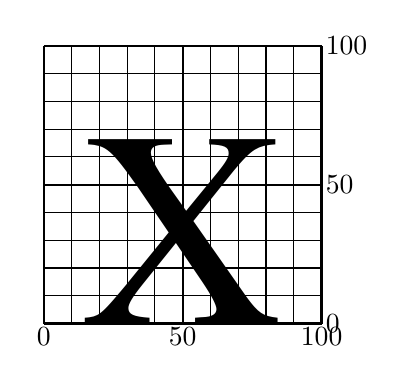
\begin{tikzpicture}[scale=2.54]%
% dpic version 2023.06.01 option -g for TikZ and PGF 1.01
\ifx\dpiclw\undefined\newdimen\dpiclw\fi
\global\def\dpicdraw{\draw[line width=\dpiclw]}
\global\def\dpicstop{;}
\dpiclw=0.8bp
\dpicdraw[line width=0.8bp](0.694444,0.694444)
 --(0.694444,-0.694444)\dpicstop
\draw (0.694444,-0.694444) node[below=-2bp]{0};
\dpicdraw[line width=0.4bp](0.833333,0.694444)
 --(0.833333,-0.694444)\dpicstop
\dpicdraw[line width=0.4bp](0.972222,0.694444)
 --(0.972222,-0.694444)\dpicstop
\dpicdraw[line width=0.4bp](1.111111,0.694444)
 --(1.111111,-0.694444)\dpicstop
\dpicdraw[line width=0.4bp](1.25,0.694444)
 --(1.25,-0.694444)\dpicstop
\dpicdraw[line width=0.8bp](1.388889,0.694444)
 --(1.388889,-0.694444)\dpicstop
\draw (1.388889,-0.694444) node[below=-2bp]{50};
\dpicdraw[line width=0.4bp](1.527778,0.694444)
 --(1.527778,-0.694444)\dpicstop
\dpicdraw[line width=0.4bp](1.666667,0.694444)
 --(1.666667,-0.694444)\dpicstop
\dpicdraw[line width=0.4bp](1.805556,0.694444)
 --(1.805556,-0.694444)\dpicstop
\dpicdraw[line width=0.4bp](1.944444,0.694444)
 --(1.944444,-0.694444)\dpicstop
\dpicdraw[line width=0.8bp](2.083333,0.694444)
 --(2.083333,-0.694444)\dpicstop
\draw (2.083333,-0.694444) node[below=-2bp]{100};
\dpicdraw[line width=0.8bp](0.694444,-0.694444)
 --(2.083333,-0.694444)\dpicstop
\draw (2.083333,-0.694444) node[right=-2bp]{0};
\dpicdraw[line width=0.4bp](0.694444,-0.555556)
 --(2.083333,-0.555556)\dpicstop
\dpicdraw[line width=0.4bp](0.694444,-0.416667)
 --(2.083333,-0.416667)\dpicstop
\dpicdraw[line width=0.4bp](0.694444,-0.277778)
 --(2.083333,-0.277778)\dpicstop
\dpicdraw[line width=0.4bp](0.694444,-0.138889)
 --(2.083333,-0.138889)\dpicstop
\dpicdraw[line width=0.8bp](0.694444,0)
 --(2.083333,0)\dpicstop
\draw (2.083333,0) node[right=-2bp]{50};
\dpicdraw[line width=0.4bp](0.694444,0.138889)
 --(2.083333,0.138889)\dpicstop
\dpicdraw[line width=0.4bp](0.694444,0.277778)
 --(2.083333,0.277778)\dpicstop
\dpicdraw[line width=0.4bp](0.694444,0.416667)
 --(2.083333,0.416667)\dpicstop
\dpicdraw[line width=0.4bp](0.694444,0.555556)
 --(2.083333,0.555556)\dpicstop
\dpicdraw[line width=0.8bp](0.694444,0.694444)
 --(2.083333,0.694444)\dpicstop
\draw (2.083333,0.694444) node[right=-2bp]{100};
\font\testfont=ptmr at 100bp
\draw (1.388889,-0.227083) node(X){\boxdims{Xtest_1}{\testfont X}};
\end{tikzpicture}%
}%
 \end{wrapfigure}%
  One issue is that
  the formatted height of text is generally a fraction of the nominal size.
  For example, the Times letter X at 100\,bp placed on a 100\,bp by
  100\,bp grid is shown at the right.
  The height of the X is
  approximately 66\,bp or 0.66 of the nominal height.
  This ratio depends on the font.
  Consequently, a language issue arises: if the attribute {\tt ht~{\it y}}
  is to be used to set text size,
  should the value of {\it y} be the nominal height (the point size) or
  the formatted height of the text?
% Initial versions of the experimental
% SVG output of \dpic used the
% nominal height but later versions now conform to \LaTeX\ usage by treating
  \Dpic treats {\it y} as the true graphical height in drawing units.
  Thus for example, {\tt "text" ht 10*(scale/72)} produces output
  {\tt 10bp} high.

  To assist with the above and similar issues
  when the {\tt -v} option is invoked, \dpic performs the equivalent
  of
    \ntt{dpPPI = 96}
    \ntt{dptextratio = 0.66}\\
  in the outermost scope of the diagram.  These are ordinary variables
  that can be referenced or changed as usual.
  The variable {\tt dpPPI} is given the inital value 96 which is
  pixels per inch
  on a 20-inch wide computer monitor of 1920 pixels width.
  On such a monitor, dpic output should be close to true size.
  This parameter can be changed using the assignmnent
    \ntt{dpPPI := {\sl value}}\\
  for different screen resolution, and {\tt dptextratio} can
  be similarly changed.
  (For \xfig\ output, the following are defined under the {\tt -x} option:
  {\tt xfdispres = 80; xfigres = 1200}.)


  When \dpic sees the {\tt ht {\it y}} attribute attached to SVG text,
  it sets the nominal text size
  to $y/\tt{dptextratio}$ expressed in points.
  Otherwise, \dpic uses the current value of the environment
  variable {\tt textht}, which has default value $11/72 \times 0.66,$
  to set the default size to 11\,bp.

  The Circuit\_macros configuration file {\tt svg.m4} contains a macro
  {\tt svg\_font} that can simplify font specification, and a macro
  {\tt svgfontratio} that can be used to set {\tt dptextratio} and
  {\tt textht} automatically for common HTML fonts.

  \Dpic sets the width of text
  to the current value of {\tt textwid} by default but,
  as always, it is best not to rely on
  default behaviour. Specify the object (text in this case) completely
  using {\tt wid {\it expression} ht {\it expression}}.
  In the absence of an automatic means of determining it, text width can
  be measured approximately when displayed full-size on a monitor.
  Fortunately on many diagrams, knowing the width is unnecessary or
  is required for only a few key strings.
  In principle, this process might be automated using suitable macros
  and scripting (JavaScript, probably).

\enlargethispage{\baselineskip}
\subsection{Bounding boxes}
  The bounding box of a diagram is not always known exactly or even defined
  exactly, since it can depend on the context in which the diagram is to be
  used.  Within a diagram, different line widths, mitred joints, splines,
  colored output, overpainting, arbitrary text, arbitrary \Postscript or SVG,
  and other complications are allowed; consequently dpic can only provide an
  estimate of the exact bounding box.

  Strategic {\tt move} commands can be used
  to enlarge the bounding box as illustrated at the end of the discussion
  below.

  Dpic uses the constant-width Courier font in pdf files, thus allowing
  the width of strings to be calculated from their height, which is
  specified by {\tt textht} with default $11\,$pt, or by the
  ``{\tt height} {\sl expression}'' attribute.  The string width is calculated
  from the height and character count, but can be set explicitly
  by using {\tt width} {\sl expression} as the rightmost string attribute.

  {\em Psfrag output} is another special case.  If {\tt textht} is set to a
  nonzero value, then its value relative to $11\,$bp is
  given as a scale factor to the psfrag {\tt \tBS{}tex} command.
  An alternative way of changing the diagram text height is to set it in
  the main document; for example,
  {\tt \tLB\tBS{}small \tBS{}includegraphics\tLB{\sl file}.eps\tRB\tRB}.

  {\em Postscript bounding boxes:}
  For a while, the dpic\verb|%%BoundingBox| output line simply gave the nominal
  bounding box determined by line ends and other control points.  The
  use of dpic in server mode has induced a change that correctly
  defines the bounding box for very basic diagrams.  More explicitly,
  consider
\begin{verbatim}
  .PS
  box with .sw at 0,0
  .PE
\end{verbatim}
  which draws a box with southwest corner line centres intersecting at
  \Postscript coordinates 0,0 and northeast intersection at 54,36.
  Dpic {\tt -r} augments this nominal bounding box by half of the last
  {\tt linethick} value (default {\tt linethick} is 0.8 bp)
  in the outermost diagram scope to
  produce the \Postscript bounding-box definitions
\begin{verbatim}
  %%BoundingBox: -1 -1 55 37
  %%HiResBoundingBox: -0.4 -0.4 54.4 36.4
\end{verbatim}
  The\verb|%%BoundingBox| line contains integer values that enclose the
  high-resolution coordinates.

  {\em PDF bounding boxes:}
  PDF includes a MediaBox element which serves approximately the same
  purpose as the postscript BoundingBox, and is calculated the same way.
  By default, dpic puts the lower left corner of PDF output
  at coordinates $(0,0)$.

  {\em Manual bounding box adjustment:}
  It may be necessary to adjust the bounding box manually.  To zero the
  automatic adjustment,
  put {\tt linethick=0} at the end of the outermost scope.
  Then arbitrary margins can be added to the nominal box as shown
  below, where 2, 1, 1, and 0 points are added to the left,
  bottom, right, and top margins respectively:\\
  \ntt{.PS}
  \ntt{Diagram: [}
    \ntt{\quad{\sl drawing commands}}
    \ntt{]}
  \ntt{linethick = 0}
  \ntt{move from Diagram.sw-(2,1)/72*scale to Diagram.ne+(1,0)/72*scale}
  \ntt{.PE}

%===============================================================================

\section{Pic processor differences}\label{Diffs:}
Differences among processors, and between dpic and gpic particularly,
are summarized below.
These differences result from incomplete language definition and
from different implementation contexts.
Normally, the
only changes required to process correct pic or gpic input with dpic are
changes to \tLB$\ldots$\tRB\ instead of {\tt X}$\ldots${\tt X}
syntax as explained below, together with text formatting
if the original code was written for \groff.
Sometimes, differences in default behavior (such as for arcs or object
placement) must be considered.
The remaining items are reasonably small syntactical differences or
relate to the use of \LaTeX\ or the other dpic output formats.

%Gpic is being actively maintained so some of the items below apply only
%to older versions.

\subsection{Command-line options}  They are completely different, of course.
  Type dpic -h to see a list of dpic options.

\subsection{Output formats}
  Gpic {\tt-t} output consists of a sequence of\verb|\special| statements
  contained in the TeX box\verb|\box\graph|.  The\verb|\special| statements
  are
  automatically copied into the {\tt.dvi} file for interpretation by a
  printer driver such as dvips.

  Dpic does not generate tpic specials.
  See the option list in \SR{Usage:} for output formats.

\subsection{``{.}'' and ``\textbackslash''\ lines}
  Gpic passes lines beginning with {\tt.}\ through to the output,
  thereby allowing
  arbitrary Troff macros to be interspersed with pic drawing commands.  Some
  programs that generate pic output automatically insert the Troff line
  \ntt{.ps 11}\\
  on the assumption that the text point size should be 11.  Dpic ignores
  non-continuation lines beginning with {\tt.}\ within pictures.
  Some programs (e.g., pstoedit) add Troff
  comment lines beginning with\verb|.\"| outside the
  {\tt.PS}, {\tt.PE} delimiters.  These
  lines must be dealt with separately.
  Both gpic and dpic pass lines beginning with \tBS\ to the output.

\subsection{{\tt for}-loop and {\tt if} bodies}
  In gpic, a for loop has the form
    \ntt{for {\sl variable} = {\sl expr1} to {\sl expr2}
      {\rm[}by {\rm[}*{\rm]}{\sl expr3}{\rm]} do X {\sl body} X}\\
  where {\tt X} is any character not occurring in {\sl body},
  but \tLB\ {\sl body} \tRB\ is also allowed.
  In dpic only the latter is allowed.
  Similarly, the required form of an if statement for dpic is
    \ntt{if {\sl expr} then \tLB\ {\sl if-true} \tRB\ {\rm[}else
    \tLB\ {\sl if-false} \tRB{\rm]}}

  The test for termination of the multiplicative form of the for loop
  is not identical for dpic and gpic but the effects are identical for
  positive parameters.

  Both gpic and dpic allow the
  loop index variable to be changed within the loop, so infinite
  repetition or control of termination by a test are possible.

\subsection{Closing braces and nul elements}
  In some cases where the contents of {\tt \tLB \tRB} are scanned, a semicolon
  or newline must be inserted prior to the closing brace to ensure that the
  contents of the braces are completed before exit.
  Such a case occurred in the definition of the {\tt case} macro
  on \PR{Branching:}.
  Similarly, a semicolon or newline is required in
  the following {\tt if} test with an {\tt else} clause:
  \ntt{if (sh "test -f fileA.pic")==0 then \tLB $\;$ copy "fileA.pic";
    \tRB \tBS}
  \ntt{else \tLB $\;$ copy "fileB.pic" \tRB}\\
  The semicolon ensures that the {\tt copy} command completes before exiting
  the first pair of braces.

  In the following lines, gpic ignores the {\tt \tLB \tRB} braces
  enclosing the trivial for-loop in the first line and the if-test in the
  second line.  Consequently, the {\tt "x"} labels are misplaced. Dpic
  places the labels correctly.  The cure for gpic is to put a semicolon or
  newline between the rightmost braces.
    \ntt{\tLB for i=1 to 1 do \tLB line right\tRB\tRB; "x"}
    \ntt{move; i=1; \tLB if i==1 \tLB line right\tRB\tRB; "x"}

%\subsection{Nul elements}
  Gpic gives error messages if there is nothing or nothing more than
  newlines or semicolons between ``{\tt \tLB\ \tRB}'' braces or
  ``{\tt [ ]}'' brackets.  These constructs do not occur often in
  hand-generated code (although {\tt []} is sometimes convenient) but
  \Mfour\ or other macros containing conditional expansion can generate
  them unless care is taken to avoid them.
  Dpic allows both items, with {\tt [ ]} generating a block of zero size.

\subsection{End of line}
  The line end is significant in the pic grammar.
  However, dpic ignores line ends following {\tt then}, {\tt \tLB},
  {\tt :}, {\tt else}, or end of line.
  Both the CR (octal 015) and NL (octal 012) characters are treated as
  line ends.

  If the last character of a line is \tBS\ (but not within a string),
  then reading is continued on the next line. Dpic allows this to occur
  within keywords or constants.  Strings can contain multiple lines.

  The {\tt\#} character begins a comment which ends at the end of the line.

  The construction
    \ntt{if {\sl condition} then \tLB\ {\sl if-true} \tRB}
    \ntt{else \tLB\ {\sl if-false} \tRB}\\
  produces an error with all pic interpreters.  To avoid this error, write
    \ntt{if {\sl condition} then \tLB\ {\sl if-true} \tRB\ \tBS}
    \ntt{else \tLB\ {\sl if-false} \tRB}\\

\subsection{Logic}
  Dpic and gpic give slightly different default precedences to the logical
  operators {\tt !}, {\tt \&\&}, {\tt ||}, {\tt ==}, {\tt !=}, {\tt >=},
  {\tt <=}, {\tt <}, and {\tt >}, so judicious use of
  parentheses may sometimes be in order.
  Dpic also requires comparisons and logical operations to be put in
  parentheses in numerical expressions; e.g., 
  \ntt{x = ("{\sl text1}" == "{\sl text2}")}

  The construct {\tt x<A,B>} is intended to have the same meaning as
  {\tt (x between A and B)} but, in some obscure
  circumstances, all pic interpreters have difficulty determining whether
  the {\tt<} character is part of such an expression or is a logical comparison
  operator.  Dpic treats {\tt<}
  as a comparison in the expression following {\tt if} so
  the form {\tt(x between A and B)} should be used in such expressions,
  e.g.
   \ntt{\tt if (0.5 between A and B).y < 2 then }\tLB~$\ldots$ \tRB\\

% In all cases, putting comparisons inside parentheses will
% render them robust to logical agreement and to error messages.

\iffalse
\subsection{{\tt then}}
  Versions of gpic up to 1.19 ignore the {\tt then} keyword, so that
   \ntt{line -> then up 0.5}\\
  draws one line segment and is the same as
   \ntt{line -> up 0.5}\\
  whereas dpic does not ignore {\tt then}, and draws two line segments.
  Newer versions of gpic also draw two segments.
\fi

\subsection{Defaults for {\tt line}, {\tt spline}, {\tt arrow}, {\tt move}}
  Dpic treats the defaults for linear objects consistently with planar
  objects with respect to the {\tt at} modifier.
% Versions of gpic up to 1.19 treated
  Gpic treats
  them differently:

  In dpic, {\tt line at Here} means {\tt line with .center at Here}.\\
  In gpic, {\tt line at Here} means {\tt line with .start at Here}.

  In dpic, the location corresponding to {\tt last line} is
    {\tt last line.c}.\\
  In gpic, the location corresponding to {\tt last line} is
    {\tt last line.start}.

  With dpic,
% In current versions of dpic,
  {\tt last line.wid} returns the arrowhead width of the line or the default
  arrowhead width if the line has not been given an arrowhead;
  similarly for {\tt .ht} and for the other linear objects including {\tt move}
  and, of course, {\tt arrow}.

  The compass corners of multisegmented linear objects are not
  defined in descriptions of the \pic grammar; reasonable positions are
  returned but they should be used with care.

\subsection{Arc defaults}  Gpic and dpic have different algorithms for picking
  a default radius.  The best practice is to specify arcs completely.
  There is also ambiguity in the pic language.  The statement
   \ntt{arc cw rad x from A to B}\\
  does not define a unique arc.
  There are two arcs that satisfy this specification,
  with centres on opposite sides of the line
  joining {\tt A} and {\tt B}.
  Dpic will choose one by attempting to minimize the angle between
  the current direction and the initial tangent of the arc.
  Instead, use
   \ntt{arc cw from A to B with .c at C}

\subsection{Strings} 
% and justified text\label{Strings:}}
Strings are arbitrary character sequences between double quotes.
% with double
%quotes in strings preceded by the backslash character.
Equivalently, a string is produced by the C-like sprintf function
\ntt{sprintf("{\sl format}" {\rm[}, expression,~$\ldots$ {\rm]})}\\
The C snprintf function is used for implementing this; therefore, the
precision of default formats such as {\tt \%g} may vary by machine and compiler.
To produce transportable results, specify the precision completely,
e.g., {\tt \%8.5f}.  As in C, the pair {\tt \%\%}
in the format string prints the percent
character.  Only the {\tt f}, {\tt e}, {\tt g} formatting parameters are
valid, since expressions are stored as floating-point numbers, e.g.
\ntt{line sprintf("\%g\%g0", 2, 0 ) above}\\
is equivalent to
\ntt{line "200" above}

\enlargethispage{\baselineskip}
Similarly,
\ntt{command sprintf("\tBS{}pscircle(\%g,\%g)\tLB\%g\tRB",0,0,0.5)}\\
places a line containing the formatted string without the quotes into
the output.
The numerical {\tt sprintf}
arguments can be arbitrary expressions in place of the constants shown.

  Dpic allows strings to be concatenated by the {\tt+} operator; thus,
  \ntt{"abc" + sprintf(" def\%g",2)}\\
  is equivalent to {\tt"abc def2"}.

  In a macro, a dollar sign followed by an integer in a
  string will expand to the corresponding macro argument if it is
  defined.  Separate the dollar sign from the integer to avoid
  expansion, as in the TeX strings
   {\tt"\tLB\tBS\$\tRB{}1"}, {\tt"\$\tBS\$ 1\$"}, or {\tt"\$\tLB 0\tRB\$"},
  for example.

  Both dpic and gpic treat \tBS\ as an escape character prior to the
  double-quote
  character in a string, so {\tt"\tBS""} is a length-one string containing
  the double quote.  Otherwise, the backslash is an ordinary string
  character.
  For example, the characters\verb|\\"u| in a string are output as\verb|\"u|
  to produce \"u when processed by \LaTeX.
  A string with a backslash as last character
  has to be generated using a macro; for example, if we write
  {\tt define charstr \tLB"\$1"\tRB} then {\tt charstr(abc\tBS)}
  evaluates to a string containing the required final backslash.

  Gpic implements the attribute {\tt aligned} of an object to
  rotate attached strings by sending commands to 
  postprocessor {\tt grops} or {\tt gropdf,}
  which translate troff output to postscript or
  pdf respectively.  The bounding box of the rotated string is unknown.
  Dpic does not define this attribute but allows the user to rotate text
  directly when permitted by the postprocessor.
  For example,
  the Circuit\_macros macro {\tt rs\_box} rotates text for \PSTricks\
  or TikZ-PGF output and calculates the bounding box.
  For SVG output, {\tt svg\_rot()} has a similar function.
  The following simple pic
  macro accomplishes the same goal for \PSTricks\ and \TPGF\ but
  the resulting text bounding box is not calculated.
\begin{verbatim}      
#                           dprtext(degrees,text)
define dprtext {[
  if dpicopt==optPSTricks then {
    sprintf("\rput[c]{%g}(0,0)",$1)+"{$2}"} else {
  if dpicopt==optPGF then {
    sprintf("\pgftext[rotate=%g]",$1)+"{$2}" }}
  ]}
\end{verbatim}      
  Then, for example, {\tt dprtext(45,Hello) at {\sl position}}
  places the text ``Hello'' rotated 45$^{\circ}$ at the specified position.

  A string cannot be assigned to a varable name; the nearest equivalent
  is to define a macro containing the string as the body.

  Both dpic and gpic allow logical comparison of strings.
  Put the comparison in parentheses if it is to be used in an
  expression.

  String height and width are unscaled on final output from dpic since
  these may depend on later formatting by \LaTeX.

  Gpic does not allow newlines in strings; dpic does,
  with an upper limit of 4095 characters.

\subsection{{\tt print} {\sl arg},~$\ldots$}
  Dpic allows only one argument, which may be an expression, position,
  or string.  To print several quantities at once, use
   \ntt{print sprintf($\ldots$)}\\
  to generate a string and, if the string is complicated, remember that
  {\tt {\sl string1} + {\sl string2} +~$\ldots$} evaluates to one string.

\subsection{{\tt command} {\sl arg},~$\ldots$}
  Arbitrary commands are sent to the standard output stream.  Dpic allows only
  one argument, which is a string or {\tt sprintf($\ldots$)}.

\subsection{Operating system commands}
  With dpic, the required form for a shell (operating system) command is
   \ntt{sh "{\sl shell command}"}\\
  or
   \ntt{sh sprintf("{\sl format}",{\sl expression},$\ldots$)}.\\
  The value returned by the operating system can be captured by putting
  the command in parentheses; for example,
   \ntt{if (sh "{\sl shell command}") == 0 then \tLB\ldots\tRB }

\subsection{{\tt copy}}
  \Dpic supports the command
    \ntt{copy "{\sl filename}"}\\
  but does not directly support the \gpic commands
    \ntt{copy {\rm[}{\sl filename}{\rm]}
      thru X {\sl body} X {\rm[} until {\sl word} {\rm]}}
    \ntt{copy {\rm[}{\sl filename}{\rm]}
      thru {\sl macro} {\rm[} until {\sl word} {\rm]}}

  These functions and many more are readily implementable with dpic in any
  Unix-like environment.
%  To customize an operation such as
%    \ntt{copy {\sl filename} thru {\sl macro}}\\
%  modify the following example, as appropriate.
%  This usage is not as
%  simple as a built-in function but allows much more flexibility of data.
%\begin{verbatim}
%  .PS
%  #                               Suppose that file.dat contains rows of data
%  #                               delimited by spaces.
%
%  #                               Macro to process a row of data, e.g.
%  #                               save the first 4 values:
%    define store { n = n+1; x[n] = $1; y[n] = $2; z[n] = $3; w[n] = $4 }
%
%  #                               Use sed to convert the data to a sequence
%  #                               of calls to the store macro:
%    sh "sed -e 's/^ */store(/' -e 's/ *$/)/' -e 's/  */,/g' file.dat >tempfile"
%
%  #                               Initialize the counter and process the data
%    n = 0; copy "tempfile"
%  #                               Delete the temporary file
%    sh "rm tempfile"
%  .PE
%\end{verbatim}
For example, a basic implementation of
{\tt copy {\sl filename} thru {\sl macro}}
is given by the following macro:
\begin{verbatim}
#                               copythru(macro_name,"filename")
#                               Implements copy filename thru macro_name 
#                               for data separated by commas, spaces, or tabs
define copythru { sh "sed -e 's/^[ \t]*/$1(/' -e 's/[ \t]*$/)/' \
  -e 's/[, \t][ \t]*/,/g' $2 > copy_tmp__"
copy "copy_tmp__"
sh "rm -f copy_tmp__" }
\end{verbatim}
The lines of the {\sl filename} file are changed to calls of the {\tt
macro\_name} macro and written into a temporary file, which is then
read by \dpic.  Such usage is not as simple as a built-in function but
allows greater flexibility of data because the {\tt copythru}
macro can be replaced by one customized to suit. For example, the {\tt sh}
command might invoke another program to generate the data.

\subsection{{\tt plot}}
  The {\tt plot} command is deprecated in gpic and not allowed in dpic.

\subsection{{\tt fill}}
  In gpic, a fill value of 0 means white, 1 means black.
  Dpic uses 0 as black and 1 as
  white as do \Postscript and the original ATT pic.

  The pic language specifies fill only for box, ellipse, and circle.
  With dpic, the {\tt shaded} directive fills a path defined by a linear
  object, where allowed by the postprocessor.
  The concept of a path
  containing several arbitrary linear objects does not exist in the pic
  language but can be implemented using postprocessor commands inserted
  into {\tt command {\sl string}} statements.
  Arbitrary paths can also be constructed using a single spline and the
  {\tt continue} statement.

\pagebreak
\subsection{Scaling}
  Dpic implements a {\tt scaled} attribute, so that
  \ntt{box scaled 1.2}\\
  produces a box with dimensions scaled by 1.2, and
  \ntt{[box; line scaled 3; circle] scaled 0.5}\\
  scales all objects within the block by 0.5.  The latter can be used
  when different parts of a diagram require different scaling.
  For example, if file {\tt component.pic} contains a component
  scaled by 25.4, then the following allow it to be used:
  \ntt{[ copy "component.pic" ] scaled 1/25.4}\\
  As always, line thicknesses are not scaled.

\subsection{Arrowheads}
  Pic processors provide a limited variety of built-in arrowhead
  shapes.
  Dpic draws arrowheads according to the environment variable {\tt arrowhead}
  as shown below.
\par
\input arrow.tex
\par
  Any other value of {\tt arrowhead}
  produces the default filled head shown but also
  results in a head shape native to the postprocessor in some cases.
  The default
  value of {\tt arrowhead} is 1 in conformance with other pic processors.
  Postprocessor parameters can be changed using lines of the form
    \ntt{command "{\sl postprocessor commands}"}

% Dpic also allows arrowhead shape to be locally specified by appending
% a parameter after {\tt ->}, {\tt <-}, or {\tt <->}; for example,
%   \ntt{line -> 0 thick 3 wid 0.2 ht 0.3 ... }

  Changing the line thickness does not affect arrowhead size
  parameters, which have to be changed explicitly by either of the
  following methods.  The line thickness is specified in points but the
  arrowhead size parameters are in drawing units:
%\enlargethispage{0.5\baselineskip}\vspace*{-0.5\baselineskip}
\begin{verbatim}
# Method 1 (global change within the current block):
  linethick = 2    # default 0.8 (bp)
  arrowht = 0.18   # default 0.1 (in)
  arrowwid = 0.09  # default 0.05 (in)
  arrowhead = 0    # default 1
  arrow

# Method 2 (put a type 0 arrowhead on the current object):
  arrow -> 0 thick 2 ht 0.18 wid 0.09
\end{verbatim}

  There is a subtle language problem concerning arrowheads.  Let us
  agree that the following examples should all produce an arrow of
  length 1 inch and arrowhead width 1 millimetre:
\begin{verbatim}
  .PS
    arrow right 1 width 1/25.4
  .PE
  .PS
    scale = 25.4
    arrow right 25.4 width 1
  .PE
  .PS 1
    arrow right 1/4 width 1/25.4
  .PE
\end{verbatim}

  The original (ATT) pic fails on the second example, insisting that
  arrowhead dimensions be given in inches.  Gpic fails on the third by
  scaling the arrowhead on final output.  Although it might be argued
  that this is a feature, it causes serious awkwardness when diagrams
  are to be scaled to exact final dimensions using the {\tt.PS} $x$
  construction, since the effective scale factor is unknown until the
  {\tt.PE} line is processed.  Dpic generates the same arrow in all three
  cases, treating arrowhead parameters like line thickness (unscaled)
  parameters on final output.

\subsection{Compass corners and justified text\label{Justified:}}
  Dpic consistently requires a dot before compass corners, so the gpic line
    \ntt{x at center of last box}\\
  should be written for dpic as
    \ntt{x at .center of last box}

Justification is performed by the postprocessor, and combining
justified text with drawing elements requires special consideration.
The lines
  \ntt{S: "Hello" wid 24.7/72 ht 7.6/72 at A ljust}
  \ntt{box wid S.wid ht S.ht at S}\\
produce a box of the correct size but centered at {\tt A} because
the location ({\tt A}) and a justification command are given to the postprocessor.
This behavior could be easily changed but would affect much legacy
code and has been kept for \dpic, which will produce a justified
box using
  \ntt{box wid S.wid ht S.ht with .w at S.w}

\Gpic and \dpic place justified text slightly differently.  In the
previous example, \gpic places the text with its left edge exactly
at {\tt A}, with similar effect for right justification.  \Dpic
uses the environment variable {\tt textoffset}, which is 2.5\,bp by
default, to place the left edge of the text at {\tt A + (textoffset,0)}
with a similar gap for other relative positioning.  Assigning {\tt textoffset}
to 0 sets the gap added by \dpic to zero.

\subsection{{\tt continue}}
  In dpic, the {\tt continue} command appends a linear drawn object to
  the previous drawn object as if {\tt then} had been used in the original
  command, but calculations can be performed to determine size or placement
  of the appended part as in, for example,
   \ntt{line up right}
     \ntt{\quad\sl calculations}
   \ntt{continue down}
     \ntt{\quad\sl more calculations}
   \ntt{continue up left}

  The keyword {\tt continue} can also be used slightly differently. The line
  drawn by
   \ntt{move to (0,0); line right 1 then to (Here,(2,1))}\\
  terminates at {\tt(0,1)} since {\tt Here} is the position {\tt(0,0)},
  whereas the
  following terminates at {\tt(1,1)} since {\tt Here} is {\tt(1,0)}:
   \ntt{move to (0,0); line right 1; continue to (Here,(2,1))}

% Input parsing would be possible if {\tt continue} were to be replaced by
% {\tt then}:
%  \ntt{move to (0,0); line right 1; then to (Here,(2,1))}\\
% The keyword {\tt continue} is not strictly necessary
% but it has been retained for historical compatibility.

\subsection{Subscripted variables and labels}
  Dpic allows subscripted variables and capitalized labels, as described in
  \SR{Subscripts:}.
\iffalse
  as an aid in
  geometric calculations such as fitting splines to a set of points.
  For example, {\tt Pos[{\sl expression}]} is a valid name for a position.
  The rounded integer value of the expression is used.  Up to two subscripts
  are allowed, and 
  {\tt x[{\sl expression},{\sl expression}]} is
  a valid variable name.  There are no array operations, but it is easy
  to write macros for them.
\fi

\subsection{Splines}
  Gpic extends the ATT pic grammar to make {\tt line 0.5} legal and mean
  ``a line of length 0.5 in the current direction.'' All linear objects are
  treated similarly.  Dpic does the same except for splines.  In the
  statement
   \ntt{spline $x$ from A to B then to C}~$\ldots$\\
  the parameter $x$ is a
  tension parameter, normally between 0 and 1, to control the spline
  curvature.  If $x$ is not present as in the normal pic grammar, the
  curve starts with a straight line halfway along the first segment and
  ends with a straight line along the second half of the last segment.
  When $x$ is present however, dpic draws the spline from the start of the
  first segment to the end of the last segment.

\subsection{Arithmetic}
  In an expression, \gpic allows terms of the form {\tt x*-y}, whereas
  \dpic produces an error message. Use {\tt x*(-y)} or the equivalent.

  \Dpic allows the assignment operators {\tt +=}, {\tt -=}, {\tt *=}, 
    {\tt /=}, {\tt \%=}, which do not create a new variable but update
    the value of the variable already defined.
    Thus, the assignment {\tt x += 1} is equivalent to
    {\tt x := x + 1}.

\subsection{Vector arithmetic}
  The dpic grammar permits the following:
  \ntt{X: Y + Z}\\
  where {\tt Y} and {\tt Z} are
  defined positions.  Gpic requires
  \ntt{X: Y + (Z.x,Z.y)}\\
  Dpic also allows
  scalar postmultiplication:
  \ntt{X: Y*2/3}\ (but not {\tt X: 2/3*Y})

\iffalse
\subsection{Positions}
  If {\tt X} is a position, then {\tt (X)} is a valid position for dpic but
  not old versions of gpic, which gave an error for
  \ntt{(a between A and B) + (x,y)}\\
  Dropping the parentheses to avoid the error gives
  \ntt{a between A and B + (x,y)}\\
  which is not the same resulting position. Use dpic or a recent gpic
  if you need this construction.
\fi

\iffalse
\subsection{{\tt int()}}
  Dpic provides
  both the {\tt floor()} and {\tt int()} functions but {\tt int()}
  does not compute the
  same value as pre-1.19 versions of gpic {\tt int()} for non-integer negative
  arguments.
\fi

\subsection{{\tt exec}}
  In dpic the contents of a string can be executed using
   \ntt{exec {\sl string}}\\
  or
   \ntt{exec sprintf({\sl format string}, {\sl args})}\\
  as if the string were the next line of input.  This enables the
  programmed generation of names and labels, for example:
   \ntt{for i=1 to 10 do { exec sprintf("A\%g: x\%g,y\%g",i,2*i,3*i) }}

\subsection{Functions}
A few additional mathematical functions are defined in dpic:
  {\tt abs}, {\tt acos}, {\tt asin}, {\tt expe}, {\tt floor},
  {\tt loge}, {\tt sign}, {\tt tan}, and {\tt pmod}.

%\subsection{PSTricks anomaly}
%  At some time between the years 2000 and 2010,
%  the behaviour of the low-level \PSTricks command
%  {\tt \tBS{}psbezier}
%  was changed to match the existing context-dependent behavior
%  of the {\tt \tBS{}pscurve} command within the\verb|\pscustom| environment%
%\footnote{%
%  The context-dependency of {\tt \tBS{}pscurve} was taken to be a feature
%  rather than a bug.
%  An alternative that preserves command orthogonality would have been
%  to define two curve (and spline) commands for the in-pscustom and out of
%  pscustom contexts.
%% presumably without consideration of independently
%% generated coordinate data.
%% Since curve-defining code then has to be modified
%% depending on where it occurs with respect to {\tt \tBS{}pscustom},
%% the functionality could have been kept while preserving command
%% orthogonality by the use of command options or additional commands.
%  Such are the difficulties of software library maintenance.%
%}.
%  \Dpic does not generate the {\tt \tBS{}pscurve} command,
%  but the new behaviour affects \dpic-defined filled splines.
%  The ``normal'' \PSTricks spline syntax is
%   \ntt{\tBS psbezier(x1,y1)(x2,y2)(x3,y3)(x4,y4)~$\ldots$}\\
%  However, if a correctly defined path containing this spline as its second
%  or later subpath is now enclosed in a\verb|\pscustom| environment, the
%  path coordinates are incorrect;
%% the\verb|\psbezier| command is not the
%% first segment of a path within a\verb|\pscustom| environment then
%  {\tt (x1,y1)} must be omitted since, under these
%  conditions,\verb|\psbezier|
%  takes its first coordinate pair to be the current position.
%  This anomaly would not
%  be a significant problem if it were always known at the time of
%  generating the\verb|\psbezier| coordinates whether the curve will be enclosed
%  within\verb|\pscustom|, but such is not the case.
%
%% Within the pic language in particular, the\verb|\pscustom| command may be
%% introduced via {\tt command} {\sl string} independently of anything else,
%% so \dpic cannot know automatically
%% whether\verb|\pscustom| has been invoked.
%
%  Dpic always generates four (or
%  more) coordinate-pair arguments as in the normal syntax, sometimes
%  resulting in the addition of an extraneous path segment produced
%  within\verb|\pscustom|.
%
%  For some versions of \PSTricks,
%  a workaround for the problem has been to insert a
%  \PSTricks patch in your \LaTeX\ code if you are enclosing splines
%  within\verb|\pscustom| commands.
%  More recent versions of the \PSTricks package have changed
%  again but, starting from the
%  August~27, 2010 {\tt pstricks.tex} distribution file, a parameter
%  {\tt noCurrentPoint} has been introduced,
%  which prevents\verb|\psbezier| (and other commands)
%  from taking the current point as the first coordinate pair.
%  The following line inserted into a latex document avoids an
%  error if the \PSTricks version is August 2010 or later:
%\begin{verbatim}
% \psset{noCurrentPoint}
%\end{verbatim}
%%  As a result, the following file inserted into a latex document seems
%%  to handle both cases in which a workaround is possible: 
%  Older versions of \PSTricks are handled using the following workaround:
%\begin{verbatim}
%command "\makeatletter\@ifundefined{ifPst@noCurrentPoint}%
%{\@ifundefined{MPS@Patch}{\gdef\MPS@Patch{}%
% \typeout{ Dpic -p: patching psbezier in pstricks.tex (some versions) }%
% \def\psbezier@ii{\addto@pscode{%
%  \ifshowpoints true \else false \fi\tx@OpenBezier%
%  \ifshowpoints\tx@BezierShowPoints\fi}\end@OpenObj}}{}}%
%{\@ifundefined{MPS@PatchMsg}{\gdef\MPS@PatchMsg{}%
% \typeout{ Dpic -p: Setting noCurrentPoint to use all coord pairs }}{}%
% \psset{noCurrentPoint}}\makeatother%"
%\end{verbatim}
%
%  This patch need only be executed once per \LaTeX\ run rather than with
%  every diagram.
%
%  If the above fix does not work then, for now,
%  do not insert {\tt spline} commands into paths within the {\tt \tBS pscustom}
%  environment, {\em unless} the spline is the first path segment. It is probably
%  safe to say that this anomaly does not occur very often, but it
%  can cause considerable difficulty when it does; the cure is to update your
%  \PSTricks files.
%
%  Legacy diagrams can often be treated in the following way, if pstricks97.tex
%  is available on your machine as in MiKTeX distributions, for example.
%  Replace the line\verb|\usepackage{pstricks}|
%  with\verb|\usepackage[97]{pstricks}| or\verb|\input{pstricks97.tex}|.
%  However, this method precludes using the newer \PSTricks facilities.

\section{References}
\bibliographystyle{plain}
\renewcommand{\refname}{\vspace*{-\baselineskip}}
\bibliography{./dpic-doc}

%===============================================================================
\clearpage
\section{Appendix A: dpic man page}\label{Appendix A:}
\input dpic_man.tex

%===============================================================================
\clearpage
\section{Appendix B: dpic grammar}\label{Appendix B:}
The tokens recognized by the dpic parser are as shown.  The tokens
in {\tt <} {\tt >} pairs are generated internally.  Equated tokens
({\tt ";" = "<NL>"}) have identical effect.

\begin{verbatim}
    
    terminals:
         "<" "cw" "ccw"
         "(" ")" "*" "+" "-" "/" "%" ";" = "<NL>"
         "^" "!" "&&" "||" 
         "," ":" "[" "]" "{" "}" "." "[]" "`" "'"
         "=" ":=" "+=" "-=" "*=" "/=" "%=" (* the order matters *)
         "&"
         "<float>" "<name>" "<Label>" "<LaTeX>"
         '"' = "<string>"
         "#"
         "$" = "<arg>"
         ".PS" ".PE"
         "ht" = "height" "wid" = "width"
         "rad" = "radius" "diam" = "diameter"
         "thick" = "thickness"
         "scaled"
         "from" "to" "at" "with" "by" "then" "continue"
         "chop" "same"
         "of" "the" "way" "between" "and" "Here"
         "st" = "rd" = "nd" = "th" "last"
         "fill" = "filled"
         ".x" ".y"
         "print" "copy" "reset" "exec" "sh" "command"
         "define" "undef" = "undefine"
         "rand"
         "if" "else" "for" "do" "<endfor>"
         "sprintf"
      "<corner>"
         ".ne" ".se" ".nw" ".sw"
         ".t" = ".top" = "top" = ".north" = ".n"
         ".b" = ".bot" = ".bottom" = "bottom" = ".south" = ".s"
         ".right" = ".r" = ".east" = ".e"
         ".left" = ".l" = ".west" = ".w"
         ".start" = "start"
         ".end" = "end"
         ".center" = ".centre" = ".c"
      "<compare>"
         "==" "!=" ">=" "<=" ">"
      "<param>"
         ".height" = ".ht"
         ".width" = ".wid"
         ".radius" = ".rad"
         ".diameter" = ".diam"
         ".thickness" = ".thick"
         ".length"
      "<func1>"
         "abs" "acos" "asin" "cos" "exp" "expe" "int" "log" "loge"
         "sign" "sin" "sqrt" "tan" "floor"
      "<func2>"
         "atan2" "max" "min" "pmod"
      "<linetype>"
         "solid" "dotted" "dashed" "invis" = "invisible"
      "<colrspec>"
         "color" = "colour" = "colored" = "coloured"
         "outline" = "outlined"
         "shade" = "shaded"
      "<textpos>"
         "centre" = "center" "ljust" "rjust" "above" "below"
      "<arrowhd>"
         "<-" "->" "<->"
      "<directon>"
         "up" "down" "right" "left"
      "<primitiv>"
         "box" "circle" "ellipse" "arc" "line" "arrow" "move" "spline"
      "<envvar>"
        "arcrad" "arrowht" "arrowwid" "boxht" "boxrad" "boxwid"
        "circlerad" "dashwid" "ellipseht" "ellipsewid" "lineht"
        "linewid" "moveht" "movewid" "textht" "textoffset" "textwid"
      = "<lastsc>"          (* marker for last scaled env var *)
        "arrowhead" "fillval" "linethick" "maxpsht" "maxpswid" "scale" 
      = "<lastenv>"         (* marker for last env var *)
\end{verbatim}


The expanded dpic grammar follows:
\begin{verbatim}
input: %empty
     | input picture NL

picture: prestart psline NL elementlist optnl ".PE"

NL: ";"
  | error

prestart: %empty

psline: ".PS"
      | ".PS" term
      | ".PS" term term

elementlist: %empty
           | element
           | elementlist NL element

term: factor
    | term "*" factor
    | term "/" factor
    | term "%" factor

element: namedobj
       | "label" suffix ":" position
       | assignlist
       | "direction: up down right left"
       | "LaTeX"
       | command
       | lbrace elementlist optnl "}"
       | ifpart
       | elsehead elementlist optnl "}"
       | for "}"
       | "command" stringexpr
       | "exec" stringexpr

lbrace: "{"

namedobj: object
        | "label" suffix ":" object

suffix: %empty
      | "[" expression "]"
      | "[" position "]"

position: pair
        | expression "between" position "and" position
        | expression "of" "the" "way" "between" position "and" position
        | expression "<" position "," position "logical operator" shift

assignlist: assignment
          | assignlist "," assignment

command: "print" expression redirect
       | "print" position redirect
       | "print" stringexpr redirect
       | "reset"
       | "reset" resetlist
       | systemcmd
       | "copy" stringexpr
       | "define" "identifier"
       | "define" "label"
       | "undef" "identifier"
       | "undef" "label"

optnl: %empty
     | NL

ifpart: ifhead elementlist optnl "}"

elsehead: ifpart "else" "{"

for: forhead elementlist optnl
   | for forincr elementlist optnl

stringexpr: string
          | stringexpr "+" string

string: "string"
      | sprintf ")"

assignment: "identifier" suffix "=" assignrhs
          | "environment variable" "=" assignrhs

assignrhs: expression
         | assignment

expression: term
          | "+" term
          | "-" term
          | expression "+" term
          | expression "-" term

ifhead: setlogic logexpr "then" "{"

setlogic: "if"

logexpr: logprod
       | logexpr "||" logprod

forhead: "for" assignlist "to" expression do "{"

forincr: "end of for {...} contents"

do: "do"
  | by expression "do"

by: "by"
  | "by" "*"

redirect: %empty
        | "logical operator" stringexpr
        | "logical operator" "logical operator" stringexpr

resetlist: "environment variable"
         | resetlist "," "environment variable"

systemcmd: "sh" stringexpr

sprintf: "sprintf" "(" stringexpr
       | "sprintf" "(" stringexpr "," exprlist

exprlist: expression
        | expression "," exprlist

object: block
      | object "ht" expression
      | object "wid" expression
      | object "rad" expression
      | object "diam" expression
      | object "thick" expression
      | object "scaled" expression
      | object "direction: up down right left" optexp
      | object "line type: dotted etc" optexp
      | object "chop" optexp
      | object "fill" optexp
      | object "arrowhead parameter: <- -> <->" optexp
      | object "then"
      | object "cw"
      | object "ccw"
      | object "same"
      | object stringexpr
      | object "by" position
      | object "from" position
      | object "to" position
      | object "at" position
      | object "text position: ljust rjust above below center"
      | object "color spec: colored outlined shaded" stringexpr
      | objectwith "at" position
      | objectwith "compass corner: .n .ne .center .end etc" "at" position
      | objectwith pair "at" position
      | "continue"

openblock: "["

block: "drawn object: box circle line etc" optexp
     | stringexpr
     | openblock closeblock "]"
     | "[]"

optexp: %empty
      | expression

closeblock: elementlist optnl

objectwith: object "with"
          | objectwith "." "label" suffix
          | objectwith "." nth primobj

pair: expression "," expression
    | location shift

nth: ncount "ordinal: st or rd or nd or th"
   | ncount "ordinal: st or rd or nd or th" "last"
   | "last"

primobj: "drawn object: box circle line etc"
       | "[]"
       | "string"
       | "[" "]"

shift: %empty
     | shift "+" location
     | shift "-" location

location: "(" position ")"
        | "(" position "," position ")"
        | place
        | location "*" factor
        | location "/" factor

place: placename
     | placename "compass corner: .n .ne .center .end etc"
     | "compass corner: .n .ne .center .end etc" placename
     | "compass corner: .n .ne .center .end etc" "of" placename
     | "Here"

factor: primary
      | "!" primary
      | primary "^" factor

placename: "label" suffix
         | nth primobj
         | placename "." "label" suffix
         | placename "." nth primobj

ncount: "number"
      | "`" expression "'"
      | "{" expression "}"

logprod: logval
       | logprod "&&" logval

logval: lcompare
      | stringexpr "<" stringexpr
      | expression "<" expression

lcompare: expression
        | stringexpr
        | lcompare "logical operator" expression
        | lcompare "logical operator" stringexpr

primary: "environment variable"
       | "identifier" suffix
       | "number"
       | "(" logexpr ")"
       | location ".x"
       | location ".y"
       | placename "attribute .ht .wid etc"
       | "rand" "(" ")"
       | "rand" "(" expression ")"
       | "function (1 arg)" "(" expression ")"
       | "function (2 args)" "(" expression "," expression ")"
       | "(" assignlist ")"
       | "(" systemcmd ")"
\end{verbatim}
\end{document}\endinput
